% Documents setup
\documentclass[french,11pt]{book}

% fix for pandoc 1.14
\providecommand{\tightlist}{%
  \setlength{\itemsep}{0pt}\setlength{\parskip}{0pt}}

\usepackage{tabu} % https://tex.stackexchange.com/questions/50332/vertical-spacing-of-a-table-cell

% Location of the csas-style repository: adjust path as needed
\newcommand{\locRepo}{csas-style}

% Use the style file in the csas-style repository (res-doc.sty)
\usepackage{\locRepo/res-doc-french}

% header-includes from R markdown entry


% Headers and footers
\lhead{}
% \lhead{}
\rhead{}
% \rfoot{DRAFT - DO NOT CITE}

%%%% Commands for title page etc %%%%%

% Publication year
\newcommand{\rdYear}{2021}

% Publication month
\newcommand{\rdMonth}{}

% Report number
\newcommand{\rdNumber}{8}

% Region
\newcommand{\rdRegion}{Pacific Region}

% Title
\newcommand{\rdTitle}{Évaluation des stratégies de rétablissement possibles pour le sébaste aux yeux jaunes (\emph{Sebastes ruberrimus}) des eaux intérieures de la Colombie-Britannique}

\newcommand{\rdISBN}{Fs70-5/2021-008F-PDF}
\newcommand{\rdCatNo}{978-0-660-38699-7}

% Author names separated by commas and ', and' for the last author in the format 'M.H. Grinnell' (use \textsuperscript{n} for addresses)
\newcommand{\rdAuth}{Dana R. Haggarty\textsuperscript{1}, Quang C. Huynh\textsuperscript{2}, Robyn E. Forrest\textsuperscript{1}, Sean C. Anderson\textsuperscript{1}, Midoli J. Bresch\textsuperscript{1}, Elise A. Keppel\textsuperscript{1}}

% Author names reversed separated by commas in the format 'Grinnell, M.H.'
\newcommand{\rdAuthRev}{Haggarty, D.R., C.R. Huynh, R.E. Forrest, S.C. Anderson, M.J. Bresch, et E.A. Keppel}

% Author addresses (use \textsuperscript{n})
\newcommand{\rdAuthAddy}{\textsuperscript{1}Station biologique du Pacifique\\
Pêches et Océans Canada, 3190, chemin Hammond Bay\\
Nanaimo (Colombie-Britannique) V9T 6N7, Canada\\
\textsuperscript{2}Institut pour les océans et la pêche\\
LRAE de l'Université de la Colombie- Britannique, 2202, Main Mall\\
Vancouver (Colombie-Britannique) V6T 1Z4, Canada\\}

\newcommand{\citationOtherLanguage}{Haggarty, D.R., Huynh, Q.C., Forrest, R.E., Anderson, S.C., Bresch, M.J., Keppel, E.A. 2021. Evaluation of potential rebuilding strategies for Inside Yelloweye Rockfish (\emph{Sebastes ruberrimus}) in British Columbia. DFO Can. Sci. Advis. Sec. Res. Doc. 2021/008. vi + 141 p.}

% Name of file with abstract and resume (see \abstract and \frenchabstract for requirements)
\newcommand{\rdAbstract}{\abstract{En vertu des politiques et de la législation canadiennes, il faut Eétablir un plan de rétablissement pour les stocks de poissons qui ont été évalués comme étant inférieurs au point de référence limite (PRL) afin de les ramener au-delà du PRL. Les plans de rétablissement doivent être fondés sur des objectifs caractérisés par 1) une cible, 2) un délai souhaité pour atteindre la cible et 3) une probabilité acceptable d'atteindre la cible. Les plans de rétablissement doivent également comprendre des mesures de gestion ou des procédures de gestion, des jalons cibles et être évalués régulièrement. \vspace{1.5mm} \break Le stock de sébaste aux yeux jaunes (\emph{Sebastes ruberrimus}) des eaux intérieures est un stock sur lequel on dispose de données limitées, présent dans la zone de gestion du poisson de fond 4B (détroit de la Reine-Charlotte, détroit de Georgie et détroit de Juan de Fuca) en Colombie-Britannique. Il a été évalué comme étant inférieur au PLR en 2010, ce qui a donné lieu à la publication d'un plan de rétablissement. Il est également inscrit en vertu de la \emph{Loi sur les espèces en péril} comme espèce préoccupante. L'actuelle procédure de gestion pour assurer le rétablissement est un total autorisé des captures (TAC) annuel fixe de 15 tonnes métriques, qui n'a pas été réévalué depuis la dernière évaluation. \vspace{1.5mm} \break Ce projet vise à fournir un avis scientifique à l'appui de la réévaluation du plan de rétablissement du sébaste aux yeux jaunes des eaux intérieures. Nous appliquons un nouveau cadre d'évaluation de la stratégie de gestion (le Cadre des procédures de gestion), récemment élaboré pour le poisson de fond de la Colombie-Britannique, afin d'évaluer le rendement des autres procédures de gestion à données limitées pour ce qui est de l'atteinte des objectifs de rétablissement. Le Cadre des procédures de gestion suit six étapes de pratiques exemplaires pour évaluer la stratégie de gestion~: 1) la définition du contexte décisionnel; 2) l'établissement des objectifs et des paramètres de rendement; 3) la précision des modèles opérationnels pour représenter le système sous-jacent et calculer les paramètres de rendement; 4) la sélection des procédures de gestion possibles; 5) la réalisation de simulations en boucle fermée afin d'évaluer le rendement des procédures de gestion; 6) la présentation des résultats pour faciliter l'évaluation des compromis. \vspace{1.5mm} \break Nous avons appliqué ce cadre pour évaluer le rendement de 34 procédures de gestion à données limitées pour ce qui est de l'atteinte de l'objectif principal, qui est de ramener le stock au-dessus du PRL sur 1,5 génération avec au moins une probabilité de réussite de 95 \% {[}19 fois sur 20{]}. Nous avons également évalué le rendement des procédures de gestion en ce qui concerne deux autres paramètres de conservation, quatre objectifs de prises moyennes et un objectif de variabilité des prises. Pour tenir compte de l'incertitude liée à la dynamique de la population sous-jacente et aux sources de données, nous avons élaboré six scénarios de modèles opérationnels de rechange, qui différaient de par les hypothèses précises du modèle et des données. Ces scénarios de modèles opérationnels ont été divisés en un « ensemble de référence » (quatre modèles opérationnels) et un « ensemble de robustesse » (deux modèles opérationnels). Nous avons conditionné tous les modèles opérationnels aux données sur les prises observées, aux indices de l'abondance et aux données accessibles sur la composition selon l'âge. Nous avons utilisé la simulation en boucle fermée pour évaluer le rendement des procédures de gestion et nous avons éliminé celles qui ne satisfaisaient pas à un ensemble de critères de base, ce qui a laissé cinq procédures de gestion possibles~: des procédures de gestion à prises constantes annuelles de 10 ou 15 tonnes et trois procédures de gestion qui ajustent le TAC en fonction de la pente relative de l'indice de l'abondance dans le relevé à la palangre sur fond dur dans les eaux intérieures. \vspace{1.5mm} \break Les cinq procédures de gestion finales atteignaient l'objectif principal avec une probabilité supérieure à 0,98 (49 fois sur 50), dans les scénarios des quatre modèles opérationnels de l'ensemble de référence, surtout qu'aucun des modèles opérationnels de l'ensemble de référence n'a estimé que le stock serait inférieur au PRL en 2020. Dans les scénarios des deux modèles opérationnels de l'ensemble de robustesse, le scénario qui simulait une plus grande variabilité dans le futur relevé à la palangre sur fond dur a donné des résultats semblables à ceux des scénarios de l'ensemble de référence. Cependant, dans le scénario qui supposait un taux de mortalité naturelle plus faible pour le stock (« M faible »), toutes les procédures de gestion avaient des probabilités plus basses d'atteindre l'objectif principal, la probabilité la plus faible étant atteinte par la procédure de gestion actuelle (prises constantes de 15 tonnes). \vspace{1.5mm} \break Nous présentons un certain nombre de visualisations pour illustrer les compromis entre les objectifs de conservation et de prises pour les différentes procédures de gestion dans d'autres scénarios de modèles opérationnels. Ces visualisations présentent les compromis sous forme de tableaux et de graphiques, destinés à faciliter le processus de sélection de la procédure de gestion finale. Étant donné que toutes les procédures de gestion ont atteint l'objectif principal dans les scénarios de l'ensemble de référence, il n'y avait pas de compromis important entre les objectifs de conservation et les objectifs de prises. Parmi les deux scénarios de l'ensemble de robustesse, les compromis étaient les plus évidents dans le scénario de M faible, où la probabilité d'atteindre l'objectif principal diminuait à mesure que la probabilité de prises moyennes à court terme de 10 tonnes augmentait. \vspace{1.5mm} \break Nous discutons des incertitudes majeures, y compris l'incertitude entourant la mortalité naturelle, la sélectivité et les prises historiques, en notant que nous avons tenté d'en tenir compte en évaluant le rendement des procédures de gestion dans plusieurs modèles opérationnels. Nous soulignons les problèmes concernant les estimations de l'état actuel du stock de sébaste aux yeux jaunes des eaux intérieures et le rôle des points de référence dans le Cadre des procédures de gestion. Nous formulons des recommandations sur la fréquence des évaluations et suggérons des déclencheurs pour la réévaluation. Nous évaluons également le rendement des procédures de gestion en ce qui concerne le respect de deux autres critères d'évaluation pour le Comité sur la situation des espèces en péril au Canada.}}

%%%% End of title page commands %%%%%

% \pdfcompresslevel=5 % faster PNGs

\setcounter{section}{0}

\bibliographystyle{csas-style/res-doc}

\usepackage{amsmath}
\usepackage{bm}

% commands and environments needed by pandoc snippets
% extracted from the output of `pandoc -s`
%% Make R markdown code chunks work
\usepackage{array}
\usepackage{amssymb,amsmath}
\usepackage{color}
\usepackage{fancyvrb}
% From default template:
\newcommand{\VerbBar}{|}
\newcommand{\VERB}{\Verb[commandchars=\\\{\}]}
\DefineVerbatimEnvironment{Highlighting}{Verbatim}{commandchars=\\\{\}}
% Add ',fontsize=\small' for more characters per line
\usepackage{framed}
\definecolor{shadecolor}{RGB}{248,248,248}
\newenvironment{Shaded}{\begin{snugshade}}{\end{snugshade}}
\newcommand{\AlertTok}[1]{\textcolor[rgb]{0.94,0.16,0.16}{#1}}
\newcommand{\AnnotationTok}[1]{\textcolor[rgb]{0.56,0.35,0.01}{\textbf{\textit{#1}}}}
\newcommand{\AttributeTok}[1]{\textcolor[rgb]{0.77,0.63,0.00}{#1}}
\newcommand{\BaseNTok}[1]{\textcolor[rgb]{0.00,0.00,0.81}{#1}}
\newcommand{\BuiltInTok}[1]{#1}
\newcommand{\CharTok}[1]{\textcolor[rgb]{0.31,0.60,0.02}{#1}}
\newcommand{\CommentTok}[1]{\textcolor[rgb]{0.56,0.35,0.01}{\textit{#1}}}
\newcommand{\CommentVarTok}[1]{\textcolor[rgb]{0.56,0.35,0.01}{\textbf{\textit{#1}}}}
\newcommand{\ConstantTok}[1]{\textcolor[rgb]{0.00,0.00,0.00}{#1}}
\newcommand{\ControlFlowTok}[1]{\textcolor[rgb]{0.13,0.29,0.53}{\textbf{#1}}}
\newcommand{\DataTypeTok}[1]{\textcolor[rgb]{0.13,0.29,0.53}{#1}}
\newcommand{\DecValTok}[1]{\textcolor[rgb]{0.00,0.00,0.81}{#1}}
\newcommand{\DocumentationTok}[1]{\textcolor[rgb]{0.56,0.35,0.01}{\textbf{\textit{#1}}}}
\newcommand{\ErrorTok}[1]{\textcolor[rgb]{0.64,0.00,0.00}{\textbf{#1}}}
\newcommand{\ExtensionTok}[1]{#1}
\newcommand{\FloatTok}[1]{\textcolor[rgb]{0.00,0.00,0.81}{#1}}
\newcommand{\FunctionTok}[1]{\textcolor[rgb]{0.00,0.00,0.00}{#1}}
\newcommand{\ImportTok}[1]{#1}
\newcommand{\InformationTok}[1]{\textcolor[rgb]{0.56,0.35,0.01}{\textbf{\textit{#1}}}}
\newcommand{\KeywordTok}[1]{\textcolor[rgb]{0.13,0.29,0.53}{\textbf{#1}}}
\newcommand{\NormalTok}[1]{#1}
\newcommand{\OperatorTok}[1]{\textcolor[rgb]{0.81,0.36,0.00}{\textbf{#1}}}
\newcommand{\OtherTok}[1]{\textcolor[rgb]{0.56,0.35,0.01}{#1}}
\newcommand{\PreprocessorTok}[1]{\textcolor[rgb]{0.56,0.35,0.01}{\textit{#1}}}
\newcommand{\RegionMarkerTok}[1]{#1}
\newcommand{\SpecialCharTok}[1]{\textcolor[rgb]{0.00,0.00,0.00}{#1}}
\newcommand{\SpecialStringTok}[1]{\textcolor[rgb]{0.31,0.60,0.02}{#1}}
\newcommand{\StringTok}[1]{\textcolor[rgb]{0.31,0.60,0.02}{#1}}
\newcommand{\VariableTok}[1]{\textcolor[rgb]{0.00,0.00,0.00}{#1}}
\newcommand{\VerbatimStringTok}[1]{\textcolor[rgb]{0.31,0.60,0.02}{#1}}
\newcommand{\WarningTok}[1]{\textcolor[rgb]{0.56,0.35,0.01}{\textbf{\textit{#1}}}}

\newcommand{\lt}{\ensuremath <}
\newcommand{\gt}{\ensuremath >}

%Defines cslreferences environment
%Required by pandoc 2.8
%Copied from https://github.com/rstudio/rmarkdown/issues/1649

\DeclareGraphicsExtensions{.png,.pdf}
\begin{document}
\renewcommand{\tablename}{Tableau}
\frontmatter

\clearpage

\hypertarget{sec:introduction}{%
\section{INTRODUCTION}\label{sec:introduction}}

Ce projet vise à fournir un avis scientifique à l'appui de la révision du plan de rétablissement du stock de sébaste aux yeux jaunes (\emph{Sebastes ruberrimus}) des eaux intérieures (DFO \protect\hyperlink{ref-ifmp2018}{2018}), conformément aux directives stratégiques nationales (DFO \protect\hyperlink{ref-dfo2009}{2009}, \protect\hyperlink{ref-dfo2013}{2013}). Il applique un cadre de simulation en boucle fermée (Anderson et al. \protect\hyperlink{ref-anderson2020gfmp}{2020}\protect\hyperlink{ref-anderson2020gfmp}{b}) pour évaluer le rendement des procédures de gestion de rechange en ce qui concerne les objectifs de rétablissement du stock de sébaste aux yeux jaunes des eaux intérieures.

\hypertarget{sec:introduction-motivation}{%
\subsection{MOTIVATION~: OBLIGATIONS STRATÉGIQUES ET LÉGISLATIVES}\label{sec:introduction-motivation}}

Le Cadre pour la pêche durable du Canada jette les bases de l'approche de précaution en matière de gestion des pêches au Canada (DFO \protect\hyperlink{ref-dfo2006}{2006}, \protect\hyperlink{ref-dfo2009}{2009}). Le Cadre de l'approche de précaution (DFO \protect\hyperlink{ref-dfo2009}{2009}) repose sur la définition des points de référence biologiques qui définissent les cibles de la biomasse ainsi que les seuils de biomasse faible à éviter avec une probabilité élevée. L'approche exige que la mortalité par pêche soit ajustée par rapport à deux niveaux de l'état des stocks~: un point de référence supérieur du stock (RSS) et un point de référence limite (PRL) (figure~\ref{fig:pa-illustration}). Le PRL et le RSS délimitent trois zones d'état des stocks (« critique », « de prudence » et « saine »). Il faut établir un plan de rétablissement pour les stocks de poissons canadiens qui ont été évalués comme étant inférieurs au PRL, c.-à-d.~dans la zone critique (DFO \protect\hyperlink{ref-dfo2009}{2009}), afin de les ramener au-dessus du PRL (DFO \protect\hyperlink{ref-dfo2013}{2013}).


\begin{figure}[htb]

{\centering \pdftooltip{\includegraphics[width=3.8in]{C:/GitHub/yelloweye-inside/figs-french/pa-framework}}{Figure \ref{fig:pa-illustration}} 

}

\caption{Illustration du Cadre de l'approche de précaution du MPO. D'après DFO (\protect\hyperlink{ref-dfo2009}{2009}).}\label{fig:pa-illustration}
\end{figure}
En juin 2019, d'importantes modifications apportées à la \emph{Loi sur les pêches} du Canada ont légiféré de nombreux éléments clés du Cadre pour la pêche durable, qui sont enchâssés dans les dispositions sur les stocks de poissons (\href{https://laws-lois.justice.gc.ca/fra/lois/f-14/page-3.html\#h-1175547}{article 6 de la \emph{Loi sur les pêches}}. Les dispositions relatives aux stocks de poissons exigent que les principaux stocks soient gérés à des niveaux durables, en particulier à des niveaux de biomasse supérieurs au PRL. De plus, le paragraphe 6.2(1) stipule que si un grand stock de poissons a diminué en deçà de son PRL, un plan de rétablissement doit être établi pour reconstituer le stock au-dessus du PRL. Les grands stocks de poissons seront désignés en vertu d'un règlement, le premier lot de stocks devant l'être à l'automne 2020.

En vertu des directives sur l'élaboration de plans de rétablissement au Canada (DFO \protect\hyperlink{ref-dfo2013}{2013}), les plans de rétablissement doivent être fondés sur des objectifs caractérisés par~:
\begin{enumerate}
\def\labelenumi{\arabic{enumi}.}

\item
  une cible;
\item
  un délai souhaité pour atteindre la cible;
\item
  une probabilité acceptable convenue d'atteindre la cible.
\end{enumerate}
Les plans de rétablissement doivent également comprendre des mesures de gestion planifiées (les procédures de gestion), des jalons cibles et leur rendement doit faire l'objet d'examens réguliers (tous les trois ans), en plus de la surveillance et de l'évaluation annuelles. Les directives actuelles indiquent que le délai de rétablissement doit être de 1,5 à 2 fois la durée de génération de l'espèce (DFO \protect\hyperlink{ref-dfo2013}{2013}), la durée de génération étant le nombre moyen d'années entre la naissance d'un individu et la naissance de sa progéniture.

\hypertarget{sec:introduction-background}{%
\subsection{CONTEXTE}\label{sec:introduction-background}}

Le sébaste aux yeux jaunes des eaux intérieures est présent dans la zone de gestion 4B du poisson de fond en Colombie-Britannique (Figure~\ref{fig:map-4B}). Il devrait être désigné comme grand stock de poissons à l'automne 2020, date à laquelle sa gestion sera légiférée en vertu des dispositions sur les stocks de poissons. Le stock a été évalué comme étant inférieur au PLR en 2010 (Yamanaka et al. \protect\hyperlink{ref-yamanaka2011}{2011}; DFO \protect\hyperlink{ref-dfo2012}{2012}\protect\hyperlink{ref-dfo2012}{a}). De ce fait, un plan de rétablissement a été élaboré et publié à l'annexe 9 du Plan de gestion intégrée des pêches de la région du Pacifique pour le poisson de fond (DFO \protect\hyperlink{ref-ifmp2018}{2018}). Le stock de sébaste aux yeux jaunes des eaux intérieures est également inscrit en vertu de la \emph{Loi sur les espèces en péril} (LEP) comme espèce préoccupante (COSEWIC \protect\hyperlink{ref-cosewic2008}{2008}\protect\hyperlink{ref-cosewic2008}{a}) et il est prévu que le Comité sur la situation des espèces en péril au Canada (COSEPAC) le réévaluera en 2020. Les résultats de ce projet pourraient guider la réévaluation du COSEPAC et, éventuellement, une évaluation du potentiel de rétablissement en vertu de la LEP, s'il y a lieu (voir l'annexe~\ref{app:cosewic}).


\begin{figure}[htb]

{\centering \pdftooltip{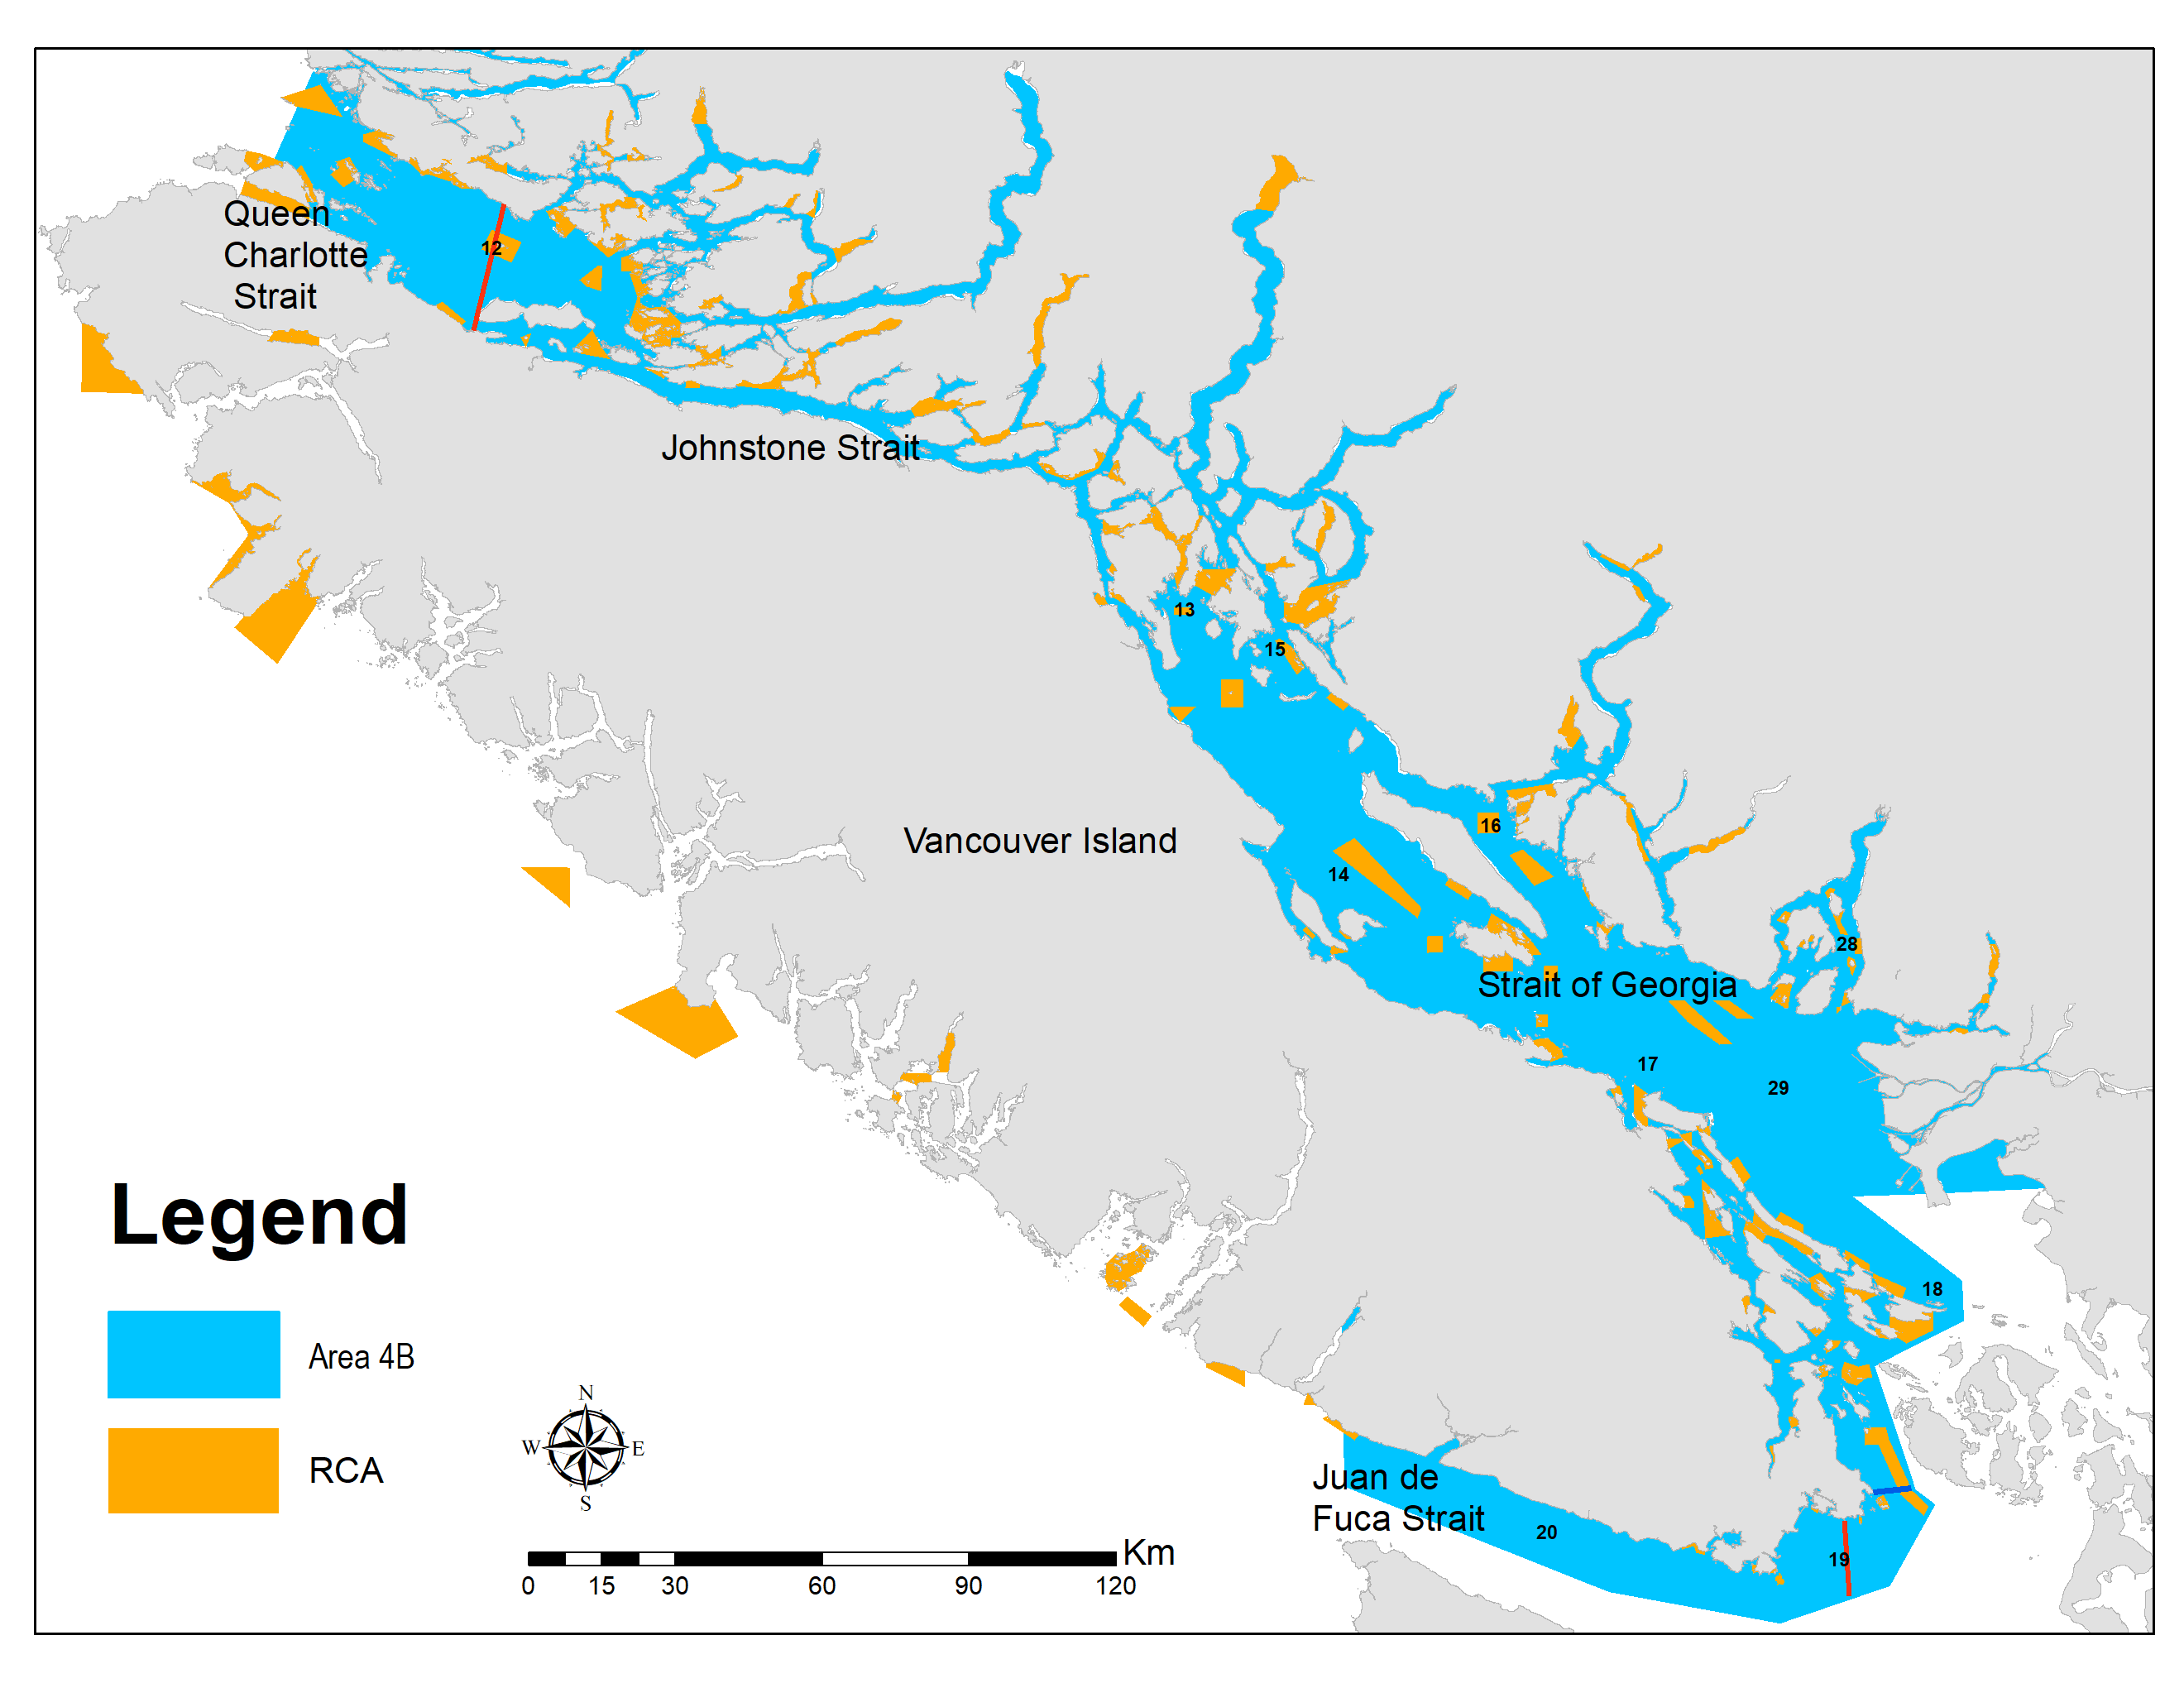
\includegraphics[width=5in]{C:/GitHub/yelloweye-inside/figs-french/InsideYE_Map_new}}{Figure \ref{fig:map-4B}} 

}

\caption{Carte de la zone de gestion 4B du poisson de fond montrant les aires de conservation du sébaste (ACS) et les limites séparant l'unité désignable (UD) du sébaste aux yeux jaunes des eaux intérieures de l'UD du sébaste aux yeux jaunes des eaux extérieures. Les lignes rouges indiquent une proposition d'ajustement de l'aire de répartition de l'UD des eaux intérieures, fondée sur des preuves génétiques récentes (Siegle \protect\hyperlink{ref-siegle2011}{2011}; Siegle et al. \protect\hyperlink{ref-siegle2013}{2013}; Andrews et al. \protect\hyperlink{ref-andrews2018}{2018}).}\label{fig:map-4B}
\end{figure}
L'objectif du plan de rétablissement actuel est de « reconstituer le stock au-dessus du PRL sur 80 ans avec une probabilité de réussite de 56 \% ». Le jalon cible est de « dégager des tendances positives au cours de chaque période de 10 ans ». La procédure de gestion actuelle du sébaste aux yeux jaunes des eaux intérieures vise à maintenir les prises annuelles totales (commerciales, récréatives, alimentaires, sociales et rituelles des Premières Nations et de relevé) à moins de 15 tonnes (voir l'annexe 9 du document DFO (\protect\hyperlink{ref-ifmp2018}{2018}) pour plus de renseignements).

D'après les directives, les plans de rétablissement au Canada doivent présenter une forte probabilité de rétablissement des stocks de poissons hors de la zone critique dans le délai prescrit (DFO \protect\hyperlink{ref-dfo2013}{2013}). Ce projet vise notamment à répondre à une préoccupation exprimée par les gestionnaires des pêches, à savoir que la probabilité de réussite de 56 \% énoncée dans le plan de rétablissement actuel (DFO \protect\hyperlink{ref-ifmp2018}{2018}) ne correspond pas à la définition d'une probabilité élevée.

Le document d'orientation indique également certaines mesures de gestion recommandées, comme le maintien des prélèvements par toutes les sources au niveau le plus bas possible, l'élaboration d'une règle de contrôle des prises et l'application de l'évaluation de la stratégie de gestion pour évaluer, par simulation, le rendement d'autres mesures de gestion pour atteindre les objectifs de rétablissement du stock (DFO \protect\hyperlink{ref-dfo2013}{2013}). Le plan de rétablissement actuel met en œuvre un total autorisé des captures annuel fixe de 15 tonnes (DFO \protect\hyperlink{ref-ifmp2018}{2018}), qui n'a pas été mis à l'essai par simulation.

Le sébaste aux yeux jaunes est une espèce qui vit longtemps (jusqu'à 121 ans en Colombie-Britannique, Keppel et Olsen \protect\hyperlink{ref-keppel2019}{2019}), dans des habitats démersaux rocheux répartis de manière irrégulière et discontinue sur la côte intérieure de la Colombie-Britannique (Yamanaka et al. \protect\hyperlink{ref-yamanaka2011}{2011}). Ces caractéristiques du cycle biologique rendent l'espèce vulnérable à la surexploitation par la pêche. Le stock des eaux intérieures est considéré comme étant à données limitées, car peu de données sont accessibles sur la composition selon l'âge, on manque de données biologiques sur les pêches commerciales, récréatives et des Premières Nations, et une incertitude entoure l'ampleur des prises historiques.

\hypertarget{sec:introduction-mse}{%
\subsection{ÉVALUATION DE LA STRATÉGIE DE GESTION}\label{sec:introduction-mse}}

À l'échelle mondiale, la fourniture d'avis scientifiques pour la gestion des pêches a évolué vers des approches axées sur l'évaluation de la stratégie de gestion (ou axées sur la gestion) (p.~ex., Butterworth et Punt \protect\hyperlink{ref-butterworth1999}{1999}; Rademeyer et al. \protect\hyperlink{ref-rademeyer2007}{2007}; Berkson et Thorson \protect\hyperlink{ref-berkson2015}{2015}; Geromont et Butterworth \protect\hyperlink{ref-geromont2015}{2015}; Carruthers et al. \protect\hyperlink{ref-carruthers2016}{2016}; Punt et al. \protect\hyperlink{ref-punt2016}{2016}). L'évaluation de la stratégie de gestion se concentre sur la détermination des procédures de gestion qui donnent les meilleurs résultats en ce qui concerne l'atteinte des objectifs convenus en matière de politique et de pêche, lorsqu'ils sont mis en œuvre dans un environnement de simulation en « boucle fermée » (figure~\ref{fig:mse-chart-basic}). Dans les pêches à production contrôlée, comme la pêche du poisson de fond en Colombie-Britannique, où les quotas sont gérés, les procédures de gestion décrivent les mesures de gestion pour l'établissement des limites des prises. Les données exigées dans les procédures de gestion peuvent varier considérablement, allant d'approches très riches en données, y compris les évaluations statistiques des prises selon l'âge avec des règles de contrôle des prises, à des règles de données simples (approches « limitées en données »), qui ne reposent que sur les données sur les prises et un indice de l'abondance (p.~ex., Geromont et Butterworth \protect\hyperlink{ref-geromont2015}{2015}; Carruthers et al. \protect\hyperlink{ref-carruthers2016}{2016}).

La simulation en boucle fermée diffère des approches d'évaluation classique des stocks parce qu'elle simule la rétroaction entre la mise en œuvre des procédures de gestion et le système sous-jacent (le stock de poisson et son environnement), décrite par un ou plusieurs modèles opérationnels. L'approche de la simulation en boucle fermée tient compte de l'effet des procédures de gestion sur le système, ainsi que des données futures recueillies dans le système et de leur utilisation chez les procédures de gestion (Punt et al. \protect\hyperlink{ref-punt2016}{2016}; Carruthers et Hordyk \protect\hyperlink{ref-carruthers2018}{2018}\protect\hyperlink{ref-carruthers2018}{a}; Anderson et al. \protect\hyperlink{ref-anderson2020gfmp}{2020}\protect\hyperlink{ref-anderson2020gfmp}{b}).


\begin{figure}[htb]

{\centering \pdftooltip{\includegraphics[width=6.3in]{C:/GitHub/yelloweye-inside/figs-french/mse-chart-simple2}}{Figure \ref{fig:mse-chart-basic}} 

}

\caption{Illustration du processus de simulation en boucle fermée des pêches d'après Anderson et al. (\protect\hyperlink{ref-anderson2020gfmp}{2020}\protect\hyperlink{ref-anderson2020gfmp}{b}), selon Punt et al. (\protect\hyperlink{ref-punt2016}{2016}). La procédure de gestion peut être fondée sur une règle de données simple (p.~ex., réduire les prises autorisées de x \% si l'indice du relevé diminue de y \%) ou peut être un modèle d'estimation combiné à une règle de contrôle des prises.}\label{fig:mse-chart-basic}
\end{figure}
\hypertarget{sec:introduction-approach}{%
\subsection{APPROCHE}\label{sec:introduction-approach}}

En raison des données limitées sur le stock de sébaste aux yeux jaunes des eaux intérieures, il est difficile d'évaluer le rendement prévu des mesures de gestion nécessaires pour rendre le stock conforme aux dispositions sur les stocks de poissons, c.-à-d.~pour le faire sortir de la zone critique dans le délai convenu et avec la probabilité convenue. La simulation-mise à l'essai en boucle fermée des procédures de gestion à données limitées permet d'évaluer le rendement relatif des procédures de gestion dans un éventail d'incertitudes entourant, par exemple, la biologie sous-jacente des poissons, l'erreur d'observation, l'erreur d'estimation et l'erreur de mise en œuvre (p.~ex., Kell et al. \protect\hyperlink{ref-kell2006}{2006}; Carruthers et al. \protect\hyperlink{ref-carruthers2016}{2016}).

Depuis 2017, une entente de partenariat entre l'Université de la Colombie-Britannique et le MPO (DFO \protect\hyperlink{ref-dfo_dlmtool_2017}{2017}) a facilité l'élaboration de deux progiciels à accès libre pour l'évaluation de la stratégie de gestion, mis en œuvre dans l'environnement de programmation statistique R (R Core Team \protect\hyperlink{ref-r2019}{2019})~: l'outil pour les méthodes à données limitées (DLMtool) (Carruthers et Hordyk \protect\hyperlink{ref-carruthers2018}{2018}\protect\hyperlink{ref-carruthers2018}{a}, \protect\hyperlink{ref-carruthers_hordyk_2018}{2018}\protect\hyperlink{ref-carruthers_hordyk_2018}{b}) et l'outil pour l'évaluation de la stratégie de gestion (MSEtool) (Huynh et al. \protect\hyperlink{ref-huynh_msetool_2019}{2019}). Après plusieurs années de développement, ces progiciels sont parmi les logiciels les plus rapides, les plus souples et les plus extensibles pour évaluer les stratégies de gestion des pêches. Ils peuvent être appliqués à des stocks pauvres ou riches en données, permettant d'évaluer rapidement plusieurs procédures de gestion en fonction d'objectifs de conservation et de pêche personnalisables, et d'évaluer les principaux compromis.

\hypertarget{sec:introduction-mp-framework}{%
\subsubsection{Cadre des procédures de gestion du poisson de fond en Colombie-Britannique}\label{sec:introduction-mp-framework}}

Le Cadre des procédures de gestion pour le poisson de fond en Colombie-Britannique (Anderson et al. \protect\hyperlink{ref-anderson2020gfmp}{2020}\protect\hyperlink{ref-anderson2020gfmp}{b}) a été élaboré parallèlement au présent document pour évaluer le rendement d'un large éventail de procédures de gestion pour les espèces de poisson de fond à données limitées. Le Cadre des procédures de gestion fait largement appel aux fonctions de DLMtool et de MSEtool, avec l'appui d'un progiciel R gfdlm (Anderson et al. \protect\hyperlink{ref-gfdlm}{2020}\protect\hyperlink{ref-gfdlm}{d}) rédigé par les auteurs de Anderson et al. (\protect\hyperlink{ref-anderson2020gfmp}{2020}\protect\hyperlink{ref-anderson2020gfmp}{b}), qui contient un ensemble d'outils de soutien logiciel et des visualisations personnalisées.

Nous suivons le Cadre des procédures de gestion pour sélectionner les procédures de gestion afin d'établir des limites des prises pour les stocks de poissons de fond à données limitées (Anderson et al. \protect\hyperlink{ref-anderson2020gfmp}{2020}\protect\hyperlink{ref-anderson2020gfmp}{b}). Notre évaluation du plan de rétablissement du sébaste aux yeux jaunes des eaux intérieures constitue la première application du Cadre des procédures de gestion pour produire un avis scientifique à l'appui des décisions sur les prises. Le cadre suit six étapes de pratiques exemplaires décrites ci-après et plus en détail dans Anderson et al. (\protect\hyperlink{ref-anderson2020gfmp}{2020}\protect\hyperlink{ref-anderson2020gfmp}{b}).

Les étapes des pratiques exemplaires sont fondées sur un examen effectué par Punt et al. (\protect\hyperlink{ref-punt2016}{2016}), qui a cerné cinq étapes clés du processus d'évaluation de la stratégie de gestion (étapes 2 à 6 ci-après). Une première étape supplémentaire du Cadre des procédures de gestion, qui définit le contexte décisionnel, a été définie par Gregory et al. (\protect\hyperlink{ref-gregory2012}{2012}) et Cox et Benson (\protect\hyperlink{ref-cox2016}{2016}). En grande partie, le logiciel DLMtool a été conçu pour permettre aux praticiens de suivre ces étapes (figure~\ref{fig:mse-chart}; Carruthers et Hordyk \protect\hyperlink{ref-carruthers2018}{2018}\protect\hyperlink{ref-carruthers2018}{a}).


\begin{figure}[htb]

{\centering \pdftooltip{\includegraphics[width=\textwidth]{C:/GitHub/yelloweye-inside/figs-french/mse-chart}}{Figure \ref{fig:mse-chart}} 

}

\caption{Les étapes du processus d'évaluation de la stratégie de gestion selon Punt et al. (\protect\hyperlink{ref-punt2016}{2016}), tel que mis en œuvre dans DLMtool. Copié de Anderson et al. (\protect\hyperlink{ref-anderson2020gfmp}{2020}\protect\hyperlink{ref-anderson2020gfmp}{b}) et adapté de Carruthers et Hordyk (\protect\hyperlink{ref-carruthers2018}{2018}\protect\hyperlink{ref-carruthers2018}{a}). Cette figure complète la figure~\ref{fig:mse-chart-basic}.}\label{fig:mse-chart}
\end{figure}
Les six étapes sont les suivantes~:

Étape 1~: Définition du contexte décisionnel.

Étape 2~: Choix des objectifs et des paramètres de rendement.

Étape 3~: Choix des incertitudes/spécification des modèles opérationnels.

Étape 4~: Détermination des procédures de gestion possibles.

Étape 5~: Simulation de l'application des procédures de gestion.

Étape 6~: Présentation des résultats et choix de la procédure de gestion.

Après la sélection et la mise en œuvre de la procédure de gestion pour l'établissement de la limite des prises (figure~\ref{fig:mse-chart}; par exemple, application de l'algorithme de la procédure de gestion sélectionnée à l'indice du relevé observé), la dernière étape nécessaire consiste à surveiller et à évaluer périodiquement le rendement de la procédure de gestion (DFO \protect\hyperlink{ref-dfo2013}{2013}; Dowling et al. \protect\hyperlink{ref-dowling2015a}{2015}; Carruthers et Hordyk \protect\hyperlink{ref-carruthers2018}{2018}\protect\hyperlink{ref-carruthers2018}{a}). Cela peut se faire par des moyens informels, comme à l'aide de la rétroaction des pêcheurs et des données des relevés (p.~ex., Cox et Kronlund \protect\hyperlink{ref-cox2008a}{2008}), ou au moyen de mesures statistiques plus formelles, où l'on compare les données observées aux prévisions des modèles opérationnels pour vérifier si le système fonctionne comme prévu (Butterworth \protect\hyperlink{ref-butterworth2008}{2008}; Carruthers et Hordyk \protect\hyperlink{ref-carruthers_hordyk_2018}{2018}\protect\hyperlink{ref-carruthers_hordyk_2018}{b}; discussion dans Anderson et al. \protect\hyperlink{ref-anderson2020gfmp}{2020}\protect\hyperlink{ref-anderson2020gfmp}{b}).

Dans les sections suivantes, nous décrivons notre approche pour l'élaboration d'un éventuel plan de rétablissement du sébaste aux yeux jaunes des eaux intérieures, en suivant les six étapes des pratiques exemplaires.

\hypertarget{sec:decision-context}{%
\section{DÉFINIR LE CONTEXTE DÉCISIONNEL}\label{sec:decision-context}}

Les principales questions qui guident la définition du contexte décisionnel de l'évaluation de la stratégie de gestion sont les suivantes~:
\begin{itemize}
\item
  Quelle est la décision exacte à prendre?
\item
  Quel est le délai pour prendre la décision?
\item
  Quels sont les rôles et responsabilités précis des parties concernées? Les parties sont les Sciences, la Gestion des pêches, les Premières Nations, l'industrie, le milieu universitaire et des organisations non gouvernementales.
\item
  Comment la décision finale sera-t-elle prise?
\end{itemize}
Pour ce plan de rétablissement, il faut décider de la procédure de gestion à utiliser pour déterminer les limites des prises pour la période allant jusqu'au prochain avis disponible sur les prises. Le Comité régional d'examen par les pairs devrait prendre la décision finale sur la procédure de gestion à appliquer pour déterminer les futures limites des prises sur une base consensuelle, après avoir examiné le contenu scientifique de l'avis (y compris la structure et le contenu des modèles opérationnels) et tenu compte du rendement relatif des procédures de gestion et des compromis entre les paramètres de rendement.

\#SÉLECTION DES OBJECTIFS ET DES PARAMÈTRES DE RENDEMENT \{\#sec:objectives-metrics\}

Il faut établir des objectifs clairs en matière de gestion et de pêche, ainsi que les paramètres de rendement qui permettent de les évaluer. Les objectifs peuvent couvrir un large éventail d'objectifs stratégiques ou législatifs (p.~ex., maintenir le stock au-dessus du PRL), d'objectifs économiques (p.~ex., maintenir des prises moyennes ou réduire la variabilité des prises) et d'objectifs culturels (p.~ex., maintenir l'accès minimal requis au stock ou à des zones de pêche particulières). Dans un scénario de rétablissement, les objectifs de conservation doivent avoir préséance. Cependant, dans un cadre de simulation, il est possible d'examiner des compromis entre la conservation et d'autres objectifs de pêche à court et à long terme, tant que l'objectif principal de conservation est atteint. Les objectifs entièrement quantifiés comprennent un paramètre ou une cible, la probabilité souhaitée de réussite et un délai pour atteindre l'objectif (p.~ex., la probabilité de maintenir le stock au-dessus du PRL est supérieure à 0,95 {[}19 fois sur 20{]} sur 1,5 génération du stock). Les paramètres de rendement sont des mesures quantifiées des objectifs. Dans une simulation en boucle fermée, ils sont calculés dans le modèle opérationnel à chaque étape temporelle des projections.

L'objectif initial du plan de rétablissement était de reconstituer le stock au-dessus du PRL sur 80 ans avec une probabilité de réussite de 56 \%. Un autre jalon cible était d'atteindre des tendances positives de la biomasse dans chaque période de 10 ans. La procédure de gestion convenue pour atteindre ces objectifs était de maintenir le TAC combiné (pêches commerciales, récréatives, ASR, de relevé biologique) à moins de 15 tonnes par année (DFO \protect\hyperlink{ref-ifmp2018}{2018}).

\hypertarget{sec:objectives-metrics-obj}{%
\subsection{OBJECTIFS ET JALONS}\label{sec:objectives-metrics-obj}}

Nous présentons un ensemble d'objectifs améliorés et les paramètres de rendement connexes pour le plan de rétablissement du sébaste aux yeux jaunes des eaux intérieures. Les principaux objectifs provisoires de conservation sont guidés par le Cadre de l'approche de précaution (DFO \protect\hyperlink{ref-dfo2006}{2006}, \protect\hyperlink{ref-dfo2009}{2009}), le document d'orientation du plan de rétablissement (DFO \protect\hyperlink{ref-dfo2013}{2013}) et les précédents régionaux (Cox et al. \protect\hyperlink{ref-cox2019}{2019}, \protect\hyperlink{ref-cox2020}{2020}). D'autres objectifs liés au rendement des pêches et à la variabilité du rendement annuel des pêches sont fondés sur des précédents dans d'autres analyses de la région du Pacifique du MPO (p.~ex., Cox et Kronlund \protect\hyperlink{ref-cox2008a}{2008}; Forrest et al. \protect\hyperlink{ref-forrest2018}{2018}; Cox et al. \protect\hyperlink{ref-cox2019}{2019}, \protect\hyperlink{ref-cox2020}{2020}).

L'objectif de conservation de base proposé est le suivant~:
\begin{enumerate}
\def\labelenumi{\arabic{enumi}.}

\item
  Ramener le stock au-dessus du PRL sur 56 ans (1,5 génération) avec une probabilité de réussite d'au moins 95 \% {[}19 fois sur 20{]}.
\end{enumerate}
Nous avons ajusté le délai de rétablissement initial de 80 ans (DFO \protect\hyperlink{ref-ifmp2018}{2018}) à 56 ans dans la présente analyse, en fonction de la durée de génération estimée pour le sébaste aux yeux jaunes des eaux extérieures (Cox et al. \protect\hyperlink{ref-cox2020}{2020}), en tenant compte de la directive selon laquelle le rétablissement doit être réalisé dans un délai de 1,5 à 2 durées de génération (DFO \protect\hyperlink{ref-dfo2013}{2013}). Pour de plus amples renseignements sur la durée de génération, consulter l'annexe~\ref{app:biological-data}, section~\ref{sec:generation}. Nous avons fait passer la probabilité de réussite souhaitée de 56 \% à 95 \% pour tenir compte de la directive selon laquelle la probabilité de rétablissement doit être élevée, ainsi que des pratiques exemplaires internationales, où les politiques de nombreuses administrations visent à maintenir les stocks au-dessus du PRL avec une probabilité de 90 \% à 95 \% {[}18 à 19 fois sur 20{]} (Sainsbury \protect\hyperlink{ref-sainsbury2008}{2008}; McIlgorm \protect\hyperlink{ref-mcilgorm2013}{2013}).

Nous proposons également les objectifs supplémentaires suivants, précisés dans la section~\ref{sec:objectives-metrics-pm}:
\begin{enumerate}
\def\labelenumi{\arabic{enumi}.}
\setcounter{enumi}{1}
\item
  Reconstituer le stock au-dessus du RSS sur 56 ans (1,5 génération).
\item
  Reconstituer le stock au-dessus du PRL sur 38 ans (1 génération).
\item
  Les objectifs de conservation ci-dessus étant atteints, maintenir des prises cibles moyennes à court et à long terme.
\item
  Les objectifs de conservation ci-dessus étant atteints, réduire au minimum la variabilité des prises dans les pêches d'une année à l'autre.
\end{enumerate}
Il convient de noter que nous n'avons pas attribué de probabilités cibles à ces objectifs, car elles sont fournies aux fins de l'évaluation des compromis avec l'objectif 1. Toutefois, nous avons éliminé les procédures de gestion qui ne respectaient pas la probabilité minimale de maintenir les prises au-dessus de 10 tonnes à court terme (voir la section~\ref{sec:simulation}).

En plus des objectifs susmentionnés, nous proposons de peaufiner les jalons définis dans le plan de rétablissement initial (DFO \protect\hyperlink{ref-ifmp2018}{2018}) en ajoutant le texte en italiques comme suit~:
\begin{enumerate}
\def\labelenumi{\arabic{enumi}.}
\setcounter{enumi}{5}

\item
  Atteindre des tendances positives de la biomasse dans chaque période de 10 ans \emph{tant que le stock demeure inférieur au PRL}.
\end{enumerate}
La période de 10 ans indiquée dans les jalons du plan de rétablissement actuel du sébaste aux yeux jaunes des eaux intérieures (DFO \protect\hyperlink{ref-ifmp2018}{2018}) reflétait une hypothèse selon laquelle le rétablissement hors de la zone critique pourrait être très lent pour ce stock. Nous avons ajusté le jalon pour tenir compte de l'hypothèse selon laquelle, une fois que le stock n'est plus dans la zone critique, le jalon ne sera plus nécessaire. La directive actuelle sur le rétablissement (DFO \protect\hyperlink{ref-dfo2013}{2013}) ne prévoit que des objectifs pour faire sortir les stocks de la zone critique, avec des jalons visant à garantir que les progrès sont réalisés pendant le processus de rétablissement. Elle mentionne des objectifs à plus long terme pour poursuivre le rétablissement des stocks jusque dans la zone saine, au-dessus du RSS. Toutefois, cela est censé se produire après la période du plan de rétablissement et en dehors de la portée de ce dernier (DFO \protect\hyperlink{ref-dfo2013}{2013}).

\hypertarget{sec:objectives-metrics-pm}{%
\subsection{PARAMÈTRES DE RENDEMENT}\label{sec:objectives-metrics-pm}}

Nous proposons les paramètres de rendement suivants pour mesurer les objectifs, où \emph{B} représente la biomasse féconde, RMD le rendement maximal durable, \emph{B}\textsubscript{RMD} la biomasse féconde à l'équilibre au rendement maximal durable, DG représente la durée d'une génération, et EAMP l'écart absolu moyen des prises (\(C\)) sur les \(n\) années (remarque~: \emph{CT} = court terme, \emph{LT} = long terme). Nous définissons le PRL et le RSS comme 0,4\emph{B}\textsubscript{RMD} et 0,8\emph{B}\textsubscript{RMD}, respectivement, en suivant les définitions provisoires du Cadre de l'approche de précaution (DFO \protect\hyperlink{ref-dfo2006}{2006}), utilisées dans l'évaluation des stocks de 2010 (Yamanaka et al. \protect\hyperlink{ref-yamanaka2011}{2011}). Dans les simulations en boucle fermée, tous les points de référence et les paramètres de rendement sont calculés dans le modèle opérationnel. Les paramètres de rendement bruts sont calculés pour chacune des 100 années de la période de projection et résumés en fonction de la période d'intérêt~: 1. \textbf{PRL 1,5DG}~: P(\emph{B} \textgreater{} 0,4 \emph{B}\textsubscript{RMD}) après 1,5 DG (en 2075, année 56 de la période de projection) 2. \textbf{RSS 1,5DG}~: P(\emph{B} \textgreater{} 0,8 \emph{B}\textsubscript{RMD}) après 1,5 DG (en 2075, année 56 de la période de projection) 3. \textbf{PRL 1DG}~: P(\emph{B} \textgreater{} 0,4 \emph{B}\textsubscript{RMD}) après 1 DG (en 2057, année 38 de la période de projection) 4. \textbf{CT C10}~: P(prises moyennes \textgreater{} 10 tonnes) de 2020 à 2029, années 1 à 10 de la période de projection 5. \textbf{CT C15}~: P(prises moyennes \textgreater{} 15 tonnes) de 2020 à 2029, années 1 à 10 de la période de projection 6. \textbf{LT C20}~: P(prises moyennes \textgreater{} 20 tonnes) après 1 DG (en 2057, année 38 de la période de projection) 7. \textbf{CT EAMP}~: P(EAMP\textsubscript{2020-2029} \textless{} EAMP\textsubscript{2012-2019})

Nous avons inclus le paramètre de rendement PRL 1 DG pour nous assurer que les procédures de gestion ne mènent pas le stock à l'effondrement à court terme. Nous avons choisi 10 tonnes, 15 tonnes et 20 tonnes comme cibles de prises, qui représentent des niveaux de prises de 5 tonnes inférieurs et supérieurs au TAC actuel de 15 tonnes.

Nous avons calculé EAMP\textsubscript{2020-2029} comme suit~:
\begin{equation}
\textrm{AADC}_\textrm{2020-2029} = \dfrac{1}{9}\sum_{y=2021}^{2029} \mid C_y - C_{y-1} \mid.
\end{equation}
Une période de référence (de 2012 à 2019) a été choisie, car elle marque le début du TAC de 15 tonnes. Nous avons calculé EAMP\textsubscript{2012-2019} comme suit~:
\begin{equation}
\textrm{AADC}_\textrm{2012-2019} = \dfrac{1}{7}\sum_{y=2013}^{2019} \mid C_y - C_{y-1} \mid.
\end{equation}
Lorsque les paramètres de rendement sont calculés sur plusieurs années, il faut prendre soin d'expliquer clairement la façon dont les statistiques sommaires sont calculées. Anderson et al. (\protect\hyperlink{ref-anderson2020gfmp}{2020}\protect\hyperlink{ref-anderson2020gfmp}{b}) suggéraient provisoirement de calculer les statistiques de rendement sur les répétitions et les années pour toute la période définie pour le paramètre de rendement. Nous suivons ce protocole. Par exemple, nous avons calculé la moyenne des paramètres des prises à court terme par rapport aux répétitions et aux années 2020 à 2029.

\hypertarget{sec:om}{%
\section{CHOIX DES INCERTITUDES/SPÉCIFICATION DES MODÈLES OPÉRATIONNELS}\label{sec:om}}

Les modèles opérationnels de l'outil DLMtool sont organisés en quatre composantes principales représentant un réseau hydrographique exploité réel~:
\begin{enumerate}
\def\labelenumi{\arabic{enumi}.}

\item
  la dynamique des populations du stock de poissons (p.~ex., croissance, recrutement, mortalité);
\item
  la dynamique de la pêche (p.~ex., sélectivité, ciblage spatial);
\item
  les processus d'observation (p.~ex., biais et précision des indices des relevés);
\item
  la mise en œuvre de la gestion (p.~ex., dépassement des limites de prises).
\end{enumerate}
Les équations et les paramètres décrivant les quatre composantes des modèles opérationnels sont fournis en détail à l'annexe B de Carruthers et Hordyk (\protect\hyperlink{ref-carruthers2018}{2018}\protect\hyperlink{ref-carruthers2018}{a}) et à l'annexe A de Anderson et al. (\protect\hyperlink{ref-anderson2020gfmp}{2020}\protect\hyperlink{ref-anderson2020gfmp}{b}). L'outil DLMtool permet d'intégrer l'incertitude dans de nombreux paramètres des modèles opérationnels grâce à la spécification facultative des distributions de probabilité. Afin d'isoler davantage les effets de certaines sources d'incertitude sur le rendement des procédures de gestion, nous élaborons d'autres modèles opérationnels qui modifient la valeur (ou la distribution) d'un ou de plusieurs paramètres ou sources de données d'intérêt (section~\ref{sec:approach3-oms}).

La pratique exemplaire recommande d'étalonner ou de conditionner les modèles opérationnels à l'aide des données observées, afin qu'ils puissent reproduire les observations historiques. Le progiciel complémentaire de DLMtool, MSEtool (Huynh et al. \protect\hyperlink{ref-huynh_msetool_2019}{2019}), comprend une mise en œuvre efficace d'une analyse de réduction du stock (Kimura et Tagart \protect\hyperlink{ref-kimura1982}{1982}; Walters et al. \protect\hyperlink{ref-walters2006}{2006}), qui est en fait un modèle statistique des prises selon l'âge qui estime les combinaisons historiques de la mortalité par pêche et du recrutement qui correspondraient aux données observées. L'analyse de réduction du stock est décrite en détail à l'annexe B de Anderson et al. (\protect\hyperlink{ref-anderson2020gfmp}{2020}\protect\hyperlink{ref-anderson2020gfmp}{b}).

Le cadre de simulation comporte deux périodes distinctes~: 1) la période historique, qui comprend toutes les années, de la première année de la série chronologique des prises observées \(t_1\) à la dernière année de cette série chronologique \(t_c\) (où « c » représente l'année « en cours »); 2) la période de projection, qui va de la première année suivant \(t_c\) à la dernière année de la projection \(t_N\). La période historique est conditionnée par des observations historiques à l'aide de l'analyse de réduction du stock (voir l'annexe B dans Anderson et al. \protect\hyperlink{ref-anderson2020gfmp}{2020}\protect\hyperlink{ref-anderson2020gfmp}{b}). Les simulations en boucle fermée, avec application des procédures de gestion et calcul des paramètres de rendement, commencent la première année de la période de projection (année \(t_{c+1}\)).

L'élaboration d'un modèle opérationnel dans le cadre des procédures de gestion comporte trois étapes.
\begin{enumerate}
\def\labelenumi{\arabic{enumi}.}
\item
  Définir les valeurs et les plages des paramètres dans le modèle opérationnel.
\item
  Envoyer les paramètres du modèle opérationnel dans le modèle d'analyse de réduction du stock, qui conditionne le modèle opérationnel en l'ajustant aux prises observées historiques, aux indices de l'abondance et à toutes les données accessibles sur la composition selon l'âge. On obtient des estimations conditionnées des paramètres du modèle et des estimations de la biomasse historique et de la mortalité historique par pêche (les années \(t_1\) à \(t_c\)), qui sont conformes aux observations historiques.
\item
  Renvoyer les valeurs des paramètres conditionnés au modèle opérationnel (maintenant le modèle opérationnel « conditionné ») pour les utiliser dans les projections de simulation en boucle fermée, à partir de l'année \(t_{c+1}\).
\end{enumerate}
Dans la mesure du possible, nous avons dérivé les paramètres du modèle opérationnel à partir de toutes les données biologiques accessibles des relevés dans la zone 4B, qui sont principalement recueillies dans le cadre des relevés à la palangre sur fond dur dans les eaux intérieures (annexe~\ref{app:biological-data}). Nous avons tiré d'autres paramètres de la documentation scientifique et des évaluations des stocks de sébaste aux yeux jaunes dans d'autres régions (voir les renseignements détaillés dans l'annexe~\ref{app:desc-om-yelloweye}). Une liste des réglages « par défaut » des paramètres du modèle opérationnel recommandés pour la plupart des stocks de poisson de fond de la Colombie-Britannique est fournie à l'annexe C de Anderson et al. (\protect\hyperlink{ref-anderson2020gfmp}{2020}\protect\hyperlink{ref-anderson2020gfmp}{b}).

Nous avons conditionné les modèles opérationnels avec l'analyse de réduction du stock, en utilisant les données sur la composition selon l'âge provenant des relevés de recherche (annexe~\ref{app:biological-data}), les indices des relevés à la palangre sur fond dur dans les eaux intérieures (annexe~\ref{app:index-data}) et les données sur les prises des pêches commerciales et récréatives (annexe~\ref{app:catch-data}). Les résultats du conditionnement des modèles opérationnels sont fournis ci-après dans la section~\ref{sec:approach3-conditioning}.

\hypertarget{sec:approach3-oms}{%
\subsection{MODÈLES OPÉRATIONNELS}\label{sec:approach3-oms}}

La pratique exemplaire en matière d'évaluation de la stratégie de gestion recommande de diviser les essais en un « ensemble de référence » de modèles opérationnels de base, qui comprend les incertitudes les plus importantes (p.~ex., épuisement du stock ou plage des valeurs de la mortalité naturelle) et un « ensemble de robustesse », afin de refléter un plus grand éventail d'incertitudes peut-être moins plausibles, mais qu'il est néanmoins intéressant d'explorer (Rademeyer et al. \protect\hyperlink{ref-rademeyer2007}{2007}). Anderson et al. (\protect\hyperlink{ref-anderson2020gfmp}{2020}\protect\hyperlink{ref-anderson2020gfmp}{b}) recommandent de présenter séparément les paramètres de rendement des ensembles de référence et de robustesse. Ils préconisent, pour la plupart des résultats, de calculer la moyenne des paramètres de rendement de l'ensemble de référence pour tous les scénarios de l'ensemble de référence de modèles opérationnels (une approche d'ensemble à intégrer pour toutes les incertitudes du modèle opérationnel), mais de présenter séparément les paramètres de rendement des différents scénarios de l'ensemble de robustesse de modèles opérationnels. La présentation distincte des résultats de l'ensemble de robustesse permet aux gestionnaires de voir comment les procédures de gestion qui ont donné de bons résultats dans l'ensemble de référence se comportent pour un ensemble d'hypothèses plus diversifiées (Rademeyer et al. \protect\hyperlink{ref-rademeyer2007}{2007}).

Pour le sébaste aux yeux jaunes des eaux intérieures, nous avons établi quatre modèles opérationnels de l'ensemble de référence~: (1) un modèle opérationnel de référence; (2) un modèle opérationnel reflétant une autre hypothèse au sujet de l'ampleur des prises historiques entre 1986 et 2005; (3) un modèle opérationnel prévoyant des événements de recrutement futurs épisodiques (rares, mais importants); (4) un modèle opérationnel estimant la sélectivité dans le relevé à la palangre sur fond dur (tableau~\ref{tab:ye-scen}).

Nous avons également établi deux modèles opérationnels de l'ensemble de robustesse englobant d'autres sources d'incertitude~: (A) un modèle opérationnel qui suppose une mortalité naturelle plus faible que les autres modèles opérationnels; (B) un modèle opérationnel qui suppose un coefficient de variation (CV) plus élevé dans le futur relevé à la palangre sur fond dur (tableau~\ref{tab:ye-scen}).
\begin{longtable}[]{@{}ll@{}}
\caption{\label{tab:ye-scen}Scénarios de modèle opérationnel pour le sébaste aux yeux jaunes des eaux intérieures.}\tabularnewline
\toprule
Nom du scénario de modèle opérationnel & Type d'ensemble\tabularnewline
\midrule
\endfirsthead
\toprule
Nom du scénario de modèle opérationnel & Type d'ensemble\tabularnewline
\midrule
\endhead
(1) Base & Reference\tabularnewline
(2) Low catch & Reference\tabularnewline
(3) Episodic recruitment & Reference\tabularnewline
(4) Estimate HBLL selectivity & Reference\tabularnewline
(A) Low M & Robustness\tabularnewline
(B) High HBLL CV & Robustness\tabularnewline
\bottomrule
\end{longtable}
\hypertarget{sec:approach3-reference}{%
\subsubsection{Ensemble de référence}\label{sec:approach3-reference}}

Les modèles opérationnels suivants ont été élaborés en tant qu'ensemble de référence. Nous les désignons ci-après par leurs numéros, p.~ex., scénario de modèle opérationnel (1).

\hypertarget{sec:approach3-reference1}{%
\subsubsection{(1) Base}\label{sec:approach3-reference1}}

Les sources de données sont fournies dans les annexes~\ref{app:biological-data} à~\ref{app:catch-data}. Les réglages des paramètres du modèle opérationnel de base sont indiqués à l'annexe~\ref{app:desc-om-yelloweye}. Nous donnons ici une brève description des hypothèses du modèle opérationnel de base qui ont été ajustées dans d'autres scénarios de modèle opérationnel.

Deux grandes incertitudes sont associées à la série chronologique des prises commerciales historiques pour le sébaste aux yeux jaunes des eaux intérieures (renseignements détaillés dans l'annexe~\ref{app:catch-data}, section~\ref{sec:com-catch-data})~: (1) les rapports sur les sébastes regroupés sous Autres sébastes (espèces de sébastes autres que le sébaste à longue mâchoire) et (2) l'ampleur des prises non déclarées qui ont été rejetées en mer avant la mise en place de la surveillance en mer de 100 \% pour la flottille de pêche à la palangre du poisson de fond en 2006 (Stanley et al. \protect\hyperlink{ref-stanley2009}{2009}). Dans un souci d'uniformité avec Yamanaka et al. (\protect\hyperlink{ref-yamanaka2011}{2011}), nous avons doublé les données sur les prises nominales pour la période 1986---2005, car l'industrie ne jugeait pas fiables les données sur les prises pour ces années {[}DFO (\protect\hyperlink{ref-dfo2012}{2012}\protect\hyperlink{ref-dfo2012}{a}); voir l'annexe~\ref{app:catch-data}, section~\ref{sec:com-catch-data}{]}.

Les écarts de recrutement projetés ont été échantillonnés dans l'espace logarithmique avec l'écart-type \(\tau = 0,4\), avec une autocorrélation estimée a posteriori à partir des écarts de recrutement historiques dans le modèle d'analyse de réduction du stock (annexe A de Anderson et al. \protect\hyperlink{ref-anderson2020gfmp}{2020}\protect\hyperlink{ref-anderson2020gfmp}{b}).

Le stock de sébaste aux yeux jaunes des eaux intérieures est indexé par deux relevés indépendants de la pêche~: le relevé à la palangre sur fond dur dans les eaux intérieures (annexe ({\textbf{???}})(app:index-data), section~\ref{sec:hbll-index-data}) et le relevé sur l'aiguillat commun (annexe~\ref{app:index-data}, section~\ref{sec:dogfish-index-data}). Le modèle d'analyse de réduction du stock affichait un meilleur comportement rétrospectif lorsqu'il était ajusté avec une plus grande pondération de la vraisemblance appliquée au relevé sur l'aiguillat commun. L'âge de la pleine sélectivité dans le relevé à la palangre sur fond dur a été fixé à 22 ans (voir la section~\ref{sec:approach3-conditioning} ci-après).

Les CPUE commerciales historiques étaient également accessibles et ont été utilisées comme indice de l'abondance pour le conditionnement du modèle opérationnel (Yamanaka et al. \protect\hyperlink{ref-yamanaka2011}{2011}). À la suite des décisions prises pour l'évaluation de 2011, la série chronologique a été divisée en trois phases (1986-1990, 1995-2001 et 2003-2005), représentant les périodes où le comportement de la pêche a probablement changé en réponse aux règlements de gestion (annexe~\ref{app:catch-data}, section~\ref{sec:management-changes}).

La mortalité naturelle (\emph{M}) a été échantillonnée selon une distribution de probabilité fondée sur celle utilisée par Yamanaka et al. (\protect\hyperlink{ref-yamanaka2011}{2011}), où \(M \sim \textrm{Lognormal}(0,045, 0,2)\) (annexe~\ref{app:desc-om-yelloweye}, section~\ref{app:desc-stock-m-yelloweye}).

Au cours de la période de projection, on a supposé que seul l'indice du relevé à la palangre sur fond dur était accessible pour les procédures de gestion, puisque ce relevé est mené chaque année. La projection d'un seul indice de l'abondance est compatible avec de nombreuses procédures de gestion à données limitées, qui n'utilisent qu'un seul indice de l'abondance (voir l'annexe~\ref{app:mps}). L'erreur d'observation dans les valeurs d'indice projetées a été simulée avec des écarts aléatoires par rapport à une distribution log-normale avec une moyenne de 1 et un écart-type de 0,25 d'après l'erreur d'observation estimée dans l'indice du relevé à la palangre sur fond dur.

Tous les autres scénarios du modèle opérationnel ont été ajustés à partir de ce modèle opérationnel de référence et différaient uniquement de par les ajustements des paramètres clés ou des sources de données, décrits ci-après.

\hypertarget{sec:approach3-reference2}{%
\subsubsection{(2) Prises faibles}\label{sec:approach3-reference2}}

Dans le scénario de modèle opérationnel « Prises faibles », nous testons la sensibilité du modèle à l'hypothèse de prises importantes non déclarées pour la période 1986--2005. Au lieu de doubler les données sur les prises nominales pour cette période, nous avons ajusté l'analyse de réduction du stock à ces données. Pour les autres scénarios de modèle opérationnel, nous avons utilisé les prises reconstituées jusqu'en 1985 et les prises nominales à partir de 1986.

\hypertarget{sec:approach3-reference3}{%
\subsubsection{(3) Recrutement épisodique}\label{sec:approach3-reference3}}

Les espèces longévives à maturation tardive, comme les sébastes du Pacifique, affichent souvent des stratégies de recrutement épisodiques ou périodiques caractérisées par une fécondité élevée et des épisodes occasionnels de recrutement important (Winemiller et Rose \protect\hyperlink{ref-winemiller1992}{1992}; Rose et al. \protect\hyperlink{ref-rose2001}{2001}; Winemiller \protect\hyperlink{ref-winemiller2005}{2005}). Cette stratégie du cycle biologique est parfois appelée l'effet de stockage (Warner et Chesson (\protect\hyperlink{ref-warner1985}{1985})) parce que les épisodes de fort recrutement sont stockés dans la population adulte et peuvent contribuer à la reproduction, parfois de façon significative, lorsque les conditions favorables reviennent. On pense que la longévité du sébaste a évolué comme stratégie pour résister à des conditions difficiles. Des classes d'âge très importantes ou même extrêmes ont été observées pour plusieurs espèces de sébastes de la Colombie-Britannique (p.~ex., le sébaste à longue mâchoire~: Haigh et al. \protect\hyperlink{ref-haigh2019}{2019}; le bocaccio~: Haigh et Starr \protect\hyperlink{ref-haigh2020}{2020}).

Afin de tenir compte de la possibilité que le futur recrutement durant la période de projection puisse être caractérisé par des épisodes occasionnels de recrutement très important, nous avons inclus un scénario de modèle opérationnel de « recrutement épisodique ». Ce scénario de modèle opérationnel répond à la préoccupation selon laquelle la distribution log-normale pour les écarts de recrutement qui a été utilisée dans le scénario de modèle opérationnel (1) ne modélise pas correctement les très grandes cohortes. Dans le scénario de modèle opérationnel de recrutement épisodique, les écarts de recrutement \(\varepsilon_{R,y}\) pour chaque année de la période de projection sont générés comme suit~:
\begin{equation}
\varepsilon_{R,y} = 
\left\{
\begin{array}{ll}
\varepsilon^{(1)}_{R,y} & \eta_y = 0\\
\varepsilon^{(3)}_{R,y} & \eta_y = 1,
\end{array}
\right.
\end{equation}
où \(\varepsilon^{(1)}_{R,y}\) est l'écart de recrutement par rapport au scénario de modèle opérationnel (1) et \(\log\varepsilon^{(3)}_{R,y} \sim \textrm{Normal}(-0,5\tau^2, \tau)\) représente la distribution du recrutement « épisodique » avec \(\tau = 2\) (écart-type). Le paramètre \(\eta_y\) est une variable aléatoire de Bernoulli \(\eta_y \sim \textrm{Bernoulli}(p = 1/38)\), qui sélectionne si un événement de recrutement extrême se produira. Nous supposons qu'un événement de recrutement extrême devrait se produire une fois par génération (38 ans), d'après l'observation selon laquelle des épisodes de fort recrutement chez le sébaste aux yeux jaunes des eaux intérieures ont eu lieu en 1948 et en 1970. Bien que les conditions environnementales récentes puissent être favorables à certaines espèces de sébastes (Haigh et Starr \protect\hyperlink{ref-haigh2020}{2020}; Lincandeo et al. \protect\hyperlink{ref-lincandeo2020}{2020}), nous n'avons pas encore de preuve de récents épisodes de recrutement important pour le sébaste aux yeux jaunes des eaux intérieures qui pourraient indiquer des épisodes de fort recrutement plus fréquents.

\hypertarget{sec:approach3-reference4}{%
\subsubsection{(4) Estimer la sélectivité du relevé à la palangre sur fond dur}\label{sec:approach3-reference4}}

Les tailles des échantillons annuels de données sur la composition selon l'âge provenant des relevés de recherche sont très petites (annexe~\ref{app:biological-data}). De ce fait, l'estimation de la sélectivité des relevés est très incertaine, ce qui a mené au choix de fixer la sélectivité des relevés dans les autres scénarios de modèle opérationnel.

Compte tenu de la grande incertitude entourant notre choix de sélectivité, nous avons laissé l'analyse de réduction du stock estimer la sélectivité des relevés dans ce scénario de modèle opérationnel et nous avons utilisé les données accessibles sur la composition selon l'âge dans les relevés.

\hypertarget{sec:approach3-robustness}{%
\subsubsection{Ensemble de robustesse}\label{sec:approach3-robustness}}

Les modèles opérationnels suivants ont été élaborés en tant qu'ensemble de robustesse. Nous les désignons ci-après par leurs lettres.

\hypertarget{sec:approach3-referenceA}{%
\subsubsection{(A) M faible}\label{sec:approach3-referenceA}}

Des valeurs inférieures de la mortalité naturelle ont été utilisées pour le sébaste aux yeux jaunes des eaux intérieures (Yamanaka et Lacko \protect\hyperlink{ref-yamanaka2001}{2001}; COSEWIC \protect\hyperlink{ref-cosewic2008}{2008}\protect\hyperlink{ref-cosewic2008}{a}; Wood et al. \protect\hyperlink{ref-wood2019}{2019}). Ce scénario de modèle opérationnel utilisait une moyenne plus faible dans la distribution pour \emph{M}, avec \(M \sim \textrm{Lognormal}(0,025, 0,2)\), reflétant la possibilité que le stock soit moins productif que ce qui est supposé dans les autres scénarios de modèle opérationnel.

\hypertarget{sec:approach3-referenceB}{%
\subsubsection{(B) CV supérieur du relevé à la palangre sur fond dur}\label{sec:approach3-referenceB}}

Ce scénario de modèle opérationnel envisage la possibilité que le futur indice du relevé à la palangre sur fond dur soit moins précis que ce qui est supposé dans les autres scénarios de modèle opérationnel. Au lieu d'un écart-type de l'observation \(\sigma_I = 0,25\), nous utilisons l'écart-type (\(\sigma_I\)) et l'autocorrélation (\(\theta_\textrm{AC}\)) tirés des résidus de l'indice dans le scénario de modèle opérationnel (1), obtenus à partir de l'analyse de réduction du stock ajustée à l'indice du relevé à la palangre sur fond dur.

Cet écart-type \(\sigma_I\) a une moyenne de 0.41 et une plage de 0.38--0.44.

\hypertarget{sec:approach3-conditioning}{%
\subsection{CONDITIONNEMENT DES MODÈLES OPÉRATIONNELS}\label{sec:approach3-conditioning}}

Après avoir spécifié les paramètres des modèles opérationnels (annexe~\ref{app:desc-om-yelloweye}), nous avons conditionné les modèles opérationnels en utilisant le modèle d'analyse de réduction du stock décrit à l'annexe B de Anderson et al. (\protect\hyperlink{ref-anderson2020gfmp}{2020}\protect\hyperlink{ref-anderson2020gfmp}{b}).

Il convient de noter que le modèle opérationnel de l'outil DLMtool regroupe toutes les flottilles en une seule. Toutefois, si le modèle opérationnel est conditionné à l'aide du modèle d'analyse de réduction du stock, l'analyse de réduction du stock peut tenir compte de plusieurs flottilles et la sélectivité est propre à chaque flottille. Dans ce cas, la sélectivité de la pêche dans le modèle opérationnel pour la période de projection est remplacée par les estimations, conditionnées par l'analyse de réduction du stock, de la mortalité selon l'âge dans la pêche pour la dernière année de la période historique (\(t_c\)), normalisées en divisant par la mortalité par pêche apicale pour cette année. En gros, cela fournit au modèle opérationnel de l'outil DLMtool une sélectivité relative selon l'âge, pondérée par les prises dans toutes les flottilles. Les projections de simulation en boucle fermée supposent donc que la sélectivité relative entre les flottilles demeure constante pendant la période de projection.

De même, si le modèle opérationnel est conditionné à l'aide du modèle d'analyse de réduction du stock, les analystes peuvent également préciser (ou estimer) les paramètres de sélectivité pour les différents indices de l'abondance (dans ce cas, deux relevés indépendants de la pêche et trois séries de CPUE commerciales (figure~\ref{fig:survey-fits})). Dans ce cas, l'analyse de réduction du stock renvoie tous les indices dans l'outil DLMtool, en conservant les sélectivités selon l'âge estimées ou définies par l'utilisateur pour chaque indice. Toutefois, il convient de noter que les procédures de gestion de l'outil DLMtool n'utilisent qu'un seul indice de l'abondance (voir l'annexe~\ref{app:mps}). Dans la présente étude, toutes les procédures de gestion fondées sur des indices utilisent le relevé à la palangre sur fond dur dans les eaux intérieures.

Nous avons utilisé l'analyse de réduction du stock pour remplir les paramètres suivants dans les modèles opérationnels conditionnés~:
\begin{itemize}

\item
  \(B_{t_c}/B_0\) (ou « D »; épuisement au cours de la dernière année historique \(t_c\))
\item
  \(R_0\) (recrutement non exploité)
\item
  \(\theta_\textrm{AC}\) (ou « AC »; autocorrélation de premier ordre des écarts de recrutement)
\item
  \(\varepsilon_{\textrm{R},y}\) pour les années \(t_1\) à \(t_c\) (écarts annuels de recrutement)
\item
  \(F_{a,y}\) (mortalité par pêche selon l'âge, par année)
\end{itemize}
Des renseignements détaillés sur ces paramètres se trouvent à l'annexe B de Anderson et al. (\protect\hyperlink{ref-anderson2020gfmp}{2020}\protect\hyperlink{ref-anderson2020gfmp}{b}).

L'analyse de réduction du stock a été exécutée pour 250 répétitions. Chaque répétition utilisait une valeur différente de \emph{M} et \emph{h} (échantillonnée indépendamment des distributions indiquées à l'annexe~\ref{app:desc-om-yelloweye}, sauf pour le scénario de modèle opérationnel (A), qui utilisait une distribution différente pour \emph{M}). Le modèle a été initialisé en supposant que la biomasse féconde (\(B_y\)) était dans un état d'équilibre non exploité avant 1918, la première année de la série chronologique, c.-à-d.~\(B_{1918} = B_0\). Bien que cela ne soit probablement pas vrai, étant donné que les Premières Nations et d'autres groupes pêchaient des sébastes aux yeux jaunes avant 1918, ces nombres devraient être suffisamment faibles pour ne pas avoir d'incidence sur le rendement des procédures de gestion pendant la période de projection.

\hypertarget{sec:approach3-conditioning-base-om}{%
\subsubsection{Sélection du modèle opérationnel de base}\label{sec:approach3-conditioning-base-om}}

Les premières tentatives d'ajustement du modèle d'analyse de réduction du stock n'ont pas donné de bons ajustements au relevé sur l'aiguillat commun. De plus, l'analyse rétrospective a révélé un biais rétrospectif persistant dans les estimations annuelles de la biomasse féconde lorsque l'on supprime séquentiellement 11 années de données (lorsqu'elles sont évaluées aux valeurs moyennes de \emph{M} et \emph{h}, figure~\ref{fig:retro-initial}, graphique du haut). Le choix de fonder l'analyse rétrospective sur 11 années de données visait principalement à évaluer la sensibilité du modèle à l'élimination de chaque année de données, en remontant en 2009, la dernière année pour l'évaluation de 2011.

L'augmentation de la pondération de la vraisemblance pour l'analyse de réduction du stock ajustée au relevé sur l'aiguillat commun (\(\lambda^I_s = 4\); équation B.22 dans Anderson et al. \protect\hyperlink{ref-anderson2020gfmp}{2020}\protect\hyperlink{ref-anderson2020gfmp}{b}) et le réglage à 22 ans de l'âge à la pleine sélectivité dans le relevé à la palangre sur fond dur ont permis d'éliminer le profil rétrospectif (figure~\ref{fig:retro-initial}, graphique du bas). Nous avons donc, pour le scénario de modèle opérationnel (1) et tous les autres scénarios de modèle opérationnel à l'exception du scénario (4), fixé à 22 ans l'âge à la pleine sélectivité du relevé à la palangre sur fond dur (figure~\ref{fig:HBLL-selectivity}), tout en augmentant la pondération du relevé sur l'aiguillat commun.


\begin{figure}[htb]

{\centering \pdftooltip{\includegraphics[width=4.25in]{C:/GitHub/yelloweye-inside/mse/figures-french/retrospective-spawning-biomass}}{Figure \ref{fig:retro-initial}} 

}

\caption{Profils rétrospectifs de la biomasse féconde pour l'ajustement initial et le scénario de modèle opérationnel (1). Les lignes colorées représentent les estimations de la biomasse féconde avec \(X\) années de données supprimées, où \(X\) est indiqué dans la légende pour chaque série.}\label{fig:retro-initial}
\end{figure}
Un certain nombre de facteurs augmentent l'incertitude dans l'estimation de la sélectivité pour le relevé sur l'aiguillat commun, p.~ex., l'absence de données biologiques de ce relevé et les changements apportés aux opérations de pêche et au type de hameçon en 2004 (annexe~\ref{app:index-data}, section~\ref{sec:dogfish-index-data}). Il y a également plusieurs différences entre les relevés à la palangre sur fond dur et à la palangre sur l'aiguillat commun (annexe~\ref{app:index-data}, section~\ref{sec:dogfish-index-data}), mais pour les raisons mentionnées, nous ne pouvons pas estimer de façon fiable la sélectivité pour le relevé sur l'aiguillat commun. Par nécessité, la sélectivité dans le relevé sur l'aiguillat commun a été réglée de manière à refléter la sélectivité dans le relevé à la palangre sur fond dur, qu'elle ait été estimée (scénario du modèle opérationnel (4)) ou fixée (tous les autres scénarios de modèle opérationnel).

Les données sur la composition selon l'âge provenant de la pêche commerciale étaient accessibles pour une seule sortie de pêche en 1989, et des échantillons de longueur de 2002--2019 ont été déterminés à partir de la pêche récréative. Les tentatives visant à ajuster le modèle d'analyse de réduction du stock à ces données n'ont pas donné d'estimations satisfaisantes de la sélectivité. Les valeurs estimées de l'âge de la pleine sélectivité étaient très élevées, ce qui suggère que la plupart des âges n'étaient pas complètement vulnérables à la pêche, et elles différaient considérablement des valeurs estimées pour la population de sébaste aux yeux jaunes des eaux extérieures (Cox et al. \protect\hyperlink{ref-cox2020}{2020}). Comme il est peu probable que la sélectivité varie à ce point entre les régions géographiques, ces données n'ont pas été prises en compte pour la suite.

Par conséquent, la sélectivité de ces engins a été fixée dans tous les scénarios de modèle opérationnel (figure~\ref{fig:sra-selectivity}). Les valeurs des paramètres ont été établies de façon à ce que les courbes de la sélectivité selon l'âge se rapprochent de celles estimées par Cox et al. (\protect\hyperlink{ref-cox2020}{2020}) pour la pêche commerciale à la palangre et la pêche récréative du sébaste aux yeux jaunes des eaux extérieures (voir l'annexe~\ref{app:desc-om-yelloweye}, section~\ref{app:desc-fleet-selectivity-yelloweye}). Comme il a été mentionné ci-dessus, ces sélectivités ont été renvoyées dans les modèles opérationnels de l'outil DLMtool sous forme de courbe de sélectivité combinée des flottilles de la dernière année (\(t_c\)) de la période historique (figure~\ref{fig:om-selectivity}).

\hypertarget{sec:approach3-conditioning-results}{%
\subsubsection{Résultats du conditionnement des modèles opérationnels}\label{sec:approach3-conditioning-results}}

Les sections suivantes décrivent les résultats du conditionnement des modèles opérationnels.

\hypertarget{sec:approach3-conditioning-indices}{%
\subsubsection{Ajustements aux données}\label{sec:approach3-conditioning-indices}}

Les prises prévues dans les modèles d'analyse de réduction du stock correspondaient aux données sur les prises par leur conception, puisque l'écart-type de l'erreur d'observation était fixé à une valeur de 0,01 (Anderson et al. \protect\hyperlink{ref-anderson2020gfmp}{2020}\protect\hyperlink{ref-anderson2020gfmp}{b}, leur équation B.27).

Il a été possible d'ajuster raisonnablement bien l'analyse de réduction du stock aux indices de l'abondance (figure~\ref{fig:survey-fits}) et la convergence a été atteinte pour toutes les répétitions dans tous les scénarios de modèle opérationnel. Pour tous les scénarios de modèle opérationnel, l'indice estimé se situait dans les intervalles de confiance observés la plupart des années, malgré quelques valeurs aberrantes (figure~\ref{fig:survey-fits}). L'ajustement aux observations du début de 1986 et de 1989 dans le relevé sur l'aiguillat commun était légèrement meilleur dans le scénario de modèle opérationnel (A), correspondant à un stock moins productif et plus épuisé. Toutefois, ces deux observations sont plus incertaines que celles des dernières années, en raison des changements apportés en 2004 aux opérations de pêche et au type d'hameçon (annexe~\ref{app:index-data}, section~\ref{sec:dogfish-index-data}). Les ajustements à la série des CPUE commerciales étaient généralement bons, en raison des courtes phases pour chaque série (figure~\ref{fig:survey-fits}).


\begin{figure}[htb]

{\centering \pdftooltip{\includegraphics[width=\textwidth]{C:/GitHub/yelloweye-inside/mse/figures-french/ye-index-fits}}{Figure \ref{fig:survey-fits}} 

}

\caption{Ajustements du modèle d'analyse de réduction du stock aux indices du relevé à la palangre sur fond dur, du relevé sur l'aiguillat commun et à trois indices relatifs des CPUE commerciales. Les graphiques de gauche à droite représentent les scénarios de modèle opérationnel. Les lignes fines représentent les différents ajustements du modèle d'analyse de réduction du stock parmi les tirages stochastiques des divers paramètres du modèle opérationnel. Les points représentent la moyenne de l'indice et les segments de lignes représentent deux fois les erreurs-types entrées dans les modèles d'analyse de réduction du stock.}\label{fig:survey-fits}
\end{figure}
Le modèle d'analyse de réduction du stock est raisonnablement bien ajusté aux données sur la composition selon l'âge du relevé, malgré la très petite taille des échantillons (figures~\ref{fig:sra-conditioned-comp-fit1} à~\ref{fig:sra-conditioned-comp-fitB}). Il est à noter qu'en comparant les scénarios de modèle opérationnel (1) et (4), il semble que le réglage ou l'estimation de la sélectivité dans le relevé à la palangre sur fond dur n'a pas produit des ajustements très différents des données sur la composition selon l'âge (figures~\ref{fig:sra-conditioned-comp-fit1} et~\ref{fig:sra-conditioned-comp-fit4}).

Pour la plupart des années, l'analyse de réduction du stock a prédit une abondance plus importante dans le groupe « plus » (80+\emph{y}) que celle qui a été observée. Le manque de poissons âgés de plus de 80 \emph{y} dans le relevé permet de penser que la mortalité totale aurait pu être plus élevée dans le passé que celle qui avait été estimée dans nos modèles opérationnels. On pourrait le représenter dans les modèles opérationnels de deux façons. Premièrement, on pourrait augmenter la valeur de \emph{M} dans les modèles. Cependant, nos études préliminaires sur les modèles ont indiqué qu'une augmentation de \emph{M} accroît également le biais rétrospectif. Deuxièmement, on pourrait modifier l'historique des prises de manière à prévoir des valeurs plus élevées de la mortalité par pêche. Cela a été fait dans le scénario de modèle opérationnel (2) en supposant des prises plus faibles de 1986 à 2005, ce qui a donné un stock légèrement plus petit (figure~\ref{fig:biomass-om}) et une mortalité par pêche plus élevée (figure~\ref{fig:F-om}). Cependant, l'estimation du groupe « plus » n'a été que légèrement réduite la plupart des années pour ce scénario de modèle opérationnel (figure~\ref{fig:sra-conditioned-comp-fit2}).

Ce problème est un défi pour les espèces très longévives dont la composition selon l'âge n'est pas bien échantillonnée. Avec de si petits échantillons, les chances d'observer de très vieux poissons sont relativement faibles. En raison des grandes incertitudes structurelles du modèle et des données accessibles (p.~ex., le relevé sur l'aiguillat commun, les données sur les prises), il a été difficile de résoudre un problème, la surprédiction persistante des vieux poissons, sans en créer un autre, le biais rétrospectif.

\clearpage


\begin{figure}[htb]

{\centering \pdftooltip{\includegraphics[width=0.85\textwidth]{C:/GitHub/yelloweye-inside/mse/figures-french/conditioning/HBLL_age_comp_updog_fixsel}}{Figure \ref{fig:sra-conditioned-comp-fit1}} 

}

\caption{Ajustements du modèle d'analyse de réduction du stock aux données sur la composition selon l'âge pour le scénario de modèle opérationnel (1), montrant les proportions observées (points) et estimées (lignes vertes). La taille des échantillons (N) est le nombre d'ensembles dans lesquels des échantillons d'âge ont été prélevés chaque année.}\label{fig:sra-conditioned-comp-fit1}
\end{figure}
\clearpage


\begin{figure}[htb]

{\centering \pdftooltip{\includegraphics[width=0.85\textwidth]{C:/GitHub/yelloweye-inside/mse/figures-french/conditioning/HBLL_age_comp_lowcatch_fixsel}}{Figure \ref{fig:sra-conditioned-comp-fit2}} 

}

\caption{Ajustements du modèle d'analyse de réduction du stock aux données sur la composition selon l'âge pour le scénario de modèle opérationnel (2), montrant les proportions observées (points) et estimées (lignes vertes). La taille des échantillons (N) est le nombre d'ensembles dans lesquels des échantillons d'âge ont été prélevés chaque année.}\label{fig:sra-conditioned-comp-fit2}
\end{figure}
\clearpage


\begin{figure}[htb]

{\centering \pdftooltip{\includegraphics[width=0.85\textwidth]{C:/GitHub/yelloweye-inside/mse/figures-french/conditioning/HBLL_age_comp_episodic_recruitment}}{Figure \ref{fig:sra-conditioned-comp-fit3}} 

}

\caption{Ajustements du modèle d'analyse de réduction du stock aux données sur la composition selon l'âge pour le scénario de modèle opérationnel (3), montrant les proportions observées (points) et estimées (lignes vertes). La taille des échantillons (N) est le nombre d'ensembles dans lesquels des échantillons d'âge ont été prélevés chaque année.}\label{fig:sra-conditioned-comp-fit3}
\end{figure}
\clearpage


\begin{figure}[htb]

{\centering \pdftooltip{\includegraphics[width=0.85\textwidth]{C:/GitHub/yelloweye-inside/mse/figures-french/conditioning/HBLL_age_comp_upweight_dogfish}}{Figure \ref{fig:sra-conditioned-comp-fit4}} 

}

\caption{Ajustements du modèle d'analyse de réduction du stock aux données sur la composition selon l'âge pour le scénario de modèle opérationnel (4), montrant les proportions observées (points) et estimées (lignes vertes). La taille des échantillons (N) est le nombre d'ensembles dans lesquels des échantillons d'âge ont été prélevés chaque année.}\label{fig:sra-conditioned-comp-fit4}
\end{figure}
\clearpage


\begin{figure}[htb]

{\centering \pdftooltip{\includegraphics[width=0.85\textwidth]{C:/GitHub/yelloweye-inside/mse/figures-french/conditioning/HBLL_age_comp_lowM_fixsel}}{Figure \ref{fig:sra-conditioned-comp-fitA}} 

}

\caption{Ajustements du modèle d'analyse de réduction du stock aux données sur la composition selon l'âge pour le scénario de modèle opérationnel (A), montrant les proportions observées (points) et estimées (lignes vertes). La taille des échantillons (N) est le nombre d'ensembles dans lesquels des échantillons d'âge ont été prélevés chaque année.}\label{fig:sra-conditioned-comp-fitA}
\end{figure}
\clearpage


\begin{figure}[htb]

{\centering \pdftooltip{\includegraphics[width=0.85\textwidth]{C:/GitHub/yelloweye-inside/mse/figures-french/conditioning/HBLL_age_comp_high_index_cv}}{Figure \ref{fig:sra-conditioned-comp-fitB}} 

}

\caption{Ajustements du modèle d'analyse de réduction du stock aux données sur la composition selon l'âge pour le scénario de modèle opérationnel (B), montrant les proportions observées (points) et estimées (lignes vertes). La taille des échantillons (N) est le nombre d'ensembles dans lesquels des échantillons d'âge ont été prélevés chaque année.}\label{fig:sra-conditioned-comp-fitB}
\end{figure}
\hypertarget{sec:approach3-conditioning-parameters}{%
\subsubsection{Estimation des paramètres}\label{sec:approach3-conditioning-parameters}}

Les scénarios de référence et de robustesse des modèles opérationnels ont produit une plage de valeurs estimées des paramètres (figure~\ref{fig:sra-conditioned-parameters}).


\begin{figure}[htb]

{\centering \pdftooltip{\includegraphics[width=0.85\textwidth]{C:/GitHub/yelloweye-inside/mse/figures-french/ye-sra-estimated}}{Figure \ref{fig:sra-conditioned-parameters}} 

}

\caption{Histogrammes des paramètres estimés par l'analyse de réduction du stock. AC fait référence à \(\theta_\textrm{AC}\). D désigne l'épuisement (\(B_{t_c}/B_0\)). À des fins de visualisation, les limites de l'axe \emph{R}\textsubscript{0} ont été limitées à un maximum de 490 et les limites de l'axe AC à un minimum de 0,76. Cela exclut un petit nombre de répétitions.}\label{fig:sra-conditioned-parameters}
\end{figure}
Les moyennes et les coefficients de variation (CV) estimés pour les points de référence \emph{F}\textsubscript{RMD}, \emph{B}\textsubscript{RMD} et RMD sont fournis dans le tableau~\ref{tab:sra-ref-pts}. Les CV sont larges en raison de la grande gamme de valeurs échantillonnées pour \emph{M} et \emph{h} (annexe~\ref{app:desc-om-yelloweye}, sections~\ref{app:desc-stock-m-yelloweye} et~\ref{app:desc-stock-h-yelloweye}).
\begin{longtable}[]{@{}llll@{}}
\caption{\label{tab:sra-ref-pts}Points de référence estimés pour chaque scénario de modèle opérationnel. Les écarts-types entre les répétitions sont indiqués entre parenthèses. PDF = relevé à la palangre sur fond dur.}\tabularnewline
\toprule
OM Scenario & F\textsubscript{RMD} (/y) & B\textsubscript{RMD} (t) & RMD (t)\tabularnewline
\midrule
\endfirsthead
\toprule
OM Scenario & F\textsubscript{RMD} (/y) & B\textsubscript{RMD} (t) & RMD (t)\tabularnewline
\midrule
\endhead
(1) Base & 63.92 (0.64) & 0.04 (0.33) & 1362.08 (0.27)\tabularnewline
(2) Faibles prises & 53.01 (1.12) & 0.04 (0.33) & 1087.02 (0.55)\tabularnewline
(3) Recrutement épisodique & 63.92 (0.64) & 0.04 (0.33) & 1362.08 (0.27)\tabularnewline
(4) Estimation de la sélectivité du RPFD & 54.75 (0.44) & 0.04 (0.33) & 1199.70 (0.18)\tabularnewline
(A) Faible M & 34.30 (0.20) & 0.02 (0.29) & 1384.54 (0.11)\tabularnewline
(B) CV élevé du RPFD & 63.92 (0.64) & 0.04 (0.33) & 1362.08 (0.27)\tabularnewline
\bottomrule
\end{longtable}
\clearpage

\hypertarget{sec:approach3-conditioning-trajectories}{%
\subsubsection{Trajectoires historiques}\label{sec:approach3-conditioning-trajectories}}

Dans tous les scénarios de modèle opérationnel, à l'exception du scénario de modèle opérationnel (A), la médiane estimée de la biomasse féconde en 2019 est au-dessus du PRL (figure~\ref{fig:biomass-om}). Dans le scénario de modèle opérationnel (A), la médiane estimée de la biomasse féconde est inférieure au PRL la plupart des années après 2000 et a une probabilité inférieure à 50 \% d'être au-dessus du PRL en 2019 (figure~\ref{fig:ref-pt}). Les scénarios de modèle opérationnel (2) et (4) présentaient également une faible probabilité d'être inférieurs au PRL pour l'année en cours. Par conséquent, selon tous les scénarios de modèle opérationnel de l'ensemble de référence et un scénario de modèle opérationnel de l'ensemble de robustesse, on peut déjà considérer que le stock s'est rétabli au-dessus du PRL. On estime que la médiane de la biomasse féconde est supérieure au RSS dans les scénarios de modèle opérationnel (1), (2), (3) et (B) et inférieure au RSS dans les scénarios de modèle opérationnel (4) et (A).

Tous les scénarios de modèle opérationnel prévoyaient une légère augmentation de la biomasse féconde au cours de la dernière décennie de la série chronologique (figure~\ref{fig:biomass-om}). L'intervalle de crédibilité pour tous les scénarios de modèle opérationnel sauf (A) était très large, découlant des incertitudes relatives à la mortalité naturelle et au taux de variation de la pente (figure~\ref{fig:sra-conditioned-parameters}). Il convient de noter que les trajectoires sont identiques pour les scénarios de modèle opérationnel (1), (3) et (B), car les scénarios de modèle opérationnel (3) et (B) ne diffèrent du scénario de modèle opérationnel (1) que par le traitement des paramètres durant la période de projection. L'intervalle de crédibilité très étroit pour le scénario de modèle opérationnel (A) reflète la valeur fixe très faible de \emph{M} dans ce scénario de modèle opérationnel, qui limite l'éventail des résultats possibles. Les trajectoires implicites d'épuisement de la biomasse féconde durant la période historique d'après les huit modèles opérationnels suivent le même profil que celles de \emph{B} (figure~\ref{fig:depletion-om}).

Les estimations des écarts de recrutement historiques étaient semblables dans tous les scénarios de modèles opérationnels (figure~\ref{fig:recdev-om}).

La mortalité historique estimée apicale par pêche variait selon les scénarios de modèle opérationnel, avec des valeurs plus élevées estimées pour les scénarios de modèle opérationnel (4) et (A), les trajectoires avec le plus d'épuisement (figure~\ref{fig:F-om}). Tous les scénarios de modèle opérationnel prévoyaient des pics importants de la mortalité par pêche dans les années 1980 et 1990 (figure~\ref{fig:F-om}).


\begin{figure}[htb]

{\centering \pdftooltip{\includegraphics[width=\textwidth]{C:/GitHub/yelloweye-inside/mse/figures/ye-compare-SRA-MSY-panel}}{Figure \ref{fig:biomass-om}} 

}

\caption{Trajectoires de la biomasse féconde par rapport à la biomasse féconde au rendement maximal soutenu (\emph{B}/\emph{B}\textsubscript{RMD}) pour les modèles opérationnels des ensembles de référence et de robustesse. Les lignes représentent les médianes, et les ombres gris foncé et gris pâle représentent les quantiles de 50 \% et 95 \% entre les répétitions, respectivement. Les lignes horizontales en pointillés représentent le RSS (0,8\emph{B}\textsubscript{RMD}) et le PRL (0,4\emph{B}\textsubscript{RMD}).}\label{fig:biomass-om}
\end{figure}

\begin{figure}[htb]

{\centering \pdftooltip{\includegraphics[width=2.5in]{C:/GitHub/yelloweye-inside/mse/figures/historical_indicators_ref_pt}}{Figure \ref{fig:ref-pt}} 

}

\caption{Probabilité que la biomasse féconde en 2019 soit supérieure au PRL et au RSS pour les six modèles opérationnels.}\label{fig:ref-pt}
\end{figure}

\begin{figure}[htb]

{\centering \pdftooltip{\includegraphics[width=\textwidth]{C:/GitHub/yelloweye-inside/mse/figures/ye-compare-SRA-depletion-panel}}{Figure \ref{fig:depletion-om}} 

}

\caption{Trajectoires de l'épuisement de la biomasse féconde pour les modèles opérationnels des ensembles de référence et de robustesse. L'épuisement est représenté sous la forme d'une fraction de \(B_0\) (biomasse féconde à l'équilibre à un taux d'exploitation nul). Les lignes représentent les répétitions individuelles.}\label{fig:depletion-om}
\end{figure}

\begin{figure}[htb]

{\centering \pdftooltip{\includegraphics[width=\textwidth]{C:/GitHub/yelloweye-inside/mse/figures/ye-compare-SRA-recdev-panel}}{Figure \ref{fig:recdev-om}} 

}

\caption{Écarts historiques de recrutement estimés par le modèle d'analyse de réduction du stock (dans l'espace logarithmique). Les lignes représentent les répétitions individuelles.}\label{fig:recdev-om}
\end{figure}

\begin{figure}[htb]

{\centering \pdftooltip{\includegraphics[width=\textwidth]{C:/GitHub/yelloweye-inside/mse/figures/ye-compare-SRA-F-panel}}{Figure \ref{fig:F-om}} 

}

\caption{Trajectoires de la mortalité par pêche apicale (\(f_y\)) pour les modèles opérationnels des ensembles de référence et de robustesse. La mortalité par pêche apicale est la valeur maximale de \(F_y\) subie par les poissons de tout âge une année donnée. Les lignes représentent les répétitions individuelles.}\label{fig:F-om}
\end{figure}
\clearpage

\hypertarget{scuxe9nario-du-moduxe8le-opuxe9rationnel-pour-le-moduxe8le-de-production-excuxe9dentaire}{%
\subsection{SCÉNARIO DU MODÈLE OPÉRATIONNEL POUR LE MODÈLE DE PRODUCTION EXCÉDENTAIRE}\label{scuxe9nario-du-moduxe8le-opuxe9rationnel-pour-le-moduxe8le-de-production-excuxe9dentaire}}

L'évaluation du stock de 2011 pour le sébaste aux yeux jaunes des eaux intérieures a appliqué un modèle bayésien espace-état de production excédentaire, ajusté aux prises, aux CPUE commerciales et aux relevés à la palangre sur fond dur et sur l'aiguillat commun (Yamanaka et al. \protect\hyperlink{ref-yamanaka2011}{2011}). Elle a estimé une probabilité de 90 \% {[}neuf fois sur 10{]} que le stock soit inférieur au PRL, c'est-à-dire qu'il se trouve dans la zone critique. Les résultats de l'évaluation ont déclenché un plan de rétablissement (DFO \protect\hyperlink{ref-ifmp2018}{2018}), qui est mis à jour dans le présent document. Les modèles d'analyse de réduction du stock de tous les scénarios de modèle opérationnel de la présente analyse prédisent des trajectoires de la biomasse semblables à celles présentées dans Yamanaka et al. (\protect\hyperlink{ref-yamanaka2011}{2011}). Toutefois, seul le scénario de modèle opérationnel (A) estime que le stock a été inférieur au PRL dans les années 2000 (figure~\ref{fig:biomass-om}).

Les résultats du modèle divergeaient entre les deux analyses en raison des grandes différences de structure entre le modèle de production excédentaire utilisé dans Yamanaka et al. (\protect\hyperlink{ref-yamanaka2011}{2011}) et l'analyse de réduction du stock utilisée ici. Pour explorer les effets de la structure du modèle sur l'état du stock, nous avons adapté un modèle de production excédentaire aux indices de l'abondance des prises, des CPUE et indépendants de la pêche actuellement accessibles. Nous avons utilisé le modèle de production excédentaire mis en œuvre dans le progiciel R MSEtool (Huynh et al. \protect\hyperlink{ref-huynh_msetool_2019}{2019}), entièrement décrit dans l'annexe D de Anderson et al. (\protect\hyperlink{ref-anderson2020gfmp}{2020}\protect\hyperlink{ref-anderson2020gfmp}{b}), qui a été configuré pour ressembler le plus possible à l'évaluation de 2011, bien que le modèle appliqué ici ait estimé les paramètres en utilisant la vraisemblance maximale. Le modèle de production excédentaire a établi \emph{B}\textsubscript{RMD} à 50 \% de la biomasse non exploitée, la biomasse initiale en 1918 à 90 \% de la biomasse non exploitée, et a utilisé une distribution de probabilité a priori pour le taux intrinsèque de croissance de la population (\emph{r}) comme pénalité de vraisemblance. La distribution de probabilité a priori pour \emph{r} était normalement distribuée avec une moyenne de 0,068 et un écart-type de 0,03, d'après les valeurs utilisées dans Yamanaka et al. (\protect\hyperlink{ref-yamanaka2011}{2011}).

Les résultats du modèle de production excédentaire correspondaient plus étroitement à ceux de l'évaluation précédente, estimant que le stock était inférieur au PRL (figure~\ref{fig:spm-biomass}). Le modèle a estimé les points de référence \emph{B}\textsubscript{RMD} = 1 844 t, \emph{F}\textsubscript{RMD} = 0,03 \emph{y}\textsuperscript{-1} et RMD = 62 tonnes. Les estimations de RMD et de \emph{F}\textsubscript{RMD} étaient semblables à celles du modèle opérationnel de base de l'analyse de réduction du stock (tableau~\ref{tab:sra-ref-pts}), mais l'estimation de \emph{B}\textsubscript{RMD} était environ 35 \% plus élevée pour le modèle de production excédentaire que pour l'analyse de réduction du stock. Nous notons que Cox et al. (\protect\hyperlink{ref-cox2020}{2020}) ont tiré des conclusions très similaires dans le plan de rétablissement du stock de sébaste aux yeux jaunes des eaux extérieures. Leur analyse, également fondée sur des modèles structurés selon l'âge, a prédit que l'état actuel du stock de sébaste aux yeux jaunes des eaux extérieures se situerait au-dessus du PRL, c'est-à-dire qu'un rétablissement n'était pas nécessaire, contrairement aux résultats obtenus par le modèle de production excédentaire utilisé dans l'évaluation des stocks de 2014 (Yamanaka et al. \protect\hyperlink{ref-yamanaka2018yelloweyeoutside}{2018}).

En particulier, les tendances de la biomasse pour la population des eaux intérieures depuis 2000 diffèrent également entre les deux types de modèles. Une tendance aplatie et stable (inférieure au PRL) a été estimée dans le modèle de production excédentaire. Par ailleurs, bon nombre des modèles opérationnels élaborés à partir de l'analyse de réduction du stock indiquent que la taille du stock a augmenté, bien que la tendance soit beaucoup plus aplatie dans le scénario de M faible. Nous avons essayé quatre modèles de rechange pour tenter de trouver des scénarios qui refléteraient la tendance de la biomasse estimée dans le modèle de production excédentaire (figure~\ref{fig:alt-SRA-fit}).

Tout d'abord, le relevé sur l'aiguillat commun a été encore moins pondéré, avec un facteur de pondération de la vraisemblance \(\lambda = 0,1\). Cela n'a pas changé la tendance de la biomasse féconde et l'état du stock obtenu était plus optimiste que le modèle opérationnel de base. Ensuite, la valeur du relevé sur l'aiguillat commun de 2019 a été exclue de la vraisemblance puisque la moyenne observée est plus élevée que les dernières années (avec \(\lambda = 4\) d'après le modèle opérationnel de base). Ce scénario n'a pas non plus eu d'effet appréciable sur la tendance et l'ampleur de la biomasse féconde. Puis, les compositions selon l'âge du relevé ont été pondérées à la baisse, avec \(\lambda = 1\). Comme dans la première option, la tendance de la biomasse féconde était semblable à celle du modèle opérationnel de base, mais l'état du stock obtenu était un peu moins optimiste. Enfin, les compositions selon l'âge du relevé ont été supprimées de la vraisemblance avec \(\lambda = 0\). Ce scénario a estimé que le stock était inférieur au PRL conformément au modèle de production excédentaire.

Ces résultats permettent de penser que les différences dans l'état estimé du stock entre l'analyse actuelle et l'évaluation du stock précédente (Yamanaka et al. \protect\hyperlink{ref-yamanaka2011}{2011}) sont en grande partie attribuables aux types de données inclus dans les modèles respectifs et leur structure. Les deux utilisent les prises et les indices de l'abondance, bien que le modèle de production excédentaire ne tienne pas compte des compositions selon l'âge. Lorsque les deux modèles utilisent les mêmes types de données, c.-à-d.~en excluant les compositions selon l'âge de la vraisemblance avec des hypothèses fixes concernant la sélectivité du relevé, les deux se comportent de façon plus similaire.

Nous avons choisi le modèle structuré selon l'âge plutôt que le modèle de production excédentaire pour élaborer des modèles opérationnels pour le sébaste aux yeux jaunes des eaux intérieures selon les premiers principes. Le modèle structuré selon l'âge est plus réaliste pour modéliser les retards dans la productivité du stock au fil du temps. Une seule cohorte contribue à la biomasse féconde (et à la biomasse vulnérable) sur plusieurs années à mesure qu'elle progresse dans la structure selon l'âge de la population. Ce mécanisme peut expliquer l'augmentation de la biomasse estimée dans l'analyse de réduction du stock. À mesure que la mortalité par pêche diminuait à la suite de la réduction des prises à la fin des années 1990 jusqu'en 2000, la biomasse féconde a commencé à augmenter. De plus, l'âge à 5 \% de maturité est inférieur à l'âge à 5 \% de sélectivité de la flottille commerciale, ce qui permettrait à certaines parties des cohortes de frayer avant une vulnérabilité importante à la pêche.

Pour le modèle de production excédentaire, ce retard peut être implicitement intégré à la fonction de production du modèle, mais la biomasse prévue pour une année donnée est explicitement une fonction de la biomasse observée l'année précédente. De plus, la biomasse du stock dans le modèle de production excédentaire est implicitement la biomasse vulnérable puisqu'il n'y a pas d'hypothèses explicites sur la sélectivité. Il est plus difficile d'expliquer la productivité du stock de manière mécaniste, car tous les processus biologiques concernant la croissance, la mortalité naturelle et la maturité sont intégrés dans le paramètre de taux intrinsèque \emph{r}.


\begin{figure}[htb]

{\centering \pdftooltip{\includegraphics[width=0.8\textwidth]{C:/GitHub/yelloweye-inside/mse/figures/SP_fit}}{Figure \ref{fig:spm-biomass}} 

}

\caption{Trajectoire de la biomasse par rapport à la biomasse au rendement maximal soutenu (\emph{B}/\emph{B}\textsubscript{RMD}) dans le modèle de production excédentaire. Les lignes horizontales en pointillés représentent le RSS (0,8\emph{B}\textsubscript{RMD}) et le PRL (0,4\emph{B}\textsubscript{RMD}).}\label{fig:spm-biomass}
\end{figure}

\begin{figure}[htb]

{\centering \pdftooltip{\includegraphics[width=5.5in]{C:/GitHub/yelloweye-inside/mse/figures/alt_SRA_fit}}{Figure \ref{fig:alt-SRA-fit}} 

}

\caption{Biomasse féconde relative (\emph{B}/\emph{B}\textsubscript{RMD}) selon d'autres ajustements à l'analyse de réduction du stock qui réduisaient ou éliminaient les données de la vraisemblance. On a utilisé les valeurs moyennes de la mortalité naturelle et du taux de variation de la pente. Les lignes horizontales en pointillés représentent le RSS (0,8\emph{B}\textsubscript{RMD}) et le PRL (0,4\emph{B}\textsubscript{RMD}). Les scénarios de référence et d'exclusion du relevé de 2019 sur l'aiguillat commun se chevauchent et les lignes correspondantes sont différenciées sur la figure pour plus de clarté.}\label{fig:alt-SRA-fit}
\end{figure}
\clearpage

\hypertarget{sec:mp}{%
\section{DÉTERMINATION DES PROCÉDURES DE GESTION POSSIBLES}\label{sec:mp}}

Anderson et al. (\protect\hyperlink{ref-anderson2020gfmp}{2020}\protect\hyperlink{ref-anderson2020gfmp}{b}) ont examiné toutes les procédures de gestion qui étaient accessibles dans l'outil DLMtool en novembre 2019. L'outil DLMtool comprend un ensemble complet de procédures de gestion à données limitées qui formulent différents types de recommandations de gestion, y compris des ajustements au TAC, à l'effort ou à la répartition spatiale des prises ou de l'effort. Anderson et al. (\protect\hyperlink{ref-anderson2020gfmp}{2020}\protect\hyperlink{ref-anderson2020gfmp}{b}) ont exclu certaines procédures de gestion du Cadre des procédures de gestion, car leurs exigences seraient rarement respectées pour les stocks de poisson de fond de la Colombie-Britannique. Les procédures de gestion exclues étaient celles qui exigeaient une connaissance de l'abondance absolue, des données récentes sur la composition selon l'âge, une connaissance de l'épuisement et une connaissance du taux de variation de la pente (\emph{h}) de la relation stock-recrutement, puisqu'il s'agit probablement de grands axes d'incertitude pour les stocks auxquels ce cadre sera appliqué. Bien qu'il soit nécessaire d'explorer ces axes d'incertitude dans les modèles opérationnels, la mise en œuvre des procédures de gestion qui exigent la connaissance de ces facteurs nécessiterait de nombreuses hypothèses supplémentaires. Anderson et al. (\protect\hyperlink{ref-anderson2020gfmp}{2020}\protect\hyperlink{ref-anderson2020gfmp}{b}) ont également ajusté certaines des procédures de gestion de l'outil DLMtool afin de tenir compte des types de données accessibles sur le poisson de fond de la Colombie-Britannique (p.~ex., relevés biennaux dans plusieurs zones de gestion).

Le Cadre des procédures de gestion ne tient compte que des procédures de gestion qui font des recommandations sur le TAC, parce que la plupart des stocks de poisson de fond sont gérés par des quotas et des TAC. Un recueil de toutes les procédures de gestion prises en compte dans le Cadre des procédures de gestion est fourni dans Anderson et al. (\protect\hyperlink{ref-anderson2020gfmp}{2020}\protect\hyperlink{ref-anderson2020gfmp}{b}) (à l'annexe D). Les procédures de gestion qui ont été prises en considération pour le plan de rétablissement actuel sont décrites en détail à l'annexe~\ref{app:mps} du présent document.

Nous avons évalué deux principaux types de procédures de gestion~: les procédures de gestion empiriques (fondées sur des données) et les procédures de gestion fondées sur des modèles. Nous avons également évalué trois procédures de gestion de référence.

L'ensemble complet des procédures de gestion possibles est indiqué dans le tableau~\ref{tab:mps}. Voir les descriptions complètes à l'annexe~\ref{app:mps}.

\hypertarget{procuxe9dures-de-gestion-empiriques}{%
\subsection{PROCÉDURES DE GESTION EMPIRIQUES}\label{procuxe9dures-de-gestion-empiriques}}

Les procédures de gestion empiriques utilisent les données sur les prises et l'indice de la population. Elles peuvent être divisées en deux grandes catégories~: les procédures de gestion à prises constantes et les procédures de gestion fondées sur des indices.

\hypertarget{procuxe9dures-de-gestion-uxe0-prises-constantes}{%
\subsubsection{Procédures de gestion à prises constantes}\label{procuxe9dures-de-gestion-uxe0-prises-constantes}}

Les procédures de gestion à prises constantes établissent les prises recommandées à un niveau fixé, habituellement en fonction des prises récentes ou historiques. Les procédures de gestion à prises constantes ne tiennent pas compte de la réaction entre le système de gestion et la population; --- elles font la même recommandation, quelles que soient les tendances de l'indice de population. La procédure de gestion actuelle utilisée pour le sébaste aux yeux jaunes des eaux intérieures est une procédure de gestion à prises constantes de 15 tonnes.

Nous avons examiné trois procédures de gestion à prises constantes~: 5 tonnes, 10 tonnes et 15 tonnes (annexe~\ref{app:mps}, section~\ref{sec:mp-cc}).

\hypertarget{procuxe9dures-de-gestion-fonduxe9es-sur-des-indices}{%
\subsubsection{Procédures de gestion fondées sur des indices}\label{procuxe9dures-de-gestion-fonduxe9es-sur-des-indices}}

En général, les procédures de gestion fondées sur des indices ajustent le TAC en fonction de l'évolution d'un indice de la population au fil du temps. Les procédures de gestion indice-ratio augmentent ou diminuent le TAC en fonction du ratio de l'indice sur deux périodes différentes. Les procédures de gestion indice-pente augmentent ou diminuent le TAC en fonction de la pente estimée de l'indice sur une période récente. Un troisième type, les procédures de gestion indice-cible, ajuste le TAC en fonction du ratio de l'indice récent et d'une valeur fixée de l'indice cible, d'après une période historique préétablie. Nous n'avons pas envisagé de procédure de gestion indice-cible ici, car d'autres directives seraient nécessaires pour sélectionner la valeur cible appropriée. De plus, pour les plans de rétablissement, l'objectif principal est de ramener le stock au-dessus du PRL. Toutefois, il est peu probable que le PRL soit un état de stock cible final souhaité.

Nous avons évalué les procédures de gestion fondées sur des indices avec des mises à jour annuelles ou des mises à jour quinquennales (indiquées par « 5u ») avec un TAC fixe entre les mises à jour, c'est-à-dire le dernier TAC recommandé. Toutes les procédures de gestion fondées sur des indices ont établi un « plancher » minimum du TAC = 0,5 tonne, qui correspond approximativement à la quantité de prises requise pour pouvoir poursuivre les relevés scientifiques. Nous avons inclus les procédures de gestion fondées sur des indices suivantes~: Iratio, Islope, GB\_slope et IDX, avec diverses configurations (annexe~\ref{app:mps}, section~\ref{sec:mp-ibased}).

\hypertarget{procuxe9dures-de-gestion-fonduxe9es-sur-des-moduxe8les}{%
\subsection{PROCÉDURES DE GESTION FONDÉES SUR DES MODÈLES}\label{procuxe9dures-de-gestion-fonduxe9es-sur-des-moduxe8les}}

En plus des procédures de gestion empiriques, nous avons envisagé un modèle de production excédentaire, jumelé à deux règles de contrôle des prises de rechange. Nous avons évalué deux fréquences d'évaluation (5 et 10 ans), avec un TAC fixe entre les évaluations (annexe~\ref{app:mps}, section~\ref{sec:mp-sp}). Nous avons utilisé le modèle de production excédentaire codé dans MSEtool (Huynh et al. \protect\hyperlink{ref-huynh_msetool_2019}{2019}) et fondé sur Fletcher (\protect\hyperlink{ref-fletcher1978}{1978}; voir l'annexe D dans Anderson et al. \protect\hyperlink{ref-anderson2020gfmp}{2020}\protect\hyperlink{ref-anderson2020gfmp}{b}).

Les règles de contrôle des prises de rechange (figure~\ref{fig:mp-hcrs}) étaient caractérisées par~:
\begin{enumerate}
\def\labelenumi{\arabic{enumi}.}

\item
  80 \%B\textsubscript{RMD} et 40 \%B\textsubscript{RMD} comme RSS et PRL, respectivement;
\item
  40 \%B\textsubscript{0} et 10 \%B\textsubscript{0} comme RSS et PRL, respectivement.
\end{enumerate}
\hypertarget{procuxe9dures-de-gestion-de-ruxe9fuxe9rence}{%
\subsection{PROCÉDURES DE GESTION DE RÉFÉRENCE}\label{procuxe9dures-de-gestion-de-ruxe9fuxe9rence}}

En plus des procédures de gestion empiriques et fondées sur des modèles possibles, nous avons inclus les procédures de gestion de référence suivantes~:
\begin{enumerate}
\def\labelenumi{\arabic{enumi}.}

\item
  Aucune pêche (APref)
\item
  Pêche à \emph{F}/\emph{F}\textsubscript{RMD} (FRMDref)
\item
  Pêche à 0,75 \emph{F}/\emph{F}\textsubscript{RMD} (FRMDref75)
\end{enumerate}
Le but des procédures de gestion de référence n'est pas d'explorer des stratégies de gestion viables, mais de limiter l'éventail du rendement attendu ou possible et de mettre en contexte si les différences entre les statistiques sur le rendement des procédures de gestion sont significatives (Punt et al. \protect\hyperlink{ref-punt2016}{2016}). Par exemple, la procédure de gestion de référence « aucune pêche » fournit de l'information sur les niveaux de stocks maximaux possibles et le taux de rétablissement maximal possible dans un scénario de rétablissement.

\clearpage
\begin{longtable}[]{@{}ll@{}}
\caption{\label{tab:mps}Procédures de gestion possibles. ``5u'' et ``10u'' font référence à des intervalles de cinq et dix ans entre les mises à jour; les autres procédures de gestion ont été appliquées chaque année. Les autres numéros font référence aux configurations des procédures de gestion.}\tabularnewline
\toprule
Procédure de gestion & Type de procédure de gestion\tabularnewline
\midrule
\endfirsthead
\toprule
Procédure de gestion & Type de procédure de gestion\tabularnewline
\midrule
\endhead
CC\_10t & Constant catch\tabularnewline
CC\_15t & Constant catch\tabularnewline
CC\_5t & Constant catch\tabularnewline
IDX & Index ratio\tabularnewline
IDX\_5u & Index ratio\tabularnewline
IDX\_smooth & Index ratio\tabularnewline
IDX\_smooth\_5u & Index ratio\tabularnewline
IDX\_smooth\_yrs5 & Index ratio\tabularnewline
IDX\_smooth\_yrs5\_5u & Index ratio\tabularnewline
IDX\_yrs5 & Index ratio\tabularnewline
IDX\_yrs5\_5u & Index ratio\tabularnewline
Iratio\_23 & Index ratio\tabularnewline
Iratio\_23\_5u & Index ratio\tabularnewline
Iratio\_55 & Index ratio\tabularnewline
Iratio\_55\_5u & Index ratio\tabularnewline
GB\_slope\_lambda05 & Index slope\tabularnewline
GB\_slope\_lambda05\_5u & Index slope\tabularnewline
GB\_slope\_lambda1 & Index slope\tabularnewline
GB\_slope\_lambda1\_5u & Index slope\tabularnewline
GB\_slope\_yrs10 & Index slope\tabularnewline
GB\_slope\_yrs10\_5u & Index slope\tabularnewline
Islope\_10\_lambda04 & Index slope\tabularnewline
Islope\_10\_lambda04\_5u & Index slope\tabularnewline
Islope\_10\_lambda08 & Index slope\tabularnewline
Islope\_10\_lambda08\_5u & Index slope\tabularnewline
Islope\_5\_lambda04 & Index slope\tabularnewline
Islope\_5\_lambda04\_5u & Index slope\tabularnewline
SP\_4010\_10u & Surplus production\tabularnewline
SP\_4010\_5u & Surplus production\tabularnewline
SP\_8040\_10u & Surplus production\tabularnewline
SP\_8040\_5u & Surplus production\tabularnewline
NFref & Reference\tabularnewline
FMSYref & Reference\tabularnewline
FMSYref75 & Reference\tabularnewline
\bottomrule
\end{longtable}
\clearpage

\hypertarget{sec:simulation}{%
\section{SIMULATION DE L'APPLICATION DES PROCÉDURES DE GESTION}\label{sec:simulation}}

Nous avons effectué des simulations en boucle fermée à l'aide de 250 répétitions stochastiques dans la version 5.4.2 de DLMtool, R version 3.6.3, et avec la graine aléatoire établie à 1. Nous avons fixé la durée de la période de projection à 100 ans pour faciliter le calcul des critères d'évaluation des risques d'extinction pour le COSEPAC (annexe~\ref{app:cosewic}). Nous avons évalué la convergence de la simulation en boucle fermée en traçant les paramètres de rendement cumulatifs à mesure que des répétitions étaient ajoutées (figure~\ref{fig:converge}). Nous avons jugé que 250 répétitions étaient suffisantes, le classement des procédures de gestion demeurant constant à mesure que d'autres répétitions étaient ajoutées (figure~\ref{fig:converge}).

Anderson et al. (\protect\hyperlink{ref-anderson2020gfmp}{2020}\protect\hyperlink{ref-anderson2020gfmp}{b}) ont recommandé de filtrer les procédures de gestion au moyen d'une étape de « satisfaction », où des simulations d'essai sont effectuées pour éliminer les procédures de gestion qui ne répondent pas à un ensemble de critères de rendement de base (Miller et Shelton \protect\hyperlink{ref-miller2010}{2010}; voir Anderson et al. \protect\hyperlink{ref-anderson2020gfmp}{2020}\protect\hyperlink{ref-anderson2020gfmp}{b}). Au départ, nous avons établi les critères suivants pour déterminer les procédures de gestion qui sont satisfaisantes~: PRL 1,5DG \textgreater{} 0,9. Pour déterminer les procédures de gestion qui seraient retenues comme procédures de gestion satisfaisantes, nous avons commencé par évaluer le rendement moyen et minimal de toutes les procédures de gestion possibles pour l'ensemble de référence des modèles opérationnels (figures~\ref{fig:tigure-avg} et~\ref{fig:tigure-min}). Toutes les procédures de gestion répondaient au critère de satisfaction (PRL 1,5DG \textgreater{} 0,9), à la fois dans les scénarios de l'ensemble de référence de modèles opérationnels et dans la moyenne des quatre modèles opérationnels de référence (figures~\ref{fig:tigure-avg} et~\ref{fig:tigure-min}). Comme de nombreuses procédures de gestion généraient également de faibles prises, nous avons appliqué un filtre de satisfaction supplémentaire, retenant seulement les procédures de gestion dont la moyenne de ST C10 est supérieure à 0,50. Ainsi, seuls les TAC à prises constantes de 10 t et 15 t et les procédures de gestion Islope ont été satisfaits (figure~\ref{fig:tigure-avg}). Les 'r gfutilities::number\_to\_word(length(mp\_sat))` procédures de gestion satisfaisantes étaient CC\_10t, CC\_15t, Islope\_10\_lambda04, Islope\_10\_lambda08, and Islope\_5\_lambda04 (voir les descriptions à l'annexe~\ref{app:mps}).

Dans l'ensemble de référence, le PRL moyen de 1,5DG était de -Inf pour toutes les procédures de gestion et ST C10 variait entre Inf et -Inf (figures~\ref{fig:tigure-avg} et~\ref{fig:tigure-panel}). Le PRL minimal de 1,5DG était de -Inf pour toutes les procédures de gestion et CT C10 variait de Inf à -Inf parmi les procédures de gestion de l'ensemble de référence (figures~\ref{fig:tigure-min} et~\ref{fig:tigure-panel}).

Nous nous concentrons sur l'évaluation des compromis entre les procédures de gestion satisfaisantes dans la section~\ref{sec:results}. Toutefois, en ce qui concerne les procédures de gestion qui ne répondaient pas aux critères de satisfaction (figure~\ref{fig:proj-not-satisficed-eg})~:
\begin{itemize}

\item
  Iratio a généré de faibles prises durant la première décennie, mais des prises élevées par la suite. Il y avait une grande variabilité entre les répétitions dans chaque modèle opérationnel.
\item
  IDX et IDX\_smooth ont produit des prises progressivement réduites au fil du temps. Voir les précisions à l'annexe~\ref{app:mps}, section~\ref{sec:mp-idx}.
\item
  Iratio et GB\_slope n'ont généré aucune prise dans le modèle opérationnel à prises faibles; elles ne satisfaisaient donc pas au critère ST C10 \textgreater{} 0,50.
\item
  Les procédures de gestion de production excédentaires ont généré des prises nulles ou très faibles durant la première décennie, mais les prises augmentaient plus tard c.-à-d.~après 50 ans.
\end{itemize}

\begin{figure}[htb]

{\centering \pdftooltip{\includegraphics[width=\textwidth]{C:/GitHub/yelloweye-inside/mse/figures-french/ye-convergence}}{Figure \ref{fig:converge}} 

}

\caption{Évaluation de la convergence des simulations en boucle fermée sur le classement uniforme des procédures de gestion dans les paramètres de rendement. Les couleurs représentent les différentes procédures de gestion satisfaisantes et de référence. Les lignes qui ne se croisent pas avant les répétitions finales indiquent que le classement des répétitions a convergé. Bien que cela ne soit pas illustré, nous avons également vérifié que les règles de satisfaction avaient convergé (c.‑à‑d.~que la sélection des procédures de gestion satisfaisantes ne changeait pas avec des répétitions supplémentaires). Nous n'affichons que le PRL 1,5DG et CT C10 puisqu'il s'agissait des deux principaux paramètres de rendement utilisés pour l'étape de la satisfaction. Les autres paramètres de rendement ont également été vérifiés (non illustrés).}\label{fig:converge}
\end{figure}

\begin{figure}[htb]

{\centering \pdftooltip{\includegraphics[width=3.5in]{C:/GitHub/yelloweye-inside/mse/figures-french/ye-tigure-refset-avg}}{Figure \ref{fig:tigure-avg}} 

}

\caption{Rendement moyen de toutes les procédures de gestion possibles dans les scénarios de l'ensemble de référence de modèles opérationnels. Nous avons classé les procédures de gestion par valeur décroissante du paramètre de rendement, de haut en bas, en commençant par le paramètre de rendement le plus à gauche (PRL 1,5DG) et en utilisant les colonnes de gauche à droite pour départager les égalités. L'ombrage de couleur reflète les probabilités. Les cellules mises en évidence représentent les procédures de gestion qui répondent aux critères de satisfaction d'un paramètre de rendement donné. À l'aide de cet ensemble de critères, les procédures de gestion seraient « satisfaisantes » si les cellules \emph{à la fois} de ``LRP 1.5GT'' et de ``ST C10'' étaient mises en évidence. Les procédures de gestion en gris pâle indiquent les procédures de gestion de référence.}\label{fig:tigure-avg}
\end{figure}

\begin{figure}[htb]

{\centering \pdftooltip{\includegraphics[width=3.5in]{C:/GitHub/yelloweye-inside/mse/figures-french/ye-tigure-refset-min}}{Figure \ref{fig:tigure-min}} 

}

\caption{Rendement minimal de toutes les procédures de gestion possibles dans les scénarios de l'ensemble de référence de modèles opérationnels. Cette figure est la même que la figure~\ref{fig:tigure-avg}, mais elle illustre le paramètre de rendement \textbf{minimum} dans les modèles opérationnels de l'ensemble de référence aux fins de l'application des règles de satisfaction. En d'autres termes, elle montre le pire rendement de chaque procédure de gestion dans les scénarios de l'ensemble de référence de modèles opérationnels.}\label{fig:tigure-min}
\end{figure}
\clearpage


\begin{figure}[htb]

{\centering \pdftooltip{\includegraphics[width=0.8\textwidth]{C:/GitHub/yelloweye-inside/mse/figures-french/ye-projections-not-sat2}}{Figure \ref{fig:proj-not-satisficed-eg}} 

}

\caption{Exemples de procédures de gestion qui n'étaient pas satisfaisantes pour le scénario de modèle opérationnel (1). B/B\textsubscript{RMD}, F/F\textsubscript{RMD} et les prises sont représentées pour les périodes historiques et projetées. La ligne foncée indique la valeur médiane et les rubans ombrés plus foncés et plus pâles indiquent les quantiles de 50 \% et de 90 \%. Les lignes grises fines représentent des répétitions de simulation à titre d'illustration. La ligne verticale tiretée indique la dernière année de la période historique (\(t_c\)). Les lignes horizontales tiretées indiquent la B/B\textsubscript{RMD} = 0,8 et 0,4, et la F/F\textsubscript{RMD} = 1.}\label{fig:proj-not-satisficed-eg}
\end{figure}
\clearpage

\hypertarget{sec:results}{%
\section{PRÉSENTATION DES COMPROMIS ENTRE LES PROCÉDURES DE GESTION}\label{sec:results}}

\hypertarget{ruxe9sultats-de-lensemble-de-ruxe9fuxe9rence}{%
\subsection{RÉSULTATS DE L'ENSEMBLE DE RÉFÉRENCE}\label{ruxe9sultats-de-lensemble-de-ruxe9fuxe9rence}}

Le rendement dans les scénarios de l'ensemble de référence de modèles opérationnels variait entre les procédures de gestion satisfaisantes (ci-après simplement « procédures de gestion ») et les paramètres de rendement (figures~\ref{fig:tigure-panel} et~\ref{fig:dot-lines}). Toutes les procédures de gestion ont permis d'atteindre un PRL 1,5DG \textgreater{} 0,99. Les TAC fixes de 10 tonnes et de 15 tonnes, par définition, respectaient leur paramètre de rendement respectif de CT C10 et CT C15 (figures~\ref{fig:tigure-panel} et~\ref{fig:dot-lines}). Un certain contraste est apparu entre les procédures de gestion Islope dans l'ensemble de référence pour CT C10 et CT C15. Les procédures de gestion Islope atteignaient entre 0,59 et 0,88 pour CT C10, selon la configuration du modèle opérationnel et la procédure de gestion Islope (figures~\ref{fig:tigure-panel}).

Dans l'ensemble de référence, il n'y avait pratiquement pas de compromis entre PRL 1,5DG et CT C10 puisque toutes les procédures de gestion étaient capables d'atteindre un PRL 1,5DG inférieur à 0,99 (figure~\ref{fig:tradeoff-reference}). Les compromis multidimensionnels sont parfois représentés par des diagrammes en radar. Toutefois, il était difficile de les interpréter pour cette analyse (figure~\ref{fig:spider-satisficed-mps-avg}), qui illustre certains des avertissements au sujet des diagrammes en radar offerts dans Anderson et al. (\protect\hyperlink{ref-anderson2020gfmp}{2020}\protect\hyperlink{ref-anderson2020gfmp}{b}). Nous incluons ici des diagrammes en radar pour évaluer l'intérêt des lecteurs à la réunion d'examen régional par les pairs et pour illustrer leurs pièges potentiels pour le Cadre des procédures de gestion.

Les trajectoires des séries chronologiques de l'indice du relevé projeté (figure~\ref{fig:proj-index}), \emph{B}/\emph{B}\textsubscript{RMD}, \emph{F}/\emph{F}\textsubscript{RMD} et des prises (figures~\ref{fig:proj-updog-fixsel}--\ref{fig:proj-upweight-dogfish}) montrent en outre le rendement des diverses procédures de gestion et des divers modèles opérationnels de l'ensemble de référence. Nous soulignons qu'aucune des projections de la biomasse ne prédisait que le stock serait inférieur au PRL durant la première année de la période de projection, et que toutes les procédures de gestion ont atteint une croissance continue tout au long de la période de projection, mais à des taux différents (figures~\ref{fig:proj-updog-fixsel}--\ref{fig:proj-upweight-dogfish}).

Les graphiques de Kobe montrent l'état final \emph{B}/\emph{B}\textsubscript{RMD} ou \emph{F}/\emph{F}\textsubscript{RMD} dans les répétitions (figure~\ref{fig:kobe}) ou la trajectoire de ces valeurs de l'état du stock dans le temps (figure~\ref{fig:worm}). Dans l'ensemble de référence et dans toutes les procédures de gestion, seul le scénario de modèle opérationnel (2) a produit des répétitions avec \emph{F} \textgreater{} \emph{F}\textsubscript{RMD} et \emph{B} \textless{} \emph{B}\textsubscript{RMD} (et \emph{B} \textless{} PRL) pour la dernière année de la projection (figure~\ref{fig:kobe}).

Nous précisons que le scénario de modèle opérationnel (3), recrutement épisodique, a donné des résultats presque identiques à ceux du scénario de modèle opérationnel de base (1) {[}p.~ex., figure~\ref{fig:tigure-panel}{]}. Le scénario de recrutement épisodique modélisait la vraisemblance qu'un événement de recrutement extrême se produise environ une fois par génération (38 ans) {[}section~\ref{sec:approach3-reference3}{]}. Même si le scénario de recrutement épisodique prédisait des événements de recrutement important assez extrêmes, il en prédisait également d'autres de recrutement extrêmement faible (figure~\ref{fig:recdev-om-proj}) et il est probable que ces effets se contrebalancent, ne produisant aucun contraste dans les résultats finaux. Il est également possible que les effets du long retard aient empêché un seul événement de recrutement important d'influencer le rendement de la procédure de gestion. De futures adaptations de ce cadre pourraient explorer d'autres hypothèses au sujet de la période et de l'ampleur des événements de recrutement extrême pour le sébaste aux yeux jaunes des eaux intérieures. Elles pourraient également examiner d'autres distributions de probabilités pour les écarts de recrutement prévus (p.~ex., des distributions asymétriques ou à queue lourde).


\begin{figure}[htb]

{\centering \pdftooltip{\includegraphics[width=0.8\textwidth]{C:/GitHub/yelloweye-inside/mse/figures-french/ye-tigure-refset}}{Figure \ref{fig:tigure-panel}} 

}

\caption{Rendement des procédures de gestion satisfaisantes pour les scénarios de l'ensemble de référence de modèles opérationnels. Les procédures de gestion sont classées par valeur décroissante du paramètre de rendement à partir de l'ensemble de référence moyen (figure~\ref{fig:tigure-avg}). Il s'agit des mêmes données qui sous-tendent la figure~\ref{fig:tigure-avg} et la figure~\ref{fig:tigure-min}, mais elles sont indiquées pour les différents scénarios de l'ensemble de référence de modèles opérationnels, et seulement pour les procédures de gestion satisfaisantes.}\label{fig:tigure-panel}
\end{figure}
\clearpage


\begin{figure}[htb]

{\centering \pdftooltip{\includegraphics[width=\textwidth]{C:/GitHub/yelloweye-inside/mse/figures-french/ye-dot-refset-avg}}{Figure \ref{fig:dot-lines}} 

}

\caption{Représentation graphique par des points et des lignes des paramètres de rendement dans les scénarios de modèles opérationnels. Les points représentent les valeurs moyennes des paramètres de rendement et les lignes fines représentent la plage de valeurs dans les scénarios de modèles opérationnels. Les lignes épaisses représentent la plage de valeurs dans les scénarios de modèles opérationnels après que l'on ait écarté les valeurs les plus élevées et les plus faibles. Les procédures de gestion de référence sont indiquées par des cercles ouverts (Vrai). Les procédures de gestion autres que de référence sont indiquées par des cercles fermés (Faux).}\label{fig:dot-lines}
\end{figure}
\clearpage
\begin{figure}[htb]

{\centering \pdftooltip{\includegraphics[width=5in]{C:/GitHub/yelloweye-inside/mse/figures-french/ye-tradeoff-refset-avg}}{Figure \ref{fig:tradeoff-reference}} 

}

\caption{Compromis entre le PRL 1,5DG et les paramètres de rendement moyens CT C10 dans les scénarios de l’ensemble de référence de modèles opérationnels. Les procédures de gestion de référence sont indiquées par des cercles ouverts (Vrai). Les procédures de gestion autres que de référence sont indiquées par des cercles fermés (Faux).}\label{fig:tradeoff-reference}
\end{figure}
\clearpage
\begin{figure}[htb]

{\centering \pdftooltip{\includegraphics[width=5in]{C:/GitHub/yelloweye-inside/mse/figures-french/ye-radar-refset-avg}}{Figure \ref{fig:spider-satisficed-mps-avg}} 

}

\caption{Diagramme en radar des compromis des paramètres de rendement moyens pour les scénarios de l’ensemble de référence de modèles opérationnels. L’extérieur de l’hexagone représente une probabilité de 1 du paramètre de rendement et le milieu représente une valeur de 0. Les lignes tiretées représentent les procédures de gestion de référence.}\label{fig:spider-satisficed-mps-avg}
\end{figure}
\clearpage
\begin{figure}[htb]

{\centering \pdftooltip{\includegraphics[width=\textwidth]{C:/GitHub/yelloweye-inside/mse/figures-french/ye-projections-index}}{Figure \ref{fig:proj-index}} 

}

\caption{Valeurs historiques et projetées de l’indice de l’abondance relative du relevé à la palangre sur fond dur dans les eaux intérieures. La ligne verticale tiretée représente 2019. La région ombrée représente le quantile de 95\% des valeurs d’indice simulées et les lignes individuelles représentent quatre répétitions d’échantillons.}\label{fig:proj-index}
\end{figure}
\clearpage


\begin{figure}[htb]

{\centering \pdftooltip{\includegraphics[width=6.5in]{C:/GitHub/yelloweye-inside/mse/figures-french/ye-projections-updog_fixsel}}{Figure \ref{fig:proj-updog-fixsel}} 

}

\caption{\emph{B}/\emph{B}\textsubscript{RMD}, \emph{F}/\emph{F}\textsubscript{RMD} et prises des périodes historiques et projetées pour le modèle opérationnel ``(1) de base''. Les lignes foncées indiquent la valeur médiane et les rubans ombrés plus foncés et plus pâles indiquent les quantiles de 50 \% et de 90 \%. Les fines lignes grises représentent des répétitions de simulation à titre d'illustration. La ligne verticale tiretée indique la dernière année de la période historique. Les lignes horizontales tiretées indiquent \emph{B}/\emph{B}\textsubscript{RMD} = 0,8 et 0,4 et \emph{F}/\emph{F}\textsubscript{RMD} = 1.}\label{fig:proj-updog-fixsel}
\end{figure}

\begin{figure}[htb]

{\centering \pdftooltip{\includegraphics[width=6.5in]{C:/GitHub/yelloweye-inside/mse/figures-french/ye-projections-lowcatch_fixsel}}{Figure \ref{fig:proj-low-catch}} 

}

\caption{\emph{B}/\emph{B}\textsubscript{RMD}, \emph{F}/\emph{F}\textsubscript{RMD} et prises des périodes historiques et projetées pour le modèle opérationnel ``(2) Faibles prises''. Les lignes foncées indiquent la valeur médiane et les rubans ombrés plus foncés et plus pâles indiquent les quantiles de 50 \% et de 90 \%. Les fines lignes grises représentent des répétitions de simulation à titre d'illustration. La ligne verticale tiretée indique la dernière année de la période historique. Les lignes horizontales tiretées indiquent \emph{B}/\emph{B}\textsubscript{RMD} = 0,8 et 0,4 et \emph{F}/\emph{F}\textsubscript{RMD} = 1.}\label{fig:proj-low-catch}
\end{figure}

\begin{figure}[htb]

{\centering \pdftooltip{\includegraphics[width=6.5in]{C:/GitHub/yelloweye-inside/mse/figures-french/ye-projections-episodic_recruitment}}{Figure \ref{fig:proj-episodic-recruitment}} 

}

\caption{\emph{B}/\emph{B}\textsubscript{RMD}, \emph{F}/\emph{F}\textsubscript{RMD} et prises des périodes historiques et projetées pour le modèle opérationnel ``(3) Recrutement épisodique''. Les lignes foncées indiquent la valeur médiane et les rubans ombrés plus foncés et plus pâles indiquent les quantiles de 50 \% et de 90 \%. Les fines lignes grises représentent des répétitions de simulation à titre d'illustration. La ligne verticale tiretée indique la dernière année de la période historique. Les lignes horizontales tiretées indiquent \emph{B}/\emph{B}\textsubscript{RMD} = 0,8 et 0,4 et \emph{F}/\emph{F}\textsubscript{RMD} = 1.}\label{fig:proj-episodic-recruitment}
\end{figure}

\begin{figure}[htb]

{\centering \pdftooltip{\includegraphics[width=6.5in]{C:/GitHub/yelloweye-inside/mse/figures-french/ye-projections-upweight_dogfish}}{Figure \ref{fig:proj-upweight-dogfish}} 

}

\caption{\emph{B}/\emph{B}\textsubscript{RMD}, \emph{F}/\emph{F}\textsubscript{RMD} et prises des périodes historiques et projetées pour le modèle opérationnel ``(4) Estimation de la sélectivité dans le relevé à la palangre sur fond dur''. Les lignes foncées indiquent la valeur médiane et les rubans ombrés plus foncés et plus pâles indiquent les quantiles de 50 \% et de 90 \%. Les fines lignes grises représentent des répétitions de simulation à titre d'illustration. La ligne verticale tiretée indique la dernière année de la période historique. Les lignes horizontales tiretées indiquent \emph{B}/\emph{B}\textsubscript{RMD} = 0,8 et 0,4 et \emph{F}/\emph{F}\textsubscript{RMD} = 1.}\label{fig:proj-upweight-dogfish}
\end{figure}
\clearpage


\begin{figure}[htb]

{\centering \pdftooltip{\includegraphics[width=\textwidth]{C:/GitHub/yelloweye-inside/mse/figures-french/ye-kobe}}{Figure \ref{fig:kobe}} 

}

\caption{\emph{B}/\emph{B}\textsubscript{RMD} et \emph{F}/\emph{F}\textsubscript{RMD} de la dernière année des projections pour toutes les répétitions. Les points représentent les différentes répétitions. Les lignes de contour indiquent les quantiles à 0,25, 0,50 et 0,75 lissés par noyau de densité en deux dimensions, calculés dans l'espace logarithmique. Les lignes verticales tiretées indiquent B/B\textsubscript{RMD} = 0,4 (à gauche) et 0,8 (à droite). La ligne horizontale tiretée indique F/F\textsubscript{RMD} = 1.}\label{fig:kobe}
\end{figure}
\clearpage


\begin{figure}[htb]

{\centering \pdftooltip{\includegraphics[width=\textwidth]{C:/GitHub/yelloweye-inside/mse/figures-french/ye-worms}}{Figure \ref{fig:worm}} 

}

\caption{Trajectoire des valeurs de B/BRMD et de F/FRMD résumée entre les répétitions. La ligne pleine correspond à la valeur médiane. Chaque diamant représente le quantile de 50 \% de \emph{B}/\emph{B}\textsubscript{RMD} (à l'horizontale) et \emph{F}/\emph{F}\textsubscript{RMD} (à la verticale). Les lignes verticales tiretées indiquent B/B\textsubscript{RMD} = 0,4 (à gauche) et 0,8 (à droite). La ligne horizontale tiretée indique F/F\textsubscript{RMD} = 1.}\label{fig:worm}
\end{figure}
\clearpage


\begin{figure}[htb]

{\centering \pdftooltip{\includegraphics[width=\textwidth]{C:/GitHub/yelloweye-inside/mse/figures-french/ye-compare-SRA-nat-recdev-panel-proj}}{Figure \ref{fig:recdev-om-proj}} 

}

\caption{Écarts de recrutement historiques estimés par le modèle d'analyse de la réduction du stock (à gauche de la ligne verticale tiretée) et écarts de recrutement projetés (à droite de la ligne verticale tiretée) pour les six scénarios de modèles opérationnels. Les lignes représentent les différentes répétitions. Dans un souci de clarté, seules les 50 premières répétitions sont présentées. La ligne verticale tiretée indique la dernière année de la période historique (2019).}\label{fig:recdev-om-proj}
\end{figure}
\clearpage

\clearpage

\hypertarget{ruxe9sultats-de-lensemble-de-robustesse}{%
\subsection{RÉSULTATS DE L'ENSEMBLE DE ROBUSTESSE}\label{ruxe9sultats-de-lensemble-de-robustesse}}

Le scénario de modèle opérationnel (A), M faible, a réduit la probabilité d'atteindre le paramètre de rendement PRL de 1,5DG à une plage de 0,75 à 0,90 par rapport à plus de 0,99 dans l'ensemble de référence (figure~\ref{fig:tigure-panel-rob} et figure~\ref{fig:tigure-panel}). Les autres paramètres de rendement pour la conservation ont connu des baisses semblables.

Le scénario de modèle opérationnel (B), CV élevé du relevé à la palangre sur fond dur, a légèrement réduit la probabilité d'atteindre le paramètre de rendement CT C10 par rapport aux scénarios de référence de modèles opérationnels (figure~\ref{fig:tigure-panel-rob} et figure~\ref{fig:tigure-panel}), probablement en raison de l'erreur supplémentaire dans l'indice projeté du relevé à la palangre sur fond dur. Par exemple, Islope\_5\_lambda04 avait une probabilité d'au moins 0,86 d'atteindre CT C10 dans les modèles opérationnels de l'ensemble de référence, mais avec seulement une probabilité de 0,79 dans le scénario de modèle opérationnel (B).

Le scénario de modèle opérationnel (A) présentait un compromis entre CT C10 et PRL 1,5DG entre les procédures de gestion (figure~\ref{fig:tradeoff-robust}). Le scénario de modèle opérationnel (B) ne présentait aucun compromis entre CT C10 et PRL 1,5DG, car toutes les procédures de gestion atteignaient le PRL 1,5 DG avec une probabilité de plus de 0,99. À l'instar des résultats de l'ensemble de référence, nous avons constaté que les diagrammes en radar étaient difficiles à interpréter (figure~\ref{fig:spider-satisficed-mps-robust}).

Les tracés des séries chronologiques de la projection de \emph{B}/\emph{B}\textsubscript{RMD}, \emph{F}/\emph{F}\textsubscript{RMD} et des prises expliquent davantage les résultats de la simulation en boucle fermée pour l'ensemble de robustesse (figures~\ref{fig:proj-low-m} et~\ref{fig:proj-high-index-cv}). Par exemple, dans le scénario de modèle opérationnel (A), la procédure de gestion CC\_15t a amené les stocks à de très faibles niveaux de biomasse dans certaines répétitions (figure~\ref{fig:proj-low-m}). Les graphiques de Kobe indiquaient qu'un certain nombre de répétitions donnaient \emph{F} \textgreater{} \emph{F}\textsubscript{RMD} et \emph{B} \textless{} PRL (figure~\ref{fig:kobe}). Les procédures de gestion FRMDref et FRMDref75 montrent qu'il faudrait que les prises soient plus faibles dans le scénario de modèle opérationnel (A) que dans les modèles opérationnels de l'ensemble de référence pour obtenir des résultats similaires sur le plan de la conservation (p.~ex., figures~\ref{fig:proj-low-m} et~\ref{fig:proj-updog-fixsel}). C'était le cas dans toutes les procédures de gestion, mais avec la valeur la moins haute pour la procédure de gestion CC\_10t, et parmi les procédures de gestion Islope, la moins haute pour Islope\_10\_lambda04 (figure~\ref{fig:kobe}).

La variabilité du TAC était plus grande entre les répétitions et à l'intérieur des répétitions individuelles dans le scénario de modèle opérationnel (B) comparativement aux projections des modèles opérationnels de l'ensemble de référence, probablement en raison d'une variabilité accrue de l'indice projeté (p.~ex., figures~\ref{fig:proj-high-index-cv} et~\ref{fig:proj-updog-fixsel}).

En comparant les projections entre les scénarios de modèles opérationnels sur la même figure, il est clair que \emph{F}/\emph{F}\textsubscript{RMD}, \emph{B}/\emph{B}\textsubscript{RMD} et que les prises étaient les plus sensibles aux hypothèses du scénario de modèle opérationnel (A) (figure~\ref{fig:proj-scenarios}). Il convient de noter que l'ordre de classement des procédures de gestion, qui est probablement plus important dans un contexte de décision, différait dans le scénario de modèle opérationnel (A) par rapport aux scénarios de l'ensemble de référence de modèles opérationnels (figures~\ref{fig:tigure-panel} et~\ref{fig:tigure-panel-rob}).


\begin{figure}[htb]

{\centering \pdftooltip{\includegraphics[width=5.5in]{C:/GitHub/yelloweye-inside/mse/figures-french/ye-tigure-robset}}{Figure \ref{fig:tigure-panel-rob}} 

}

\caption{Rendement des procédures de gestion satisfaisantes pour les modèles opérationnels de l'ensemble de robustesse.}\label{fig:tigure-panel-rob}
\end{figure}
\begin{figure}[htb]

{\centering \pdftooltip{\includegraphics[width=6in]{C:/GitHub/yelloweye-inside/mse/figures-french/ye-tradeoff-robset}}{Figure \ref{fig:tradeoff-robust}} 

}

\caption{Courbe de compromis entre les valeurs des paramètres de rendement PRL 1,5DG et CT C10 pour les procédures de gestion satisfaisantes pour les modèles opérationnels de l’ensemble de robustesse. Les procédures de gestion de référence sont indiquées par des cercles ouverts (Vrai). Les procédures de gestion autres que de référence sont indiquées par des cercles fermés (Faux).}\label{fig:tradeoff-robust}
\end{figure}
\begin{figure}[htb]

{\centering \pdftooltip{\includegraphics[width=\textwidth]{C:/GitHub/yelloweye-inside/mse/figures-french/ye-radar-robset}}{Figure \ref{fig:spider-satisficed-mps-robust}} 

}

\caption{Représentation par des diagrammes en radar des compromis dans les valeurs des paramètres de rendement pour les procédures de gestion satisfaisantes pour les modèles opérationnels de l’ensemble de robustesse.}\label{fig:spider-satisficed-mps-robust}
\end{figure}

\begin{figure}[htb]

{\centering \pdftooltip{\includegraphics[width=6.5in]{C:/GitHub/yelloweye-inside/mse/figures-french/ye-projections-lowM_fixsel}}{Figure \ref{fig:proj-low-m}} 

}

\caption{\emph{B}/\emph{B}\textsubscript{RMD}, \emph{F}/\emph{F}\textsubscript{RMD} et prises des périodes historiques et projetées pour le modèle opérationnel ``(A) M faible''. Les lignes foncées indiquent la valeur médiane et les rubans ombrés plus foncés et plus pâles indiquent les quantiles de 50 \% et de 90 \%. Les fines lignes grises représentent des répétitions de simulation à titre d'illustration. La ligne verticale tiretée indique la dernière année de la période historique. Les lignes horizontales tiretées indiquent \emph{B}/\emph{B}\textsubscript{RMD} = 0,8 et 0,4 et \emph{F}/\emph{F}\textsubscript{RMD} = 1.}\label{fig:proj-low-m}
\end{figure}

\begin{figure}[htb]

{\centering \pdftooltip{\includegraphics[width=6.5in]{C:/GitHub/yelloweye-inside/mse/figures-french/ye-projections-high_index_cv}}{Figure \ref{fig:proj-high-index-cv}} 

}

\caption{\emph{B}/\emph{B}\textsubscript{RMD}, \emph{F}/\emph{F}\textsubscript{RMD} et prises des périodes historiques et projetées pour le modèle opérationnel ``(B) CV élevé du relevé à la palangre sur fond dur''. Les lignes foncées indiquent la valeur médiane et les rubans ombrés plus foncés et plus pâles indiquent les quantiles de 50 \% et de 90 \%. Les fines lignes grises représentent des répétitions de simulation à titre d'illustration. La ligne verticale tiretée indique la dernière année de la période historique. Les lignes horizontales tiretées indiquent \emph{B}/\emph{B}\textsubscript{RMD} = 0,8 et 0,4 et \emph{F}/\emph{F}\textsubscript{RMD} = 1.}\label{fig:proj-high-index-cv}
\end{figure}


\begin{figure}[htb]

{\centering \pdftooltip{\includegraphics[width=0.9\textwidth]{C:/GitHub/yelloweye-inside/mse/figures-french/ye-projections-scenarios}}{Figure \ref{fig:proj-scenarios}} 

}

\caption{B/B\textsubscript{RMD}, F/F\textsubscript{RMD} et prises des périodes historiques et projetées. Les couleurs représentent les scénarios de l'ensemble de référence et de l'ensemble de robustesse de modèles opérationnels. Les lignes représentent les médianes et les régions ombrées représentent les quantiles de 50 \%. Les procédures de gestion satisfaisantes et de référence apparaissent de haut en bas.\\
La ligne verticale tiretée indique la dernière année de la période historique.}\label{fig:proj-scenarios}
\end{figure}
\clearpage

\hypertarget{facteurs-considuxe9ruxe9s-par-le-cosepac}{%
\subsection{FACTEURS CONSIDÉRÉS PAR LE COSEPAC}\label{facteurs-considuxe9ruxe9s-par-le-cosepac}}

Nous présentons les résultats concernant le respect de deux autres critères du COSEPAC (probabilités de déclin passé du stock et probabilités d'extinction future) à l'annexe~\ref{app:cosewic}.

\hypertarget{sec:discussion}{%
\section{DISCUSSION}\label{sec:discussion}}

Nous avons appliqué un nouveau Cadre des procédures de gestion pour les poissons de fond du Pacifique (Anderson et al. \protect\hyperlink{ref-anderson2020gfmp}{2020}\protect\hyperlink{ref-anderson2020gfmp}{b}) afin d'évaluer la capacité des autres procédures de gestion à atteindre les objectifs de rétablissement pour le sébaste aux yeux jaunes des eaux intérieures. Il s'agit de la première application du Cadre des procédures de gestion à des fins décisionnelles.

Nous avons évalué le rendement de 31 procédures de gestion à données limitées (et de trois procédures de gestion de référence) en ce qui a trait à l'atteinte des objectifs décrits dans la section~\ref{sec:objectives-metrics}. Nous avons éliminé les procédures de gestion qui ne satisfaisaient pas aux deux critères PRL 1,5DG \textgreater{} 0,9 et CT C10 \textgreater{} 0,50 dans les scénarios de l'ensemble de référence de modèles opérationnels, et il est resté five procédures de gestion (CC\_10t, CC\_15t, Islope\_10\_lambda04, Islope\_10\_lambda08, and Islope\_5\_lambda04). Toutes les procédures de gestion restantes atteignaient les paramètres de conservation PRL 1,5DG, SSR 1,5DG et PRL 1DG avec une probabilité supérieure à 0,98 (49 fois sur 50) dans les quatre scénarios de l'ensemble de référence de modèles opérationnels, surtout qu'aucun des modèles opérationnels de l'ensemble de référence n'estimait que le stock serait dans la zone critique en 2020---le début de la période de projection. Dans les deux scénarios de l'ensemble de robustesse de modèles opérationnels, le scénario de modèle opérationnel (B), qui simulait une plus grande variabilité dans le futur relevé à la palangre sur fond dur, a donné des résultats semblables à ceux des scénarios de l'ensemble de référence de modèles opérationnels. Cependant, dans le scénario de modèle opérationnel (A), le scénario M faible, les probabilités de respecter le paramètre de rendement PRL 1,5DG variaient de 0,75 (75 fois sur 100) à 0,9 (neuf fois sur 10), la procédure de gestion actuelle (CC\_15t) ayant la probabilité la plus faible dans cette fourchette.

Alors que les directives du plan de rétablissement (DFO \protect\hyperlink{ref-dfo2013}{2013}) ne décrivent que les objectifs liés au rétablissement, nous avons également évalué le rendement des procédures de gestion pour trois objectifs de prises moyennes et un objectif de variabilité des prises. Les procédures de gestion CC\_10t et CC\_15t, par définition, respectaient leurs paramètres de rendement CT C10 et CT C15 respectifs. Un certain contraste est apparu entre les procédures de gestion Islope dans l'ensemble de référence pour CT C10 et CT C15 selon la configuration de la procédure de gestion et le scénario de modèle opérationnel. Les scénarios de l'ensemble de robustesse de modèles opérationnels produisaient généralement des probabilités plus faibles de respecter le paramètre CT C10.

Nous présentons un certain nombre de visualisations pour illustrer les compromis entre les objectifs de conservation et de prises (voir aussi Anderson et al. \protect\hyperlink{ref-anderson2020gfmp}{2020}\protect\hyperlink{ref-anderson2020gfmp}{b}). Ces visualisations illustrent les compromis sous forme de différents tableaux et de graphiques, destinés à faciliter le processus de sélection de la procédure de gestion finale. Étant donné que toutes les procédures de gestion atteignaient l'objectif du PRL 1,5DG dans les scénarios de l'ensemble de référence de modèles opérationnels, il n'y avait pas de compromis important entre les objectifs de conservation et les objectifs de prises. Parmi les deux scénarios de l'ensemble de robustesse de modèles opérationnels, les compromis étaient les plus évidents dans le scénario de M faible, où la probabilité d'atteindre l'objectif du PRL 1,5DG diminuait à mesure que la probabilité d'atteindre CT C10 augmentait.

Nous avons constaté que les visualisations des diagrammes en radar étaient difficiles à interpréter. Bien que ces diagrammes puissent être utiles pour visualiser rapidement plusieurs compromis et qu'ils aient été recommandés pour la visualisation des résultats de l'évaluation de la stratégie de gestion (Punt \protect\hyperlink{ref-punt2017}{2017}), ils deviennent plus difficiles à interpréter à mesure que l'on ajoute d'autres paramètres (« rayons »). Ils sont également très sensibles à l'ordre dans lequel les paramètres sont placés, et il a été démontré qu'ils sont moins interprétables que les graphiques cartésiens (Diehl et al. \protect\hyperlink{ref-diehl2010}{2010}; Feldman \protect\hyperlink{ref-feldman2013}{2013}; Albo et al. \protect\hyperlink{ref-albo2016}{2016}). Nous avons présenté des diagrammes en radar ici pour évaluer l'intérêt des participants au processus régional d'examen par les pairs et leur demander leurs commentaires sur la question de savoir s'il faut les inclure dans les futures applications du Cadre des procédures de gestion.

\hypertarget{sec:discussion-m}{%
\subsection{MORTALITÉ NATURELLE}\label{sec:discussion-m}}

L'objectif de l'ensemble de robustesse est d'explorer les formulations des modèles opérationnels qui représentent d'autres hypothèses que celles de l'ensemble de référence (Rademeyer et al. \protect\hyperlink{ref-rademeyer2007}{2007}; Punt et al. \protect\hyperlink{ref-punt2016}{2016}). Les procédures de gestion possibles devraient donner de bons résultats dans les scénarios de référence et de robustesse de modèles opérationnels (Rademeyer et al. \protect\hyperlink{ref-rademeyer2007}{2007}). Dans notre étude, les deux scénarios de l'ensemble de robustesse de modèles opérationnels ont donné des résultats différents des scénarios de l'ensemble de référence de modèles opérationnels, en particulier le scénario de modèle opérationnel (A). Ce scénario de faible mortalité/faible productivité (\(M \sim \textrm{Lognormal}(0,025, 0,2)\)) était le seul où la biomasse médiane était estimée se trouver dans la zone critique au début de la période de projection. Pour tous les autres scénarios de modèles opérationnels, nous avons échantillonné selon une distribution de probabilités pour \emph{M} avec une moyenne de 0,045 y\textsuperscript{-1}, qui correspondait à celle utilisée dans l'évaluation du stock précédente (Yamanaka et al. \protect\hyperlink{ref-yamanaka2011}{2011}).

Le taux de mortalité naturelle des populations de poissons est l'un des paramètres les plus importants, mais les plus difficiles à estimer. De nombreuses méthodes ont été élaborées pour estimer \emph{M} à partir des paramètres du cycle biologique accessibles. Les paramètres du sébaste aux yeux jaunes des eaux intérieures ont été saisis dans une {[}application{]} (\url{http://barefootecologist.com.au/shiny_m.html}) mise au point par des scientifiques de la NOAA, qui permet d'estimer \emph{M} à l'aide de diverses méthodes empiriques publiées. Les estimations de \emph{M} variaient de 0,03 à 0,17, selon la méthode empirique. D'autres évaluations du sébaste aux yeux jaunes ont utilisé des valeurs plus faibles pour \emph{M}, plus proches ou plus basses que celles utilisées dans le scénario de modèle opérationnel (A) (moyenne de 0,025 y\textsuperscript{-1}). Par exemple, le récent plan de rétablissement du stock de sébaste aux yeux jaunes des eaux extérieures a estimé les valeurs médianes pour \emph{M} entre 0,031 \emph{y}\textsuperscript{-1} et 0,044 \emph{y}\textsuperscript{-1}, selon le modèle opérationnel (Cox et al. \protect\hyperlink{ref-cox2020}{2020}). L'évaluation et le rapport de situation de 2008 du COSEPAC pour les stocks de sébaste aux yeux jaunes des eaux intérieures et extérieures (COSEWIC \protect\hyperlink{ref-cosewic2008}{2008}\protect\hyperlink{ref-cosewic2008}{a}) ont utilisé une valeur de \emph{M} = 0,02 \emph{y}\textsuperscript{-1}, citant l'évaluation de 2001 du stock des eaux intérieures (Yamanaka et Lacko \protect\hyperlink{ref-yamanaka2001}{2001}). De même, les évaluations du stock de sébaste aux yeux jaunes du sud du golfe d'Alaska ont utilisé une valeur de \emph{M} = 0,02 \emph{y}\textsuperscript{-1} (Wood et al. \protect\hyperlink{ref-wood2019}{2019}).

Les taux de mortalité naturelle ont probablement varié au fil du temps, en raison des changements dans les populations de prédateurs dans le détroit de Georgie. Le sébaste aux yeux jaunes occupe une position trophique relativement élevée (Olson et al. \protect\hyperlink{ref-olson2020}{2020})~: l'otarie de Steller, l'épaulard (\emph{Orcinus orca}) et le saumon chinook (\emph{Oncorhynchus tshawytscha}) sont ses seuls prédateurs inscrits dans une grande base de données sur les interactions prédateur-proie (base de données assemblée pour Dunne et al. (\protect\hyperlink{ref-dunne2016}{2016}); Szoboszlai et al. (\protect\hyperlink{ref-szoboszlai2015}{2015})). Les populations des trois espèces prédatrices ont beaucoup fluctué au cours du dernier siècle. L'abondance de l'otarie de Steller a été considérablement réduite en raison de la chasse et du contrôle des prédateurs, mais elle s'est maintenant rétablie à des niveaux historiques {[}Olesiuk (\protect\hyperlink{ref-olesiuk2018}{2018}); voir l'annexe F{]}. La population résidente d'épaulard du sud est en voie de disparition et la population résidente du nord est menacée (COSEWIC \protect\hyperlink{ref-cosewic2008b}{2008}\protect\hyperlink{ref-cosewic2008b}{b}). La cause du déclin des deux populations est attribuée au déclin de l'abondance du saumon chinook (Ford et al. \protect\hyperlink{ref-ford2010}{2010}). On a également observé une prédation sur le sébaste aux yeux jaunes par le flétan du Pacifique dans le golfe d'Alaska (Livingston et al. \protect\hyperlink{ref-livingston2017}{2017}); toutefois, le flétan du Pacifique n'est pas très abondant dans les eaux intérieures (voir les données du relevé de 2018 de la CIFP dans Anderson et al. (\protect\hyperlink{ref-anderson2019synopsis}{2019})). La morue-lingue est probablement un prédateur des sébastes aux yeux jaunes juvéniles, car c'est un prédateur connu des espèces de sébastes. Cependant, les études des contenus stomacaux ne permettent souvent pas d'identifier les espèces de sébastes au-delà de « sébaste non identifié » (Beaudreau et Essington (\protect\hyperlink{ref-beaudreau2007}{2007}), Livingston et al. (\protect\hyperlink{ref-livingston2017}{2017})). La population de morue-lingue dans le détroit de Georgie a également beaucoup décliné et on pensait que la pêche l'avait fait chuter à 2 \% des niveaux historiques en 1990, mais elle a augmenté depuis (Logan et al. \protect\hyperlink{ref-logan2005}{2005}; Holt et al. \protect\hyperlink{ref-holt2016}{2016}). Des projets pourraient étudier les effets de la mortalité naturelle variable dans le temps sur le sébaste aux yeux jaunes des eaux intérieures.

\hypertarget{sec:discussion-rca}{%
\subsection{AIRES DE CONSERVATION DU SÉBASTE}\label{sec:discussion-rca}}

Dans le cadre de la stratégie de conservation du sébaste, 164 aires de conservation du sébaste (ACS), dans lesquelles les pêches ciblant le sébaste ou le capturant comme prises accessoires sont interdites, ont été établies dans les eaux de la Colombie-Britannique entre 2004 et 2006 (Yamanaka et Logan \protect\hyperlink{ref-yamanaka2010}{2010}). Il y a 130 ACS dans la zone 4B (figure~\ref{fig:map-4B}) qui protègent environ 267 kilomètres carrés d'habitat du sébaste, soit 22 \% de l'habitat disponible dans les eaux intérieures (Haggarty et Yamanaka \protect\hyperlink{ref-haggarty2018}{2018}). Bien que les ACS aient été établies comme une mesure visant à aider à reconstituer les populations de sébaste (Yamanaka et Logan \protect\hyperlink{ref-yamanaka2010}{2010}), la présente analyse ne tient pas compte des effets possibles des fermetures. Les relevés par véhicule sous-marin téléguidé effectués dans les ACS dans les eaux intérieures ont révélé qu'il n'y avait pas de différence dans l'abondance ou la taille du sébaste aux yeux jaunes dans les ACS au moment de l'étude (de 3 à 7 ans après la mise en place des aires) (Haggarty et al. \protect\hyperlink{ref-haggarty2016b}{2016}). Compte tenu de l'âge tardif à la maturité et de la longévité du sébaste, il faudra sans doute plus de 20 ans pour que les populations affichent des réactions aux zones fermées (Starr et al. \protect\hyperlink{ref-starr2015}{2015}). Les ACS dans les eaux intérieures étant maintenant en place depuis 14 à 16 ans, nous pourrions commencer à y trouver bientôt des sébastes plus grands et en plus forte densité. Le MPO, en partenariat avec des biologistes du Washington Department of Fish and Wildlife (WDFW) et de la National Ocean and Atmospheric Administration (NOAA), a entrepris un relevé par véhicule sous-marin téléguidé de plusieurs ACS dans le détroit de Georgie à l'automne 2018, à bord du NGCC Vector. Cependant, les résultats de ce relevé n'ont pas été publiés à temps pour être inclus dans ce projet.

\hypertarget{sec:discussion-status}{%
\subsection{ÉTAT DU STOCK}\label{sec:discussion-status}}

Le plan de rétablissement du stock de sébaste aux yeux jaunes des eaux intérieures a été déclenché par l'évaluation du stock de 2010 (Yamanaka et al. \protect\hyperlink{ref-yamanaka2011}{2011}), qui a estimé qu'il y avait une probabilité élevée que le stock soit inférieur au PRL. De tous les modèles opérationnels des ensembles de référence et de robustesse explorés dans notre analyse, seul le scénario de modèle opérationnel (A), M faible, a estimé que la médiane de la biomasse féconde serait inférieure au PRL en 2010. Dans tous les scénarios de modèles opérationnels, les écarts de recrutement sur l'échelle logarithmique ont commencé à augmenter après 2000, bien qu'ils soient toujours en deçà de zéro, suivant probablement les légères augmentations de l'indice du relevé à la palangre sur fond dur pendant cette période. L'évaluation de 2010 a utilisé un modèle de production excédentaire, avec des hypothèses structurelles fondamentalement différentes de l'analyse de réduction du stock utilisée pour le conditionnement des modèles opérationnels dans notre analyse. À titre de vérification, nous avons ajusté un modèle de production excédentaire, semblable à celui utilisé par Yamanaka et al. (\protect\hyperlink{ref-yamanaka2011}{2011}), et avons obtenu des estimations de la biomasse et de l'état du stock beaucoup plus faibles que celles des modèles opérationnels d'analyse de rétablissement du stock de l'ensemble de référence. De plus, dans le modèle de production excédentaire, l'estimation de \emph{B}\textsubscript{RMD} était plus élevée que notre scénario de modèle opérationnel (1) et l'estimation de \emph{F}\textsubscript{RMD} inférieure à celle des modèles d'analyse de réduction du stock de l'ensemble de référence, ce qui indique une productivité plus faible dans le modèle de production excédentaire. La productivité et la biomasse estimées plus faibles et une \emph{B}\textsubscript{RMD} plus élevée dans le modèle de production excédentaire donneraient une évaluation plus pessimiste de l'état du stock. L'exercice d'ajustement du modèle de production excédentaire donne à penser que la structure du modèle, plus que l'ajout de dix années de nouvelles données depuis la dernière évaluation, était un facteur important qui a contribué aux différentes perceptions de l'état du stock entre les modèles opérationnels actuels et l'évaluation précédente.

Dans une évaluation récente du stock de sébaste aux yeux jaunes des eaux extérieures, Cox et al. (\protect\hyperlink{ref-cox2020}{2020}) ont relevé des différences semblables entre leurs modèles opérationnels structurés selon l'âge, qui estimaient que l'état du stock était supérieur au PRL, et l'évaluation fondée sur la production excédentaire de 2014 (Yamanaka et al. \protect\hyperlink{ref-yamanaka2018yelloweyeoutside}{2018}), selon laquelle le stock était inférieur au PRL, déclenchant un plan de rétablissement. Cox et al. (\protect\hyperlink{ref-cox2020}{2020}) ont remarqué que les différences structurelles entre les modèles de production excédentaire et les modèles structurés selon l'âge devraient produire des résultats différents, surtout en raison des différences dans la formulation de la productivité. Nous avons été en mesure d'imiter les estimations de l'état du stock de Yamanaka et al. (\protect\hyperlink{ref-yamanaka2011}{2011}) en forçant une productivité plus faible du stock dans le scénario de modèle opérationnel (A), même si la valeur moyenne de \emph{M} utilisée dans le scénario de modèle opérationnel (A) était inférieure à celle utilisée par Yamanaka et al. (\protect\hyperlink{ref-yamanaka2011}{2011}) pour calculer la valeur a priori de la productivité pour leur modèle de production excédentaire. Cox et al. (\protect\hyperlink{ref-cox2020}{2020}) ont souligné que les modèles structurés selon l'âge prévoient des retards du recrutement dans les pêches, les relevés et le stock reproducteur, des caractéristiques qui peuvent favoriser la résilience et qui sont plus réalistes pour une espèce longévive comme le sébaste aux yeux jaunes. Ces différences sont contrôlées par la sélectivité de la pêche selon l'âge, la sélectivité du relevé selon l'âge et la maturité selon l'âge, respectivement, dans les modèles structurés selon l'âge et peuvent être trop simplifiées dans les modèles de production excédentaire agrégés. Notre scénario de modèle opérationnel (4), dans lequel nous avons estimé la sélectivité du relevé selon l'âge, a produit des estimations plus faibles de l'état du stock, ce qui signifie que les hypothèses au sujet de la sélectivité ont contribué aux perceptions de l'état du stock (voir la section~\ref{sec:discussion-uncertainties-selectivity}), fort probablement en raison des impacts sur d'autres estimations de paramètres comme \emph{R}\textsubscript{0} et l'autocorrélation dans le recrutement. Cox et al. (\protect\hyperlink{ref-cox2020}{2020}) ont également remarqué que leurs procédures de gestion fondées sur la production excédentaire avaient tendance à sous-estimer la biomasse, ce que nous avons aussi constaté dans la présente étude, où les procédures de gestion de la production excédentaire n'ont pas généré de prises dans la première décennie des projections.

Malgré les différences de perception de l'état du stock entre certains de nos modèles opérationnels, et entre cette évaluation et la précédente, nous remarquons que le Cadre des procédures de gestion fournit une méthode d'intégration des principales incertitudes dans l'état du stock et les points de référence (voir la section~\ref{sec:discussion-implicit}) qui sont prévalentes pour ce stock. En particulier, l'inclusion du scénario de modèle opérationnel (A) dans l'ensemble de robustesse offre aux décideurs un autre point de vue sur l'état du stock et le rendement des procédures de gestion. Dans de tels cas, où les données accessibles ne sont pas suffisantes pour résoudre les différentes estimations de l'état du stock, on peut recourir à une approche du « poids de la preuve » pour prendre des décisions de gestion (Kronlund et al. \protect\hyperlink{ref-kronlund2020}{2020}). Une approche fondée sur le poids de la preuve tient compte des contributions combinées des différentes études (ensemble de la preuve) et fait appel au jugement d'experts pour attribuer des pondérations à chaque source de données (études individuelles ou modèles opérationnels).

\hypertarget{sec:discussion-uncertainties}{%
\subsection{PRINCIPALES INCERTITUDES}\label{sec:discussion-uncertainties}}

\hypertarget{sec:discussion-uncertainties-selectivity}{%
\subsubsection{Sélectivité}\label{sec:discussion-uncertainties-selectivity}}

La sélectivité était une source majeure d'incertitude dans nos modèles opérationnels. Il n'existe aucune donnée sur la composition selon l'âge pour les pêches commerciales ou récréatives, et aucune donnée du relevé sur l'aiguillat commun. Nous avons donc fixé la sélectivité pour tous ces engins. Les sélectivités pour les pêches commerciales et récréatives ont été établies de façon à correspondre à celles déclarées pour le stock des eaux extérieures (Cox et al. \protect\hyperlink{ref-cox2020}{2020}), et nous avons fixé la sélectivité dans le relevé sur l'aiguillat commun pour refléter la valeur utilisée pour le relevé à la palangre sur fond dur. Toutefois, il a été noté au cours du processus de rétablissement du sébaste aux yeux jaunes des eaux extérieures qu'il faudrait effectuer des échantillonnages biologiques supplémentaires pour étayer la sélectivité dans les pêches commerciales, récréatives et à des fins ASR (DFO \protect\hyperlink{ref-dfo2020}{2020}), et cette recommandation s'applique également à la population des eaux intérieures. Des données biologiques complètes, y compris des otolithes de sébaste aux yeux jaunes, ont été recueillies pour la première fois pendant le relevé sur l'aiguillat commun en 2019. Même si les données sur l'âge n'étaient pas encore accessibles pour ce travail, elles pourraient orienter la sélectivité dans le relevé sur l'aiguillat commun pour les travaux futurs. Nous avons également lancé en août 2019 un projet pour comparer les engins des relevés à la palangre sur fond dur et sur l'aiguillat commun en pêchant à certains des sites du relevé sur l'aiguillat commun avec les engins des deux relevés. Ces données peuvent également guider la comparabilité des deux relevés.

Les données sur la composition selon l'âge tirées des relevés dans la zone 4B étaient rares et n'ont été recueillies que ces dernières années. Les premières tentatives d'estimation de la sélectivité dans le relevé à la palangre sur fond dur (associées à une pondération égale entre ce relevé et celui sur l'aiguillat commun) ont donné des estimations invraisemblables de l'âge à la pleine sélectivité et une forte tendance rétrospective dans les estimations de la biomasse. Par conséquent, nous avons fixé à 22 \emph{y} l'âge à la pleine sélectivité et nous avons augmenté la pondération de la composante de vraisemblance du relevé sur l'aiguillat commun, ce qui a nettement amélioré le comportement rétrospectif. Pour séparer les effets de l'augmentation de la pondération du relevé sur l'aiguillat commun de la détermination de la sélectivité du relevé à la palangre sur fond dur, nous avons estimé cette dernière dans le scénario de modèle opérationnel (4), ce qui a légèrement modifié la perception de l'état du stock.

Nous aurions pu explorer d'autres hypothèses de sélectivité fixes, mais nous pensons avoir utilisé les valeurs les plus plausibles et, pour le relevé à la palangre sur fond dur, nous avons inclus un autre scénario de modèle opérationnel dans l'ensemble de référence. Les applications futures du Cadre des procédures de gestion pour ce stock pourraient examiner d'autres scénarios de modèles opérationnels de sélectivité.

\hypertarget{sec:discussion-uncertainties-catch}{%
\subsubsection{Prises historiques}\label{sec:discussion-uncertainties-catch}}

L'autre grande source d'incertitude dans nos analyses est l'ampleur des prises commerciales et récréatives historiques. L'incertitude concernant les prises commerciales vient du fait qu'avant 1950, les sébastes autres que le sébaste à longue mâchoire étaient déclarés dans une catégorie agrégée; l'ampleur des prises non déclarées de 1986 à 2005 constitue également une grande incertitude. ({\textbf{???}}) ont reconstitué les données sur les prises historiques jusqu'en 2005 et tenté de séparer le sébaste aux yeux jaunes de la catégorie agrégée des sébastes et de tenir compte des poissons rejetés. Les prises reconstituées ont été utilisées dans l'évaluation précédente du stock (Yamanaka et al. \protect\hyperlink{ref-yamanaka2011}{2011}). Malgré une certaine controverse au sujet des données reconstituées sur les prises, pour le stock de sébaste des eaux extérieures comme pour celui des eaux intérieures, la réévaluation de la reconstitution était hors de la portée de ce travail et demeure la meilleure série chronologique accessible des prises historiques. Nous avons donc repris la même approche que Yamanaka et al. (\protect\hyperlink{ref-yamanaka2011}{2011}) pour reconstituer les données historiques sur les prises récréatives et estimer les prises récréatives actuelles. Nous avons évalué l'effet du doublement des données sur les prises nominales de 1986 à 2005 dans le scénario de modèle opérationnel (2), mais le rendement des procédures de gestion n'était pas sensiblement différent des autres scénarios de l'ensemble de référence de modèles opérationnels.

Nous nous sommes écartés de Yamanaka et al. (\protect\hyperlink{ref-yamanaka2011}{2011}) dans notre traitement des prises à des fins ASR . Ils ont appliqué un algorithme pour estimer explicitement les prises à des fins ASR , en se fondant sur des hypothèses au sujet des taux de consommation. Après avoir discuté avec des ichtyobiologistes qui travaillent avec les Premières Nations locales dans les parties nord et sud de la zone 4B, nous avons choisi d'inclure les prises à des fins ASR avec les prises commerciales dans la partie nord, la plupart des prises de sébaste étant capturées en vertu de permis de double pêche et étant donc incluses dans les bases de données sur les prises commerciales du MPO. Nous avons choisi de supposer que les prises à des fins ASR dans la région du sud étaient comptabilisées dans les prises récréatives, parce que la plupart des prises de sébaste sont effectuées à partir de petits bateaux, de sorte que l'effort, du moins, est probablement déjà compté par les survols du MPO. Nous sommes conscients des grandes incertitudes entourant les prises à des fins ASR . Les applications futures du Cadre des procédures de gestion de ce stock bénéficieraient d'un travail de collaboration plus détaillé avec les Premières Nations pour quantifier les prises à des fins ASR contemporaines et historiques dans la zone 4B.

\hypertarget{sec:discussion-implicit}{%
\subsection{CONNAISSANCE IMPLICITE ET EXPLICITE DES POINTS DE RÉFÉRENCE LIMITES}\label{sec:discussion-implicit}}

Ce Cadre des procédures de gestion et tous les processus d'évaluation de la stratégie de gestion diffèrent des évaluations classiques des stocks de par la façon dont les avis scientifiques sont fournis (Anderson et al. \protect\hyperlink{ref-anderson2020gfmp}{2020}\protect\hyperlink{ref-anderson2020gfmp}{b}). Dans la plupart des évaluations des stocks de poisson de fond de la Colombie-Britannique (p.~ex., Yamanaka et al. \protect\hyperlink{ref-yamanaka2011}{2011}; Starr et Haigh \protect\hyperlink{ref-starr2017}{2017}; Forrest et al. \protect\hyperlink{ref-forrest2019}{2019}), les avis sur les prises sont présentés sous forme de tableaux de décision, où les probabilités de dépassement des points de référence (p.~ex., la probabilité que les stocks tombent en deçà du PRL) sont présentées pour un éventail de futurs niveaux de TAC possibles. Cette approche dépend de la déclaration explicite des points de référence et de l'estimation de l'état des stocks. Une fois qu'un tableau de décision a été produit, il incombe aux décideurs de choisir un futur TAC en fonction des probabilités présentées, en tenant compte d'autres facteurs comme les besoins économiques de la pêche et un certain niveau de tolérance au risque. Dans ce processus, la prise en compte du risque se fait à l'étape finale du processus décisionnel et n'est pas toujours transparente ou liée à des objectifs convenus à l'avance.

Les cadres de procédures de gestion diffèrent des évaluations conventionnelles de deux façons principales~: 1) les points de référence et l'état des stocks ne sont pas explicitement déclarés; 2) les objectifs liés à la probabilité de dépasser les points de référence doivent être convenus au début du processus (l'étape 2 des pratiques exemplaires). Les points de référence et l'état des stocks font donc toujours partie intégrante du cadre, mais ils sont calculés dans les modèles opérationnels et intégrés dans les paramètres de rendement. Il est essentiel de s'entendre sur le risque acceptable (p.~ex., les probabilités acceptables de dépassement des points de référence) au début du processus afin de pouvoir établir les paramètres de rendement et les critères de satisfaction.

Pour de nombreux stocks, en particulier les stocks à données limitées, il n'est pas possible d'en estimer de façon fiable les points de référence biologiques ou l'état. Des cadres de procédures de gestion comme celui-ci peuvent être particulièrement importants pour ces stocks. Le Cadre pour la pêche durable et les dispositions relatives aux stocks de poissons de la \emph{Loi sur les pêches} exigent que les stocks de poissons soient maintenus à des niveaux durables, et en particulier au-dessus du PRL. Ce cadre préserve implicitement l'intention de ces politiques bien que les points de référence et l'état du stock ne soient pas explicitement mis en évidence.

\hypertarget{sec:discussion-triggers}{%
\subsection{FRÉQUENCE ET DÉCLENCHEURS DES RÉÉVALUATIONS}\label{sec:discussion-triggers}}

En général, l'objectif d'un cadre de procédures de gestion est de déterminer et de choisir une procédure de gestion solide qui peut être laissée en place pendant une période convenue. Il est également recommandé d'effectuer des vérifications provisoires entre les évaluations pour s'assurer que les procédures de gestion choisies fonctionnent comme prévu. En plus des étapes des pratiques exemplaires de l'évaluation de la stratégie de gestion, Carruthers et Hordyk (\protect\hyperlink{ref-carruthers2018}{2018}\protect\hyperlink{ref-carruthers2018}{a}) décrivent une étape d'évaluation finale, où le rendement de la procédure de gestion choisie est examiné officiellement une fois qu'elle a été mise en œuvre. Les écarts par rapport au rendement attendu d'une procédure de gestion ont été qualifiés de « circonstances exceptionnelles ». Cela peut se produire lorsque la dynamique du système observée se situe en dehors de l'éventail des scénarios de modèles opérationnels précisés dans les modèles opérationnels pour lesquels la procédure de gestion s'est avérée solide (Butterworth \protect\hyperlink{ref-butterworth2008}{2008}).

La preuve de circonstances exceptionnelles, survenant dans l'intervalle recommandé entre les évaluations, déclencherait un examen des modèles opérationnels et de la procédure de gestion, ce qui pourrait entraîner un nouveau modèle opérationnel ou un ajustement de la procédure de gestion choisie (Carruthers et Hordyk \protect\hyperlink{ref-carruthers_hordyk_2018}{2018}\protect\hyperlink{ref-carruthers_hordyk_2018}{b}). Ces auteurs donnent plusieurs exemples d'évaluations de la stratégie de gestion pour lesquelles des protocoles officiels de détection de circonstances exceptionnelles ont été établis. En général, les protocoles officiels comprennent la surveillance de l'indice de la biomasse, des prises et d'autres types de données, comme les données sur la composition selon l'âge, et la comparaison des observations aux prévisions du modèle opérationnel. L'indice de l'abondance observé sortant de l'intervalle de confiance de 90 \% de l'indice projeté par le modèle opérationnel est un exemple de déclencheur d'une réévaluation. Voir d'autres recommandations sur les procédures d'évaluation officielles dans Carruthers et Hordyk (\protect\hyperlink{ref-carruthers_hordyk_2018}{2018}\protect\hyperlink{ref-carruthers_hordyk_2018}{b}). Les procédures d'évaluation informelles, sous la forme de commentaires des intervenants ou de comparaison visuelle des données observées par rapport aux données projetées, peuvent également permettre de détecter des circonstances exceptionnelles (p.~ex. Cox et Kronlund \protect\hyperlink{ref-cox2008a}{2008}).

Parmi les procédures de gestion satisfaisantes dans les analyses actuelles, certaines sont à prises constantes et d'autres sont des procédures de gestion Islope annuelles. Toutes les procédures de gestion fondées sur des indices ont également été évaluées tous les cinq ans. Toutes ces procédures de gestion satisfaisaient aux critères du PRL 1,5DG, mais aucune ne répondait aux critères de CT C10. C'est pourquoi nous recommandons des mises à jour annuelles si une procédure de gestion fondée sur des indices est sélectionnée. Conformément aux directives pour les plans de rétablissement au Canada (DFO \protect\hyperlink{ref-dfo2013}{2013}), nous recommandons de réévaluer le rendement de la procédure de gestion choisie au moins tous les trois ans.

\clearpage

\hypertarget{remerciements}{%
\section{REMERCIEMENTS}\label{remerciements}}

Nous remercions Adam Keizer et Maureen Finn (Groupe de gestion du poisson de fond), ainsi que Roger Kanno (coordonnateur du Cadre pour la pêche durable) pour les discussions et les conseils utiles concernant les objectifs du plan de rétablissement.

Nous sommes très reconnaissants à Bob Bocking, Cheri Ayers et Christa Rusel, experts-conseils en pêches qui travaillent avec les Premières Nations locales, et à Mark Fetterly, Aleta Rushton et Patrik Zetterberg du MPO, qui nous ont donné des conseils très utiles au sujet des prises à des fins ASR .

Ross Claytor et Dwayne Lepitzki, du COSEPAC, nous ont fourni des conseils précieux sur l'élaboration des paramètres de rendement qui seront utilisés pour les évaluations du COSEPAC.

Strahan Tucker et l'équipe responsable des pinnipèdes au sein du MPO ont fourni des données sur l'abondance des pinnipèdes et les taux de consommation de sébaste. Spencer Wood (The Natural Capital Project, Université Stanford) a fait une recherche dans la grande base de données sur les prédateurs et les proies de l'université pour nous.

Rowan Haigh nous a apporté ses conseils sur la reconstitution des prises historiques.

Nous remercions Tom Carruthers et Adrian Hordyk (Université de la Colombie-Britannique) pour leurs recommandations précoces sur ce plan de rétablissement et de leur enthousiasme à ajouter de nouvelles fonctions au logiciel DLMtool sur demande.

Enfin, nous remercions Dayv Lowry (WDFW) et Kendra Holt (MPO) pour leurs commentaires édifiants qui ont grandement amélioré le document de travail.

\clearpage

\hypertarget{ruxe9fuxe9rences-cituxe9es}{%
\section*{RÉFÉRENCES CITÉES}\label{ruxe9fuxe9rences-cituxe9es}}
\addcontentsline{toc}{section}{RÉFÉRENCES CITÉES}
% This manually sets the header for this unnumbered chapter.
\noindent
\vspace{-2em}
\setlength{\parindent}{-0.2in}
\setlength{\leftskip}{0.2in}
\setlength{\parskip}{8pt}

\hypertarget{refs}{}
\leavevmode\hypertarget{ref-albo2016}{}%
Albo, Y., Lanir, J., Bak, P., et Rafaeli, S. 2016. Off the Radar: Comparative Evaluation of Radial Visualization Solutions for Composite Indicators. IEEE Trans. Vis. Comput. Graph. 22(1): 569‑578.

\leavevmode\hypertarget{ref-sdmtmb}{}%
Anderson, S.C., English, P.A., et Ward, E.J. 2020a. sdmTMB: Spatiotemporal Species Distribution GLMMs with TMB. R package version 0.0.3.9000. \url{https://github.com/pbs-assess/sdmTMB}.

\leavevmode\hypertarget{ref-anderson2020gfmp}{}%
Anderson, S.C., Forrest, R.E., Huynh, Q.C., et Keppel, E.A. 2020b. A management procedure framework for groundfish in British Columbia. DFO Can. Sci. Advis. Sec. Res. Doc. 2020/nnn: In prep.

\leavevmode\hypertarget{ref-csasdown}{}%
Anderson, S.C., Grandin, C., Edwards, A.M., Grinnell, M.H., Ricard, D., et Haigh, R. 2020c. csasdown: Reproducible CSAS Reports with bookdown. R package version 0.0.8. \url{https://github.com/pbs-assess/csasdown}.

\leavevmode\hypertarget{ref-gfdlm}{}%
Anderson, S.C., Grandin, C., et Forrest, R.E. 2020d. gfdlm: Tools for Working With DLMtool and MSEtool. R package version 0.0.1.9000. \url{https://github.com/pbs-assess/gfdlm}.

\leavevmode\hypertarget{ref-anderson2019synopsis}{}%
Anderson, S.C., Keppel, E.A., et Edwards, A.M. 2019. A reproducible data synopsis for over 100 species of British Columbia groundfish. DFO Can. Sci. Advis. Sec. Res. Doc. 2019/041 \url{http://www.dfo-mpo.gc.ca/csas-sccs/Publications/ResDocs-DocRech/2019/2019_041-eng.html}.

\leavevmode\hypertarget{ref-andrews2018}{}%
Andrews, K.S., Nichols, K.M., Elz, A., Tolimieri, N., Harvey, C.J., Pacunski, R., Lowry, D., Yamanaka, K.L., et Tonnes, D.M. 2018. Cooperative research sheds light on population structure and listing status of threatened and endangered rockfish species. Conserv. Genet. 19(4): 865‑878.

\leavevmode\hypertarget{ref-ayers2012}{}%
Ayers, C., Dearden, P., et Rollins, R. 2012. An exploration of Hul'qumi'num Coast Salish peoples' attitudes towards the establishment of no-take zones within marine protected areas in the Salish Sea, Canada. Can. Geogr. 56: 260‑274.

\leavevmode\hypertarget{ref-beaudreau2007}{}%
Beaudreau, A. H., et Essington, T.E. 2007. Spatiotemporal patterns of rockfish bycatch in US west coast groundfish fisheries: opportunities for reducing incidental catch of depleted species. Trans. Am. Fish. Soc. 136(5): 1438‑1452.

\leavevmode\hypertarget{ref-berkson2015}{}%
Berkson, J., et Thorson, J.T. 2015. The Determination of Data-Poor Catch Limits in the United States: Is There a Better Way? ICES J. Mar. Sci. 72(1): 237‑242.

\leavevmode\hypertarget{ref-butterworth2008}{}%
Butterworth, D.S. 2008. Some lessons from implementing management procedures. Edited by K. Tsukamoto, T. Kawamura, T. Takeuchi, T.D. Beard, Jr., and M.J. Kaiser. \emph{Dans} Fisheries for Global Welfare and Environment, 5th World Fisheries Congress 2008. TERRAPUB, Toyko. p. 381‑397.

\leavevmode\hypertarget{ref-butterworth1999}{}%
Butterworth, D.S., et Punt, A.E. 1999. Experiences in the Evaluation and Implementation of Management Procedures. ICES J. Mar. Sci. 56(6): 985‑998.

\leavevmode\hypertarget{ref-carruthers2018}{}%
Carruthers, T.R., et Hordyk, A. 2018a. The Data-Limited Methods Toolkit (DLMtool): An R package for informing management of data-limited populations. Methods Ecol. Evol. 9: 2388‑2395.

\leavevmode\hypertarget{ref-carruthers_hordyk_2018}{}%
Carruthers, T.R., et Hordyk, A.R. 2018b. Using management strategy evaluation to establish indicators of changing fisheries. Can. J. Fish. Aquat. Sci.: 1‑16.

\leavevmode\hypertarget{ref-carruthers2016}{}%
Carruthers, T.R., Kell, L.T., Butterworth, D.D.S., Maunder, M.N., Geromont, H.F., Walters, C., McAllister, M.K., Hillary, R., Levontin, P., Kitakado, T., et Davies, C.R. 2016. Performance Review of Simple Management Procedures. ICES J. Mar. Sci. J. Cons. 73(2): 464‑482.

\leavevmode\hypertarget{ref-cosewic2008}{}%
COSEWIC. 2008a. COSEWIC assessment and status report on the Yelloweye Rockfish (\emph{Sebastes ruberrimus}), Pacific Ocean inside waters population and Pacific Ocean outside waters population, in Canada. Committee on the Status of Endangered Wildlife in Canada \url{https://www.sararegistry.gc.ca/virtual_sara/files/cosewic/sr_yelloweye_rockfish_0809_e.pdf}.

\leavevmode\hypertarget{ref-cosewic2008b}{}%
COSEWIC. 2008b. COSEWIC assessment and update status report on the Killer Whale (\emph{Orcinus orca}) Southern Resident population, Northern Resident population, West Coast Transient population, Offshore population and Northwest Atlantic/Eastern Arctic population in Canada. viii + 65 p. Committee on the Status of Endangered Wildlife in Canada \url{https://www.sararegistry.gc.ca/virtual_sara/files/cosewic/sr_killer_whale_0809_e.pdf}.

\leavevmode\hypertarget{ref-cosewic2015}{}%
COSEWIC. 2015. COSEWIC Assessment Process, Categories and Guidelines. Committee on the Status of Endangered Wildlife in Canada \url{http://cosewic.ca/index.php/en-ca/assessment-process/wildlife-species-assessment-process-categories-guidelines/quantitative-criteria}.

\leavevmode\hypertarget{ref-cox2016}{}%
Cox, S.P., et Benson, A.J. 2016. Roadmap to More Sustainable Pacific Herring Fisheries in Canada: A Step-by-Step Guide to the Management Strategy Evaluation Approach.

\leavevmode\hypertarget{ref-cox2019}{}%
Cox, S.P., Benson, A.J., Cleary, J.S., et Taylor, N.G. 2019. Candidate Limit Reference Points as a Basis for Choosing Among Alternative Harvest Control Rules for Pacific Herring (\emph{Clupea pallasii}) in British Columbia. DFO Can. Sci. Advis. Sec. Res. Doc. 2019/050.

\leavevmode\hypertarget{ref-cox2020}{}%
Cox, S.P., Doherty, B., Benson, A.J., Johnson, S.D., et Haggarty, D. 2020. Evaluation of potential rebuilding strategies for Outside Yelloweye Rockfish in British Columbia. DFO Can. Sci. Advis. Sec. Res. Doc. 2020/nnn.

\leavevmode\hypertarget{ref-cox2008a}{}%
Cox, S.P., et Kronlund, A.R. 2008. Practical Stakeholder-Driven Harvest Policies for Groundfish Fisheries in British Columbia, Canada. Fish. Res. 94(3): 224‑237.

\leavevmode\hypertarget{ref-dfo2006}{}%
DFO. 2006. A harvest strategy compliant with the Precautionary Approach. DFO Can. Sci. Advis. Sec. Sci. Advis. Rep. 2006/023.

\leavevmode\hypertarget{ref-dfo2009}{}%
DFO. 2009. A Fishery Decision-Making Framework Incorporating the Precautionary Approach \url{https://www.dfo-mpo.gc.ca/reports-rapports/regs/sff-cpd/precaution-back-fiche-eng.htm}.

\leavevmode\hypertarget{ref-dfo2012}{}%
DFO. 2012a. Survey of Recreational Fishing in Canada 2010. DFO Res. Manage. Eco. Fish. Manage. 2012-1804.

\leavevmode\hypertarget{ref-dfo2012b}{}%
DFO. 2012b. Proceedings of the Pacific Region Science Advisory Process for Outside stocks of Lingcod (\emph{Ophiodon elongatus}) and the Inside population of Yelloweye Rockfish (\emph{Sebastes ruberrimus}) in British Columbia, Canada, April 7-8, 2011. DFO Can. Sci. Advis. Sec. Proceed. Ser. 2011/070.

\leavevmode\hypertarget{ref-dfo2013}{}%
DFO. 2013. Guidance for the development of rebuilding plans under the Precautionary Approach framework~: growing stocks out of the critical zone \url{https://www.dfo-mpo.gc.ca/reports-rapports/regs/sff-cpd/precautionary-precaution-eng.htm}.

\leavevmode\hypertarget{ref-dfo2015}{}%
DFO. 2015. Evaluation of the Internet Recreational Effort and Catch (iREC) Survey methods. DFO Can. Sci. Advis. Sec. Sci. Advis. Rep. 2015/059.

\leavevmode\hypertarget{ref-dfo_dlmtool_2017}{}%
DFO. 2017. DLMtool Phase II: Developing a Management Strategy Evaluation Package for Advancing the Science and Management of Data-limited and at-risk Canadian Fish Stocks. PAC2016.12 \url{https://www.dfo-mpo.gc.ca/science/collaboration/partnershipprojects/\%0A\%20\%20\%20\%20\%20\%20\%20\%20\%20\%20\%20\%20\%20\%20\%20\%20\%20\%20005-eng.html}.

\leavevmode\hypertarget{ref-ifmp2018}{}%
DFO. 2018. Pacific Region integrated fisheries management plan, groundfish, effective February 21, 2018 \url{http://waves-vagues.dfo-mpo.gc.ca/Library/40657814.pdf}.

\leavevmode\hypertarget{ref-dfo2020}{}%
DFO. 2020. Evaluation of Potential Rebuilding Strategies for Outside Yelloweye Rockfish in British Columbia. DFO Can. Sci. Advis. Sec. Advis. Rep. (2020/024).

\leavevmode\hypertarget{ref-databases2019}{}%
DFO, Pacific Region Groundfish Data Unit. 2019. Pacific Region commercial and research databases (GFCatch, PacHarvest, PacHarvHL, PacHarvSable, GFFOS and GFBio) archived on-site at the Pacific Biological Station, Nanaimo, BC). Accessed December, 2019.

\leavevmode\hypertarget{ref-diehl2010}{}%
Diehl, S., Beck, F., et Burch, M. 2010. Uncovering Strengths and Weaknesses of Radial Visualizations --- an Empirical Approach. IEEE Trans. Vis. Comput. Graph. 16(6): 935‑942.

\leavevmode\hypertarget{ref-dowling2015a}{}%
Dowling, N.A., Dichmont, C.M., Haddon, M., Smith, D.C., Smith, A.D., et Sainsbury, K. 2015. Guidelines for Developing Formal Harvest Strategies for Data-Poor Species and Fisheries. Fish. Res. 171: 130‑140.

\leavevmode\hypertarget{ref-dunne2016}{}%
Dunne, J.A., Maschner, H., Betts, M.W., Huntly, N., Russel, R., Williams, R.J., et Wood, S.A. 2016. The roles and impacts of human hunter-gathers in North Pacific marine food webs. Sci. Rep. 6: 21179.

\leavevmode\hypertarget{ref-eckert2018}{}%
Eckert, L.E., Ban, N.C., Frid, A., et McGreer, M. 2018. Diving back in time: Extending historical baselines for yelloweye rockfish with Indigenous knowledge. Aquat. Conserv. 28(1): 158‑166.

\leavevmode\hypertarget{ref-feldman2013}{}%
Feldman, R. 2013. Filled Radar Charts Should Not Be Used to Compare Social Indicators. Soc. Indic. Res. 111(3): 709‑712.

\leavevmode\hypertarget{ref-fletcher1978}{}%
Fletcher, R.I. 1978. On the restructuring of the Pella-Tomlinson system. Fish. Bull. 76: 515‑521.

\leavevmode\hypertarget{ref-ford2014}{}%
Ford, J.K.B. 2014. Marine Mammals of British Columbia. Royal BC Museum, Victoria.

\leavevmode\hypertarget{ref-ford2010}{}%
Ford, J.K., Wright, B.M., Ellis, G.M., et Candy, J.R. 2010. Chinook salmon predation by resident killer whales: seasonal and regional selectivity, stock identity of prey, and consumption rates. DFO Can. Sci. Advis. Sec. Res. Doc. 2009/101. iv + 43 p.

\leavevmode\hypertarget{ref-forrest2019}{}%
Forrest, R.E., Anderson, S.C., Grandin, C.J., et Starr, P.J. 2019. Assessment of Pacific Cod (\emph{Gadus macrocephalus}) for Hecate Strait and Queen Charlotte Sound (Area 5ABCD), and West Coast Vancouver Island (Area 3CD) in 2018. DFO Can. Sci. Advis. Sec. Res. Doc. 2019/nnn.

\leavevmode\hypertarget{ref-forrest2018}{}%
Forrest, R.E., Holt, K.R., et Kronlund, A.R. 2018. Performance of Alternative Harvest Control Rules for Two Pacific Groundfish Stocks with Uncertain Natural Mortality: Bias, Robustness and Trade-Offs. Fish. Res. 206: 259‑286.

\leavevmode\hypertarget{ref-forrest2010}{}%
Forrest, R.E., McAllister, M.K., Dorn, M.W., Martell, S.J.D., et Stanley, R.D. 2010. Hierarchical Bayesian estimation of recruitment parameters and reference points for Pacific rockfishes (\emph{Sebastes spp.}) under alternative assumptions about the stock-recruit function. Can. J. Fish. Aquat. Sci. 67(10): 1611‑1634.

\leavevmode\hypertarget{ref-forrest2015}{}%
Forrest, R.E., Savina, M., Fulton, E.A., et Pitcher, T.J. 2015. Do marine ecosystem models give consistent policy evaluations? A comparison of Atlantis and Ecosim. Fish. Res. 167: 293‑312.

\leavevmode\hypertarget{ref-geromont2015}{}%
Geromont, H.F., et Butterworth, D.S. 2015. Complex Assessments or Simple Management Procedures for Efficient Fisheries Management: A Comparative Study. ICES J. Mar. Sci. 72(1): 262‑274.

\leavevmode\hypertarget{ref-gertseva2017}{}%
Gertseva, V., et Cope, J.M. 2017. Stock assessment of the yelloweye rockfish (\emph{Sebastes ruberrimus}) in state and Federal waters off California, Oregon and Washington. Pacific Fishery Management Council.

\leavevmode\hypertarget{ref-gregory2012}{}%
Gregory, R., Failing, L., Harstone, M., Long, G., et McDaniels, T.L. (\emph{Éditeurs}). 2012. Structured Decision Making: A Practical Guide to Environmental Management Choices. Wiley-Blackwell, Oxford.

\leavevmode\hypertarget{ref-haggarty2016b}{}%
Haggarty, D.R., Shurin, J.B., et Yamanaka, K.L. 2016. Assessing population recovery inside British Columbia's Rockfish Conservation Areas with a remotely operated vehicle. Fish. Res. 183: 165‑179.

\leavevmode\hypertarget{ref-haggarty2018}{}%
Haggarty, D., et Yamanaka, L. 2018. Evaluating Rockfish Conservation Areas in southern British Columbia, Canada using a Random Forest model of rocky reef habitat. Estuar. Coast. Shelf. S. 208: 191‑204.

\leavevmode\hypertarget{ref-haigh2020}{}%
Haigh, R., et Starr, P.J. 2020. Bocaccio (\emph{Sebastes paucispinis}) stock assessment for British Columbia in 2019, including guidance for rebuilding plans. DFO Can. Sci. Advis. Sec. Res. Doc. 2020/nnn.

\leavevmode\hypertarget{ref-haigh2019}{}%
Haigh, R., Starr, P.J., Edwards, A.M., King, J.R., et Lecomte, J.-B. 2019. Stock assessment for Pacific Ocean Perch (\emph{Sebastes alutus}) in Queen Charlotte Sound, British Columbia in 2017. DFO Can. Sci. Advis. Sec. Res. Doc. 2019/038. v + 227 pp.

\leavevmode\hypertarget{ref-haigh2011}{}%
Haigh, R., et Yamanaka, K.L. 2011. Catch history reconstruction for rockfish (\emph{Sebastes spp.}) caught in British Columbia coastal waters. DFO Can. Tech. Rep. Fish. Aquat. Sci. 2943: viii + 124 p.

\leavevmode\hypertarget{ref-head2016}{}%
Head, M.A., Stokes, G.L., Thorson, J.T., et Keller, A.A. 2016. Techniques for improving estimates of maturity ogives in groundfish using double-reads and measurement error models. Fish Res. 179: 251‑258.

\leavevmode\hypertarget{ref-hilbe2011}{}%
Hilbe, J.M. 2011. Negative Binomial Regression. Cambridge University Press.

\leavevmode\hypertarget{ref-hoenig1983}{}%
Hoenig, J.M. 1983. Empirical Use of Longevity Data to Estimate Mortality Rates. Fish. Bull. 82(1): 898‑903.

\leavevmode\hypertarget{ref-holt2016}{}%
Holt, K.R., King, J.R., et Krishka, B.A. 2016. Stock Assessment for Lingcod (\emph{Ophiodon elongatus}) in the Strait of Georgia, British Columbia in 2014. DFO Can. Sci. Advis. Sec. Res. Doc. (2016/013).

\leavevmode\hypertarget{ref-huynh_msetool_2019}{}%
Huynh, Q.C., Hordyk, A.R., et Carruthers, T. 2019. MSEtool: Management Strategy Evaluation Toolkit. R package version 1.4.3.

\leavevmode\hypertarget{ref-kell2006}{}%
Kell, L.T., De Oliveira, J.A.A., Punt, A.E., McAllister, M.K., et Kuikka, S. 2006. Chapter 15 Operational Management Procedures: An Introduction to the Use of Evaluation Frameworks. Dev. Aquacult. Fish. Sci. 36: 379‑407.

\leavevmode\hypertarget{ref-keppel2019}{}%
Keppel, E.A., et Olsen, N. 2019. Pre-COSEWIC review of Yelloweye Rockfish (\emph{Sebastes ruberrimus}) along the Pacific Coast of Canada: biology, distribution and abundance trends. DFO Can. Sci. Advis. Sec. Res. Doc 2019/014.

\leavevmode\hypertarget{ref-kimura1982}{}%
Kimura, D.K., et Tagart, J.V. 1982. Stock Reduction Analysis, Another Solution to the Catch Equations. Can. J. Fish. Aquat. Sci. 39(11): 1467‑1472.

\leavevmode\hypertarget{ref-king2012}{}%
King, J.R., McPhie, R.P., et Morrison, P.R. 2012. Biological Results of the Strait of Georgia Spiny Dogfish (\emph{Squalus suckleyi}) longline survey October 7-15, 2011. DFO Can. Tech. Rep. Fish. Aquat. Sci. 2975: iii + 24 p.

\leavevmode\hypertarget{ref-tmb}{}%
Kristensen, K., Nielsen, A., Berg, C.W., Skaug, H., et Bell, B.M. 2016. TMB: Automatic Differentiation and Laplace Approximation. J. Stat. Softw. 70(5): 1‑21.

\leavevmode\hypertarget{ref-kronlund2020}{}%
Kronlund, A.R., Marentette, J.R., Olmstead, M., Shaw, J., et Beauchamp, B. 2020. Considerations for the design of rebuilding strategies for Canadian fish stocks. DFO. Can. Sci. Advis. Sec. Res. Doc.: 2020/nnn.

\leavevmode\hypertarget{ref-kuriyama2018}{}%
Kuriyama, P.T., Branch, T.A., Hicks, A.C., Harms, J.H., et Hamel, O.S. 2018. Investigating three sources of bias in hook-and-line surveys: survey design, gear saturation, and multispecies interactions. Can. J. Fish. Aquat. Sci. 76(2): 192‑207.

\leavevmode\hypertarget{ref-lincandeo2020}{}%
Lincandeo, R., Duplisea, D.E., Senay, C., Marantette, J.R., et McAllister, M.K. 2020. Management strategies for spasmodic stocks: a Canadian Atlantic redfish fishery case study. Can. J. Fish. Aquat. Sci. 77: 684‑702.

\leavevmode\hypertarget{ref-lindgren2011}{}%
Lindgren, F., Rue, H., et Lindström, J. 2011. An Explicit Link between Gaussian Fields and Gaussian Markov Random Fields: The Stochastic Partial Differential Equation Approach. J. R. Stat. Soc. B. 73(4): 423‑498.

\leavevmode\hypertarget{ref-livingston2017}{}%
Livingston, P.A., Aydin, K., Buckley, T.W., Lang, G.M., Yang, M.-S., et Miller, B.S. 2017. Quantifying food web interactions in the North Pacific -- a data-based approach. Environmental Biology of Fishes 100(4, 4): 443‑470.

\leavevmode\hypertarget{ref-lochead2004}{}%
Lochead, J.K., et Yamanaka, K.L. 2004. A new longline survey to index inshore rockfish (\emph{Sebastes spp.}): Summary report on the pilot survey conducted in Statistical Areas 12 and 13, August 17-September 6, 2003. DFO Can. Tech. Rep. Fish. Aquat. Sci 2567: 59 p.

\leavevmode\hypertarget{ref-lochead2007}{}%
Lochead, J.K., et Yamanaka, K.L. 2007. Summary report for the inshore rockfish (\emph{Sebastes spp.}) longline survey conducted in Statistical Areas 14 to 20, 28 and 29, from August 11 - September 6, 2005. DFO Can. Tech. Rep. Fish. Aquat. Sci 2690: viii + 53 p.

\leavevmode\hypertarget{ref-logan2005}{}%
Logan, G., Mare, W. de la, King, J., et Haggarty, D. 2005. Management framework for Strait of Georgia Lingcod. DFO Can. Sci. Advis. Sec. Res. Doc. (2005/048).

\leavevmode\hypertarget{ref-majewski2020}{}%
Majewski, S., Szaniszlo, W., Nordstrom, C.A., Abernethy, R.M., et Tucker, S. 2020. Trends in abundance of Steller Sea Lions \emph{Eumetopias jubatus} in British Columbia: updates from 2016-17 aerial surveys. DFO Can. Sci. Advis. Sec. Res. Doc. 2020/xxx. v + xx p.

\leavevmode\hypertarget{ref-marushka2019}{}%
Marushka, L., Kenny, T.A., Batal, M., Cheung, W.W.L., Fediuk, K., Golden, C.D., Salomon, A.K., Sadik, T., Weatherdon, L.V., et Chan, H.M. 2019. Potential impacts of climate-related decline of seafood harvest on nutritional status of coastal First Nations in British Columbia, Canada. PLOS ONE 14(2): e0211473.

\leavevmode\hypertarget{ref-mcfarlane2005}{}%
McFarlane, G.A., King, J.R., Hodes, V.R., et Andrews, W.T. 2005. Strait of Georgia Spiny Dogfish (\emph{Squalus acanthias}) longline survey: Hook comparison study, November 12-25, 2004. Can. Man. Rep. Fish. Aquat. Sci. (2721): 19 p.

\leavevmode\hypertarget{ref-mcilgorm2013}{}%
McIlgorm, A. 2013. Literature study and review of international best practice in fisheries harvest strategy policy approaches. A Report to the Department of Agriculture, Fisheries and Forestry (DAFF) Canberra, by the Australian National Centre for Ocean Resources and Security (ANCORS), University of Wollongong. Final Report, March 26, 2013.

\leavevmode\hypertarget{ref-miller2010}{}%
Miller, D.C.M., et Shelton, P.A. 2010. "Satisficing" and trade-offs: evaluating rebuilding strategies for Greenland halibut off the east coast of Canada. ICES J. Mar. Sci. 67(9): 1896‑1902.

\leavevmode\hypertarget{ref-obradovich2018}{}%
Obradovich, S.G. 2018. Evaluating key assumptions of a hook-based relative abundance index derived from the catch of bottom longlines. Thesis.

\leavevmode\hypertarget{ref-olesiuk2018}{}%
Olesiuk, P.F. 2018. Recent trends in abundance of Steller Sea Lions (\emph{Eumetopias jubatus}) in British Columbia. DFO Can. Sci. Advis. Sec. Res. Doc 2018/006: 67 p.

\leavevmode\hypertarget{ref-olson2020}{}%
Olson, A., Frid, A., Santos, J., et Juanes, F. 2020. Trophic position scales positively with body size within but not among four species of rocky reef predators. Mar. Ecol. Prog. Ser.

\leavevmode\hypertarget{ref-punt2017}{}%
Punt, A.E. 2017. Strategic Management Decision-Making in a Complex World: Quantifying, Understanding, and Using Trade-Offs. ICES J. Mar. Sci. 74(2).

\leavevmode\hypertarget{ref-punt2016}{}%
Punt, A.E., Butterworth, D.S., de Moor, C.L., De Oliveira, J.A.A., et Haddon, M. 2016. Management Strategy Evaluation: Best Practices. Fish Fish. 17(2): 303‑334.

\leavevmode\hypertarget{ref-rademeyer2007}{}%
Rademeyer, R.A., Plagányi, É.E., et Butterworth, D.S. 2007. Tips and Tricks in Designing Management Procedures. ICES J. Mar. Sci. 64(4): 618‑625.

\leavevmode\hypertarget{ref-r2019}{}%
R Core Team. 2019. R: A Language and Environment for Statistical Computing. R Foundation for Statistical Computing, Vienna, Austria.

\leavevmode\hypertarget{ref-rose2001}{}%
Rose, K.A., Cowan, J.H., Winemiller, K.O., Myers, R.A., et Hilborn, R. 2001. Compensatory density dependence in fish populations: Importance, controversy, understanding and prognosis: Compensation in fish populations. Fish. Fish. 2(4): 293‑327.

\leavevmode\hypertarget{ref-rue2016}{}%
Rue, H., Riebler, A., Sørbye, S.H., Illian, J.B., Simpson, D.P., et Lindgren, F.K. 2016. Bayesian Computing with INLA: A Review. ArXiv160400860 Stat.

\leavevmode\hypertarget{ref-sainsbury2008}{}%
Sainsbury, K. 2008. Best Practice Reference Points for Australian Fisheries. Report to the Australian Fisheries Management Authority.

\leavevmode\hypertarget{ref-shelton2014}{}%
Shelton, A.O., Thorson, J.T., Ward, E.J., et Feist, B.E. 2014. Spatial semiparametric models improve estimates of species abundance and distribution. Can. J. Fish. Aquat. Sci. 71(11): 1655‑1666.

\leavevmode\hypertarget{ref-siegle2011}{}%
Siegle, M.R. 2011. Population structure in yelloweye rockfish (\emph{Sebastes ruberrimus}) driven by limited dispersal and selection. Thesis.

\leavevmode\hypertarget{ref-siegle2013}{}%
Siegle, M.R., Taylor, E.B., Miller, K.M., Withler, R.E., et Yamanaka, K.L. 2013. Subtle Population Genetic Structure in Yelloweye Rockfish (\emph{Sebastes ruberrimus}) Is Consistent with a Major Oceanographic Division in British Columbia, Canada. PLoS ONE 8(8): e71083.

\leavevmode\hypertarget{ref-stanley2009}{}%
Stanley, R.D., Olsen, N., et Fedoruk, A. 2009. Independent Validation of the Accuracy of Yelloweye Rockfish Catch Estimates from the Canadian Groundfish Integration Pilot Project. Mar. Coast. Fish. 1(1): 354‑362.

\leavevmode\hypertarget{ref-starr2017}{}%
Starr, P.J., et Haigh, R. 2017. Stock assessment of the coastwide population of Shortspine Thornyhead (\emph{Sebastolobus alascanus}) in 2015 off the British Columbia coast. DFO Can. Sci. Advis. Sec. Res. Doc. 2017/015.

\leavevmode\hypertarget{ref-starr2015}{}%
Starr, R.M., Wendt, D.E., Barnes, C.L., Marks, C.I., Malone, D., Waltz, G., Schmidt, K.T., Chiu, J., Launer, A.L., Hall, N.C., et Yochum, N. 2015. Variation in Responses of Fishes across Multiple Reserves within a Network of Marine Protected Areas in Temperate Waters. PLOS ONE 10: e0118502.

\leavevmode\hypertarget{ref-szoboszlai2015}{}%
Szoboszlai, A.I., Thayer, J.A., Wood, S.A., Sydeman, W.J., et Koehn, L.E. 2015. Forage species in predator diets: Synthesis of data from the California Current. Ecol. Inform. 29: 45‑56.

\leavevmode\hypertarget{ref-thorson2015}{}%
Thorson, J.T., Shelton, A.O., Ward, E.J., et Skaug, H.J. 2015. Geostatistical Delta-Generalized Linear Mixed Models Improve Precision for Estimated Abundance Indices for West Coast Groundfishes. ICES J. Mar. Sci. 72(5): 1297‑1310.

\leavevmode\hypertarget{ref-walters2006}{}%
Walters, C.J., Martell, S.J.D., et Korman, J. 2006. A stochastic approach to stock reduction analysis. Can. J. Fish. Aquat. Sci. 63(1): 212‑223.

\leavevmode\hypertarget{ref-warner1985}{}%
Warner, R.R., et Chesson, P.L. 1985. Coexistence Mediated by Recruitment Fluctuations: A Field Guide to the Storage Effect. The American Naturalist 125(6): 769‑787.

\leavevmode\hypertarget{ref-winemiller2005}{}%
Winemiller, K.O. 2005. Life history strategies, population regulation, and implications for fisheries management. Can. J. Fish. Aquat. Sci. 62(4): 872‑885.

\leavevmode\hypertarget{ref-winemiller1992}{}%
Winemiller, K.O., et Rose, K.A. 1992. Patterns of Life-History Diversification in North American Fishes: implications for Population Regulation. Can. J. Fish. Aquat. Sci. 49(10): 2196‑2218.

\leavevmode\hypertarget{ref-wood2019}{}%
Wood, K., Olson, A., Williams, B., et Jaenicke, M. 2019. 14: Assessment of the demersal shelf rockfish stock complex in the Southeast outside subdistrict of the Gulf of Alaska. NPFMC.

\leavevmode\hypertarget{ref-yamanaka2001}{}%
Yamanaka, K.L., et Lacko, L. 2001. Inshore rockfish (\emph{Sebastes ruberrimus, S. maliger, S. caurinus, S. melanops, S. nigrocinctus and S. nebulosus}) stock assessment for the West Coast of Canada and recommendations for management. DFO Can. Sci. Advis. Sec. Res. Doc. 2001/139.

\leavevmode\hypertarget{ref-yamanaka2011}{}%
Yamanaka, K.L., McAllister, M.K., Olesiuk, P.F., Etienne, M.-P., Obradovich, S.G., et Haigh, R. 2011. Stock assessment for the inside population of Yelloweye Rockfish (\emph{Sebastes ruberrimus}) for British Columbia, Canada for 2010. DFO Can. Sci. Advis. Sec. Res. Doc. 2011/129. xiv + 131 p.

\leavevmode\hypertarget{ref-yamanaka2018yelloweyeoutside}{}%
Yamanaka, K.L., McAllister, M.M., Etienne, M.-P., Edwards, A.M., et Rowan Haigh. 2018. Stock assessment for the outside population of Yelloweye Rockfish (\emph{Sebastes ruberrimus}) for British Columbia, Canada in 2014. DFO Can. Sci. Advis. Sec. Res. Doc. 2018/001. ix + 150 p.

\leavevmode\hypertarget{ref-yamanaka2010}{}%
Yamanaka, K., et Logan, G. 2010. Developing British Columbia's Inshore Rockfish Conservation Strategy. Mar. Coast. Fish. 2: 28‑46.

\leavevmode\hypertarget{ref-zetterberg2010}{}%
Zetterberg, P.R., et Carter, E.W. 2010. Strait of Georgia sport fishery creel survey statistics for salmon and groundfish 2008. DFO Can. Man. Rep. Fish. Aquat. Sci. 2929: x + 123 p.

\setlength{\parindent}{0in} \setlength{\leftskip}{0in} \setlength{\parskip}{4pt}

\clearpage

\Appendices


\clearpage

\refstepcounter{chapter}
\label{app:biological-data}
\starredchapter{ANNEXE~\thechapter. DONNÉES BIOLOGIQUES}

Le sébaste aux yeux jaunes des eaux intérieures, qui réside dans la zone 4B (figure~\ref{fig:map-4B}), est génétiquement distinct du stock de sébaste aux yeux jaunes des eaux extérieures, dont l'aire de répartition couvre le reste de la côte (Siegle \protect\hyperlink{ref-siegle2011}{2011}; Siegle et al. \protect\hyperlink{ref-siegle2013}{2013}; Andrews et al. \protect\hyperlink{ref-andrews2018}{2018}). La limite nord entre les deux stocks se trouve au milieu du détroit de la Reine-Charlotte, au nord de l'île Malcolm. La compréhension de la limite sud a changé récemment, d'après les analyses présentées dans Andrews et al. (\protect\hyperlink{ref-andrews2018}{2018}), qui soutiennent que le seuil de Victoria est la limite géologique la plus probable entre les deux populations et que la population des eaux intérieures s'étend dans la baie Puget. On utilise la zone de gestion du poisson de fond 4B pour définir le stock des eaux intérieures, malgré le fait que la zone 4B s'étend au-delà des limites de la population biologique (figure~\ref{fig:map-4B}). Les stocks des eaux intérieures et extérieures sont également considérés comme deux unités désignables distinctes par le COSEPAC (COSEWIC \protect\hyperlink{ref-cosewic2008}{2008}\protect\hyperlink{ref-cosewic2008}{a}).

\hypertarget{sec:growth}{%
\appsection{ÂGE, TAILLE ET CROISSANCE}\label{sec:growth}}

Le sébaste aux yeux jaunes est une espèce qui vit longtemps et dont l'âge maximal déclaré est de 121 \emph{y} pour le stock des eaux extérieures (Keppel et Olsen \protect\hyperlink{ref-keppel2019}{2019}). L'âge maximal observé pour le stock de sébaste aux yeux jaunes des eaux intérieures est de 101 ans, mis à jour à partir de l'âge maximal de 98 ans signalé précédemment d'après des données récentes supplémentaires sur la détermination de l'âge (figure~\ref{fig:age-freq}). Les données sur l'âge du sébaste aux yeux jaunes des eaux intérieures, dérivées des méthodes de « cassure et brûlage » ou de « cassure et cuisson », sont tirées de divers relevés effectués dans la zone 4B de 1984 à 2018. Les relevés dirigés à la palangre sur fond dur ont commencé dans la zone 4B en 2003, après quoi on a déterminé l'âge de davantage de sébastes aux yeux jaunes. Les proportions selon l'âge du sébaste aux yeux jaunes sont indiquées par année et sexe sur la figure~\ref{fig:age-freq}. On suppose que tous les âges sont indépendants de la sous-zone. Une erreur humaine est possible lors de la lecture de l'âge à partir d'otolithes. La précision de la détermination de l'âge du sébaste aux yeux jaunes des eaux intérieures est indiquée sur la figure~\ref{fig:age-precision}, qui illustre l'âge des poissons déterminé deux fois par des techniciens indépendants, y compris la fourchette d'âges possibles déclarée par chaque technicien.

La longueur maximale du sébaste aux yeux jaunes des eaux intérieures est de 75,9 cm (mâles) et de 76,9 cm (femelles) {[}figure~\ref{fig:length-freq}{]}. Le poids maximal enregistré est de 8,0 kg pour les mâles et les femelles. Les ajustements et les graphiques du modèle longueur-poids pour toutes les données de relevé accessibles sur la zone 4B sont présentés sur la figure~\ref{fig:length-weight}. On suppose que toutes les mesures sont indépendantes de la sous-zone. La courbe longueur-poids prend la forme suivante~:
\begin{equation}
\log (W_i) \sim \operatorname{Student-t}(df = 3, \log(a) + b \log(L_i), \sigma),
\end{equation}
où \(W_i\) et \(L_i\) représentent le poids et la longueur du poisson \(i\), respectivement, et \(\sigma\) représente l'échelle de l'erreur d'observation. Nous avons fixé les degrés de liberté de la loi de Student à 3 pour conférer une certaine robustesse par rapport aux valeurs aberrantes (Anderson et al. \protect\hyperlink{ref-anderson2019synopsis}{2019}). Les variables \(a\) et \(b\) représentent les paramètres longueur-poids estimés. La figure~\ref{fig:length-age} illustre les ajustements et les graphiques du modèle de l'âge selon la longueur pour le sébaste aux yeux jaunes des eaux intérieures. La courbe de croissance de l'âge selon la longueur est un modèle de von Bertalanffy exprimé comme suit~:
\begin{equation}
L_i \sim \operatorname{Log-normal}
\left( \log(l_\mathrm{inf} (1 - \exp(-k (A_i - t_0)))) -
\sigma^2 / 2, \sigma \right),
\end{equation}
où \(L_i\) et \(A_i\) représentent la longueur et l'âge du poisson \(i\), \(l_\mathrm{inf}\), \(k\) et \(t_0\) représentent les paramètres de croissance de von Bertalanffy et \(\sigma\) représente le paramètre d'échelle. Le terme \(- \sigma^2 /2\) représente un terme d'ajustement du biais log-normal, de sorte que nous avons modélisé la longueur moyenne plutôt que la médiane. Le modèle a été ajusté dans Template Model Builder, tel que décrit dans Anderson et al. (\protect\hyperlink{ref-anderson2019synopsis}{2019}).

\hypertarget{sec:maturity}{%
\appsection{MATURITÉ}\label{sec:maturity}}

En plus d'être de grande taille et d'avoir une grande longévité, le sébaste aux yeux jaunes arrive à maturité tardivement. Afin d'examiner l'âge à la maturité, nous avons analysé les enregistrements d'échantillons de tous les relevés menés dans la zone 4B pour trouver des spécimens identifiés comme mâles ou femelles avec un code de maturité valide et dont l'âge a été déterminé selon les méthodes de « cassure et brûlage » ou de « cassure et cuisson ».

Les courbes de maturité sont ajustées en tant que régressions logistiques aux spécimens de poissons individuels, qui sont classés comme étant matures ou non matures en fonction de leur longueur ou de leur âge (figure~\ref{fig:percent-maturity})~:
\begin{align}
y_i &\sim \mathrm{Binomial}(\pi_i)\\
\mathrm{logit} \left( \pi_i \right) &= \beta_0 + \beta_1 x_i + \beta_2 F_i
\end{align}
où \(y_i\) représente un 1 si le poisson \(i\) est considéré comme étant mature et un 0 si le poisson \(i\) est considéré comme étant non mature. Les paramètres \(\beta\) représentent les coefficients estimés, \(x_i\) la longueur ou l'âge du poisson \(i\) et \(F_i\) un prédicteur binaire qui a la valeur 1 si le poisson est une femelle et 0 si le poisson est un mâle. La variable \(\pi_i\) représente la probabilité prévue que le poisson \(i\) soit mature. Les modèles sont ajustés à tous les échantillons de relevé accessibles, quelle que soit la période de l'année. La figure~\ref{fig:prop-mature} illustre les proportions prédites par rapport aux proportions observées de la maturité selon l'âge.



La fréquence de maturité par mois est représentée dans le graphique à bulles de la figure~\ref{fig:mat-months} pour tous les poissons de tous les relevés menés dans la zone 4B pour lesquels la maturité a été échantillonnée. Les catégories de maturité sont présentées du stade le plus immature (en haut) au stade le plus mature (en bas); les poissons individuels, une fois matures, suivent un cycle d'un stade de maturité à l'autre.

\hypertarget{sec:generation}{%
\appsection{DURÉE DE GÉNÉRATION}\label{sec:generation}}

Les directives sur le rétablissement indiquent que le délai de rétablissement doit être de 1,5 à 2 fois la durée de génération de l'espèce (DFO \protect\hyperlink{ref-dfo2013}{2013}), la durée de génération étant le nombre moyen d'années entre la naissance d'un individu et la naissance de sa progéniture. Une analyse récente du stock de sébaste aux yeux jaunes des eaux extérieures a estimé la durée de génération à environ 38 ans, qui était l'âge moyen du stock reproducteur non exploité modélisé (Cox et al. \protect\hyperlink{ref-cox2020}{2020}). Nous avons fixé la durée de génération pour le sébaste aux yeux jaunes des eaux intérieures à un niveau égal à celui estimé pour le stock des eaux extérieures afin d'aligner les calendriers de rétablissement entre les deux stocks.

Toutefois, pour les estimations précédentes de la durée de génération tirées des rapports du COSEPAC et des examens préalables aux évaluations du COSEPAC, on a fait les calculs en utilisant l'âge à la maturité et la mortalité naturelle (âge à 50 \% de la maturité + 1/M). En 2008, on a utilisé un taux de mortalité naturelle de 0,02 et un âge à la maturité de 50 \% de 37,5 ans pour les femelles du stock des eaux intérieures, ce qui a donné une durée de génération estimée à 70 ans (COSEWIC \protect\hyperlink{ref-cosewic2008}{2008}\protect\hyperlink{ref-cosewic2008}{a}), que l'on considère maintenant comme probablement plus élevée qu'en réalité. En 2018, on a révisé ce chiffre à entre 40,5 et 45,0 ans en utilisant une mortalité naturelle de 0,038 et une maturité de 50 \% de 14,2 à 18,7 ans, estimée à l'aide de données tirées des pêches commerciales et de la recherche, respectivement (Keppel et Olsen \protect\hyperlink{ref-keppel2019}{2019}). En appliquant cette formule et l'estimation médiane de la mortalité naturelle utilisée dans notre modèle opérationnel de référence, 0,045, et la maturité de 50 \% pour le stock des eaux intérieures présentée sur la figure~\ref{fig:percent-maturity}, nous obtenons une durée de génération de 36 pour les femelles et de 40 pour les mâles. Il y a, bien sûr, une grande incertitude associée à l'estimation de la durée de génération à l'aide de cette formule étant donné que la mortalité naturelle est habituellement indiquée comme l'axe principal de l'incertitude dans toutes les évaluations des stocks (p.~ex., Gertseva et Cope (\protect\hyperlink{ref-gertseva2017}{2017}), la présente analyse). Les estimations de la maturité, en particulier la classification des individus matures et non matures selon des méthodes macroscopiques, sont également imprécises (Head et al. \protect\hyperlink{ref-head2016}{2016}). Enfin, les estimations de l'âge sont également sujettes à des erreurs (figure~\ref{fig:age-precision} reproduite d'après l'annexe A du rapport de synthèse des données sur le poisson de fond en Colombie-Britannique (Anderson et al. \protect\hyperlink{ref-anderson2019synopsis}{2019})).

\clearpage


\begin{figure}[htb]

{\centering \pdftooltip{\includegraphics[width=6in]{C:/GitHub/yelloweye-inside/mse/figures-french/age-freq}}{Figure \ref{fig:age-freq}} 

}

\caption{Graphique de la fréquence des âges pour le sébaste aux yeux jaunes des eaux intérieures d'après tous les relevés accessibles menés dans la zone 4B~: relevés à la palangre sur fond dur (nord et sud) dans les eaux intérieures (RPFD INT N/S), relevés à la palangre sur fond dur dans les eaux extérieures (une petite partie de la zone 4B a été incluse dans ce relevé en 2014 et en 2016; RPFD EXT S) et relevés « AUTRES », comprenant les relevés à la turlutte de 1985 et de 1986 et un relevé au chalut de fond en 2005. Les femelles sont représentées par des cercles colorés et les mâles sont représentés derrière par des cercles gris clair. Le nombre total de poissons dont l'âge a été déterminé pour un relevé et une année donnés est indiqué en haut des graphiques. Les lignes diagonales sont affichées à des intervalles de cinq ans pour faciliter le suivi des cohortes dans le temps.}\label{fig:age-freq}
\end{figure}

\begin{figure}[htb]

{\centering \pdftooltip{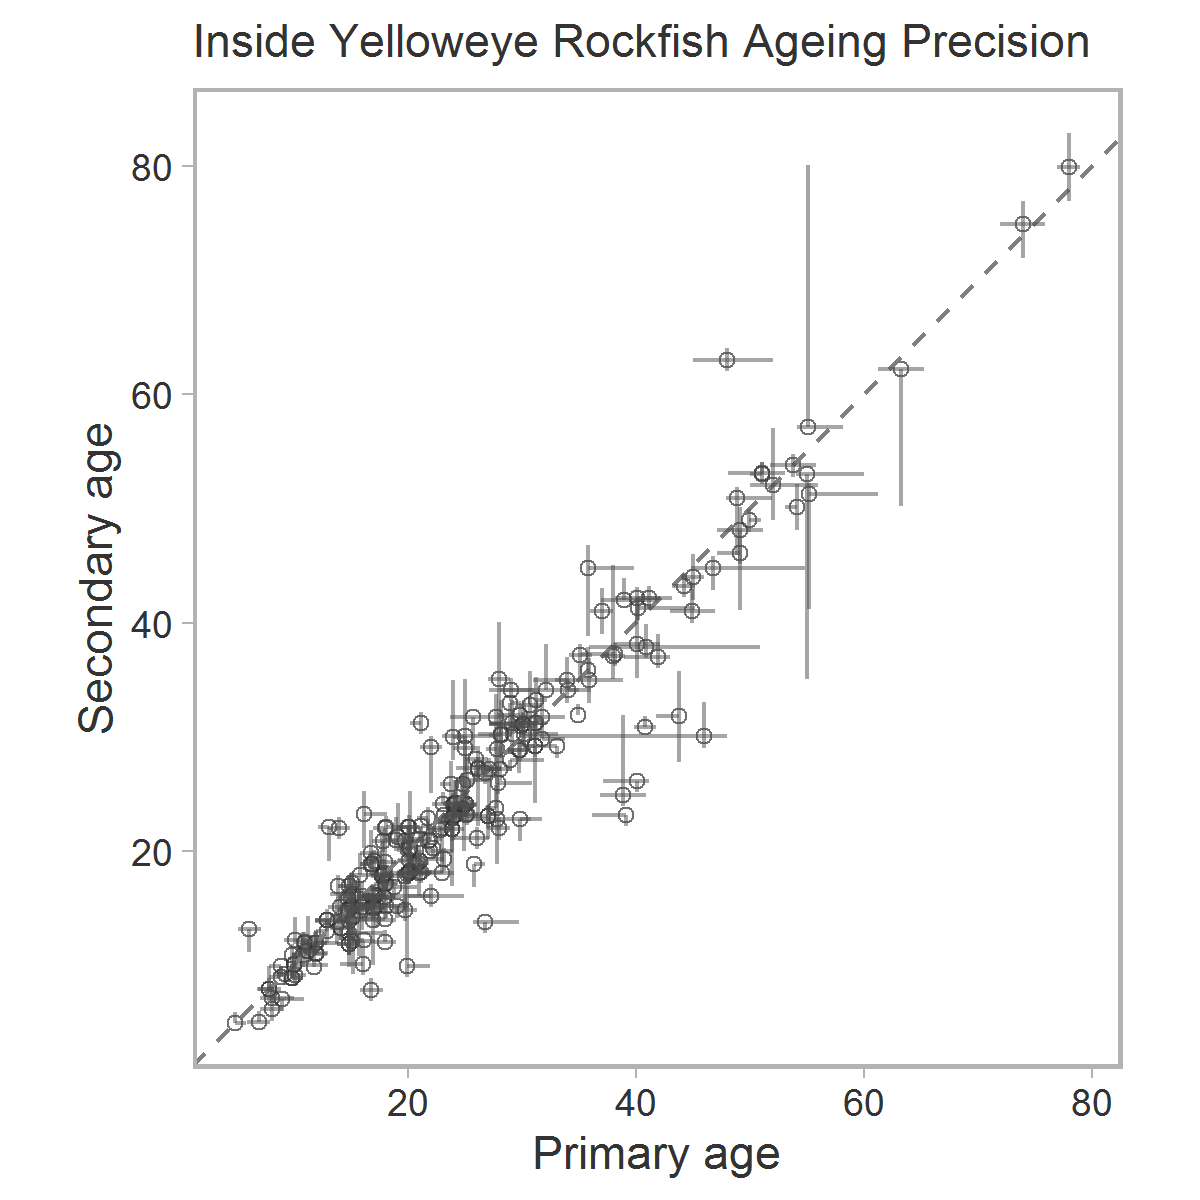
\includegraphics[width=4in]{C:/GitHub/yelloweye-inside/mse/figures-french/ye-ins-age-precision}}{Figure \ref{fig:age-precision}} 

}

\caption{Graphique de précision de la détermination de l'âge pour le sébaste aux yeux jaunes des eaux intérieures. Chaque point et hachure représente un poisson individuel dont l'âge a été déterminé deux fois. L'axe des abscisses représente l'âge et les extrémités supérieures et inférieures de la fourchette des âges possibles enregistrés par le premier lecteur (« principal ») de l'âge des poissons. L'axe des ordonnées représente les valeurs équivalentes enregistrées par le deuxième lecteur (« précision ») de l'âge du poisson. La ligne diagonale tiretée représente un parfait accord un à un entre les deux âges. Parmi tous les sébastes aux yeux jaunes dont l'âge a été déterminé avec précision, 300 poissons ont été échantillonnés au hasard et une petite quantité de fluctuation aléatoire a été ajoutée aux deux axes pour réduire la surreprésentation, la même valeur de fluctuation étant ajoutée aux axes x et y pour un poisson donné.}\label{fig:age-precision}
\end{figure}

\begin{figure}[htb]

{\centering \pdftooltip{\includegraphics[width=5in]{C:/GitHub/yelloweye-inside/mse/figures-french/length-freq}}{Figure \ref{fig:length-freq}} 

}

\caption{Graphiques de la fréquence des longueurs pour le sébaste aux yeux jaunes des eaux intérieures d'après tous les relevés accessibles menés dans la zone 4B~: relevés à la palangre sur fond dur (nord et sud) dans les eaux intérieures (RPFD INT N/S), relevés à la palangre sur fond dur dans les eaux extérieures (une petite partie de la zone 4B a été incluse dans ce relevé en 2014 et en 2016; RPFD EXT S) et relevés « AUTRES », comprenant les relevés à la turlutte de 1985 et de 1986 et un relevé au chalut de fond en 2005. Les poissons femelles sont représentés par des barres colorées et les poissons mâles sont représentés derrière par des barres gris clair. Le nombre total de poissons mesurés pour un relevé et une année donnés est indiqué dans le coin supérieur gauche de chaque graphique.}\label{fig:length-freq}
\end{figure}
\begin{figure}[htb]

{\centering \pdftooltip{\includegraphics[width=0.6\textwidth]{C:/GitHub/yelloweye-inside/mse/figures-french/length-weight}}{Figure \ref{fig:length-weight}} 

}

\caption{Ajustements et graphiques du modèle longueur-poids pour le sébaste aux yeux jaunes des eaux intérieures. Les ajustements du modèle pour les femelles sont indiqués par une ligne pleine noire, et les ajustements du modèle pour les mâles sont indiqués par une ligne grise tiretée. Le texte dans le graphique montre les estimations des paramètres, et les cercles gris ouverts représentent les poissons individuels auxquels les modèles sont ajustés. Tous les échantillons prélevés dans la zone 4B sont compris.}\label{fig:length-weight}
\end{figure}
\begin{figure}[htb]

{\centering \pdftooltip{\includegraphics[width=0.6\textwidth]{C:/GitHub/yelloweye-inside/mse/figures-french/vb}}{Figure \ref{fig:length-age}} 

}

\caption{Ajustements et graphiques du modèle longueur-âge pour le sébaste aux yeux jaunes des eaux intérieures. Les ajustements du modèle sont indiqués pour les femelles par une ligne pleine noire, pour les mâles par une ligne grise tiretée, et pour les sexes combinés par une ligne fine noire. Le texte montre les estimations des paramètres, et les cercles gris ouverts représentent les poissons individuels auxquels les modèles sont ajustés. Tous les échantillons de relevé sont compris.}\label{fig:length-age}
\end{figure}
\begin{figure}[htb]

{\centering \pdftooltip{\includegraphics[width=0.6\textwidth]{C:/GitHub/yelloweye-inside/mse/figures-french/mat-ogive-age}}{Figure \ref{fig:percent-maturity}} 

}

\caption{Courbes de l'âge à la maturité pour le sébaste aux yeux jaunes des eaux intérieures. Les lignes noires pleines représentent les ajustements aux poissons femelles et les lignes grises tiretées, les ajustements aux poissons mâles. Les lignes verticales indiquent l'âge estimé à 50 \% de maturité. Le texte dans les graphiques indique l'âge estimé à 5, 50 et 95 \% de maturité pour les femelles (F) et les mâles (M). Les traits courts en haut et en bas représentent jusqu'à 1 500 poissons choisis au hasard, avec une petite fluctuation aléatoire pour aider à différencier les poissons individuels.}\label{fig:percent-maturity}
\end{figure}

\begin{figure}[htb]

{\centering \pdftooltip{\includegraphics[width=0.6\textwidth]{C:/GitHub/yelloweye-inside/mse/figures-french/mat-prop}}{Figure \ref{fig:prop-mature}} 

}

\caption{Proportions prédites et observées de la maturité selon l'âge chez le sébaste aux yeux jaunes des eaux intérieures.}\label{fig:prop-mature}
\end{figure}

\begin{figure}[htb]

{\centering \pdftooltip{\includegraphics[width=0.6\textwidth]{C:/GitHub/yelloweye-inside/mse/figures-french/mat-months}}{Figure \ref{fig:mat-months}} 

}

\caption{Courbe de la fréquence de maturité par mois pour le sébaste aux yeux jaunes des eaux intérieures. La superficie de chaque cercle correspond au nombre de spécimens de poissons dans une catégorie de maturité donnée pour un mois donné. Les femelles sont indiquées par des cercles noirs et les mâles sont indiqués derrière par des cercles gris clair. Le nombre total de spécimens de poissons pour chaque mois est indiqué par les chiffres figurant en haut du graphique.}\label{fig:mat-months}
\end{figure}
\clearpage

\hypertarget{tableau-ruxe9capitulatif-des-donnuxe9es-biologiques-accessibles}{%
\appsection{TABLEAU RÉCAPITULATIF DES DONNÉES BIOLOGIQUES ACCESSIBLES}\label{tableau-ruxe9capitulatif-des-donnuxe9es-biologiques-accessibles}}
\begin{longtable}[]{@{}ccccccc@{}}
\caption{\label{tab:test}Données biologiques sur le sébaste aux yeux jaunes des eaux intérieures.}\tabularnewline
\toprule
Année & Spécimens & Longueurs & Poids & Maturités & Âges & Spécimens d'âge prélevés\tabularnewline
\midrule
\endfirsthead
\toprule
Année & Spécimens & Longueurs & Poids & Maturités & Âges & Spécimens d'âge prélevés\tabularnewline
\midrule
\endhead
1984 & 2 & 1 & 2 & 1 & 0 & 2\tabularnewline
1985 & 87 & 83 & 83 & 86 & 87 & 87\tabularnewline
1986 & 37 & 37 & 37 & 37 & 28 & 37\tabularnewline
1987 & 5 & 5 & 5 & 5 & 0 & 5\tabularnewline
1988 & 12 & 10 & 10 & 12 & 0 & 12\tabularnewline
1992 & 2 & 2 & 2 & 2 & 0 & 2\tabularnewline
1993 & 1 & 1 & 1 & 1 & 0 & 1\tabularnewline
2003 & 135 & 131 & 130 & 107 & 135 & 135\tabularnewline
2004 & 118 & 117 & 115 & 80 & 118 & 118\tabularnewline
2005 & 146 & 141 & 134 & 124 & 146 & 146\tabularnewline
2007 & 65 & 65 & 64 & 53 & 65 & 65\tabularnewline
2008 & 38 & 37 & 30 & 23 & 32 & 38\tabularnewline
2009 & 10 & 10 & 10 & 10 & 8 & 10\tabularnewline
2010 & 153 & 153 & 153 & 145 & 153 & 153\tabularnewline
2011 & 266 & 264 & 264 & 263 & 264 & 266\tabularnewline
2012 & 171 & 170 & 169 & 144 & 169 & 171\tabularnewline
2013 & 223 & 222 & 223 & 209 & 220 & 223\tabularnewline
2014 & 191 & 191 & 190 & 178 & 159 & 191\tabularnewline
2015 & 236 & 232 & 230 & 219 & 209 & 236\tabularnewline
2016 & 257 & 257 & 257 & 247 & 253 & 257\tabularnewline
2018 & 55 & 55 & 55 & 52 & 55 & 55\tabularnewline
\bottomrule
\end{longtable}
\clearpage


\clearpage

\refstepcounter{chapter}
\label{app:index-data}
\starredchapter{ANNEXE~\thechapter. DONNÉES DES RELEVÉS INDÉPENDANTES DE LA PÊCHE}

Nous avons conditionné les modèles opérationnels à l'aide d'indices de l'abondance tirés du relevé à la palangre sur fond dur (RPFD) et du relevé à la palangre sur l'aiguillat commun dans le détroit de Georgie. Les plans de relevé et la modélisation des indices connexes sont décrits ici.

\hypertarget{sec:hbll-index-data}{%
\appsection{INDICE DU RELEVÉ À LA PALANGRE SUR FOND DUR DANS LES EAUX INTÉRIEURES}\label{sec:hbll-index-data}}

Le relevé à la palangre sur fond dur dans les eaux intérieures pour la zone de gestion du détroit de Georgie (4B) fournit des indices des taux de prise et les données biologiques connexes pour l'évaluation du sébaste des zones côtières depuis 2003 (Lochead et Yamanaka \protect\hyperlink{ref-lochead2007}{2007}). Le relevé suit un plan stratification aléatoire de la profondeur qui consiste en blocs de 2 km par 2 km, et il a toujours été effectué par le NGCC Neocaligus. Le relevé utilise des hameçons circulaires de type agrafe de taille 13/0 et du calmar comme appât avec une durée d'immersion de deux heures. Les données hameçon par hameçon recueillies depuis le début des relevés sont collectées électroniquement et stockées dans une base de données. Pour plus de renseignements détaillés sur le plan du relevé, voir Lochead et Yamanaka (\protect\hyperlink{ref-lochead2004}{2004}).

La zone du relevé est divisée en régions du nord et du sud (figure~\ref{fig:map-HBLL-NS}), qui sont pêchées en alternance une année sur deux. La frontière entre les deux régions se situe approximativement aux extrémités nord des secteurs de gestion des pêches du Pacifique (SGPP) 14 et 15 (figure~\ref{fig:map-4B}). Cependant, plusieurs irrégularités se sont produites (figure~\ref{fig:hbll-raw})~:


\begin{figure}[htb]

{\centering \pdftooltip{\includegraphics[width=5in]{C:/GitHub/yelloweye-inside/figs/YE_Inside_2019_HBLL_L}}{Figure \ref{fig:map-HBLL-NS}} 

}

\caption{Carte des blocs du relevé à la palangre sur fond dur indiquant les régions du nord (en bleu) et du sud (en vert). Les aires de conservation du sébaste (blocs orange) sont également représentées.}\label{fig:map-HBLL-NS}
\end{figure}
\begin{itemize}

\item
  Le relevé n'a pas eu lieu en 2006 et en 2017.
\item
  La durée du relevé varie d'une année à l'autre, ce qui se traduit par des incohérences dans la portée géographique du relevé d'une année à l'autre.
\item
  La baie Desolation (SGPP 15) fait partie de la région du sud, mais a été échantillonnée dans la région du nord en 2003, 2008 et 2019, et ne l'a pas été en 2009 et 2018. Les taux de prise du sébaste aux yeux jaunes sont les plus élevés dans la baie Desolation (SGPP 15; figure~\ref{fig:map-4B}). Le manque d'échantillonnage en 2009 et en 2018 devrait donc avoir un effet sur les estimations du relevé du sud.
\item
  Le relevé du sud n'a pas été réalisé en entier en 2009; la pêche a seulement eu lieu dans 38 blocs dans le sud du détroit de Georgie, et uniquement entre Nanaimo et Victoria. Cela contraste avec les années normales où le relevé couvre environ 70 blocs jusqu'à Campbell River au nord. Les taux de prise de la plupart des espèces de sébastes capturées dans ce relevé ayant tendance à diminuer du nord au sud, cela pourrait également avoir un effet important sur l'indice du relevé cette année-là.
\end{itemize}
Nous avons appliqué un modèle spatiotemporel géostatistique pour normaliser l'indice du relevé à la palangre sur fond dur (p.~ex., Shelton et al. \protect\hyperlink{ref-shelton2014}{2014}; Thorson et al. \protect\hyperlink{ref-thorson2015}{2015}; Anderson et al. \protect\hyperlink{ref-anderson2019synopsis}{2019}) afin de tenir compte de la mise en œuvre irrégulière du plan du relevé (section~\ref{sec:hbll-spatiotemporal}). Nous avons confirmé, par simulation, que cette approche peut « assembler » les régions de relevé du nord et du sud avec relativement peu de biais (section~\ref{sec:hbll-sim}).

\hypertarget{sec:hbll-hook-competition}{%
\subsection{Concurrence à l'hameçon}\label{sec:hbll-hook-competition}}

Un indice de l'abondance d'une espèce tiré d'un relevé à la palangre n'est pas forcément proportionnel à l'abondance réelle dans certaines conditions. Par exemple, en cas de forte concurrence entre les espèces pour les hameçons appâtés, les prises réelles pourraient ne pas refléter fidèlement la véritable abondance des espèces moins compétitives (Kuriyama et al. \protect\hyperlink{ref-kuriyama2018}{2018}). Les prises du relevé à la palangre sur fond dur dans les eaux intérieures sont principalement composées d'aiguillat commun du Pacifique Nord (\emph{Squalus suckleyi}; ci-après « aiguillat commun »), un important concurrent potentiel des sébastes aux hameçons (Obradovich \protect\hyperlink{ref-obradovich2018}{2018}). Comme dans Yamanaka et al. (\protect\hyperlink{ref-yamanaka2011}{2011}), nous avons appliqué une correction de la concurrence à l'hameçon, qui tient compte de la concurrence entre les poissons individuels pour l'appât des hameçons, aux données du relevé à la palangre sur fond dur. Pour appliquer cette correction, on estime un facteur d'ajustement de la concurrence pour chaque calée, chaque année. Ce facteur d'ajustement, \(A_{i,t}\), met à l'échelle le nombre observé de sébastes aux yeux jaunes capturés, \(N_{i,t}\), pour chaque calée \(i\) chaque année \(t\) afin de donner le nombre prévu de poissons pêchés après la prise en compte de la concurrence, \(N_{i,t}^{(0)}\)~:
\begin{equation}
N_{i,t}^{(0)} = A_{i,t} N_{i,t}.
\label{eq:Nit}
\end{equation}
Le facteur d'ajustement dépend de la proportion d'hameçons observés qui sont remontés encore appâtés, \(P_{i,t}\) (figure~\ref{fig:hbll-baited})~:
\begin{equation}
A_{i,t} = – \frac{ \log P_{i,t}}{1 – P_{i,t}}.
\label{eq:hbll-hook-adjustment}
\end{equation}
Étant donné que \(P_{i,t} \rightarrow 0\), \(A_{i,t} \rightarrow \infty\), de sorte que le nombre prévu \(N_{i,t}^{(0)} \rightarrow \infty\). Par conséquent, dans les cas où aucun hameçon n'a été remonté encore appâté, nous avons fixé le nombre d'hameçons appâtés à un. Voir plus de renseignements détaillés sur la correction de la concurrence à l'hameçon dans Anderson et al. (\protect\hyperlink{ref-anderson2019synopsis}{2019}) (leur annexe G, section G.5). Nous avons entré les données ajustées en fonction de la concurrence à l'hameçon (figure~\ref{fig:hbll-hook-adjustment}) dans le modèle spatiotemporel pour développer l'indice de l'abondance.

\hypertarget{sec:hbll-spatiotemporal}{%
\subsection{Normalisation de l'indice spatiotemporel du relevé à la palangre sur fond dur}\label{sec:hbll-spatiotemporal}}

Nous avons ajusté un modèle de normalisation de l'indice spatiotemporel géostatistique~:
\begin{align}
  y_{s,t} &\sim \mathrm{NegBin}\left(\mu_{s,t}, \phi \right),\\
  \mu_{s,t} &= \exp \left( \bm{X}_{s,t} O_{s,t} + \bm{\beta} + \omega_s + \epsilon_{s,t} \right),
\label{eq:hbll-model}
\end{align}
où NegBin fait référence à la distribution binomiale négative (le paramétrage NB2 (Hilbe \protect\hyperlink{ref-hilbe2011}{2011}) où les échelles de la variance sont en quadrature avec la moyenne), \(\phi\) représente le paramètre de dispersion, \(y_{s,t}\) et \(\mu_{s,t}\) font référence à la valeur observée et prévue, respectivement, au point spatial \(s\) et dans le temps \(t\), \(\phi\) désigne le paramètre de dispersion, \(\bm{X}\) désigne une matrice du plan et \(\beta\) désigne un vecteur de coefficients estimés (une moyenne indépendante pour chaque année). Le symbole \(O_{s,t}\) représente une « compensation » pour le nombre d'hameçons et le facteur d'ajustement de la concurrence à l'hameçon. Plus précisément, il était représenté en tant que \(\log \left(S_{i,t} / A_{i,t} \right)\), où \(S_{i,t}\) représente la superficie « balayée » par la calée. Nous avons calculé la superficie balayée en fonction du nombre d'hameçons (\(N^\textrm{hooks}_{i,t}\)) dans la calée \(i\) et l'année \(t\) comme suit~:
\begin{equation}
N^\textrm{hooks}_{i,t} \cdot 0.0024384 \cdot 0.009144 \cdot 1000.
\end{equation}
La valeur 0,002438 correspond à l'espacement entre les hameçons (8 pouces) en kilomètres, 0,009144 à une superficie présumée de 30 pieds balayée autour de la calée où les poissons peuvent être capturés (en kilomètres) et 1 000 met à l'échelle la superficie balayée des kilomètres aux mètres. Il est à noter que l'hypothèse de 30 pieds ne sert qu'à augmenter ou à diminuer la densité pour toutes les années et a en fin de compte une incidence sur l'estimation de la capturabilité du relevé, mais n'influencera pas la forme des séries chronologiques de l'indice.

Nous avons supposé que les effets aléatoires spatiaux (\(\omega_s\)) étaient tirés d'une distribution normale multidimensionnelle avec une matrice de covariance \(\bm{\Sigma}_\omega\)~:
\begin{equation}
\bm{\omega} \sim \mathrm{MVNormal} \left( \bm{0}, \bm{\Sigma}_\omega \right).
\end{equation}
Nous avons limité les effets aléatoires spatiaux pour suivre une fonction de covariance de \mbox{Mat\'ern}, qui définit le taux de décroissance de la corrélation spatiale avec la distance. La fonction de \mbox{Mat\'ern} décrit la covariance \(\Phi_\omega \left( s_j, s_k \right)\) entre les emplacements spatiaux \(s_j\) et \(s_k\) comme suit~:
\begin{equation}
\Phi_\omega\left( s_j,s_k \right) = \tau_\omega^2/\Gamma(\nu)2^{\nu – 1}
    (\kappa d_{jk})^\nu K_\nu \left( \kappa d_{jk} \right),
\end{equation}
où \(\tau_\omega^2\) représente la variance spatiale, \(\Gamma\) représente la fonction gamma, \(K_\nu\) représente la fonction de Bessel, \(d_{jk}\) représente la distance euclidienne entre les emplacements \(s_j\) et \(s_k\), et \(\kappa\) représente un paramètre d'échelle estimé (p.~ex., Lindgren et al. \protect\hyperlink{ref-lindgren2011}{2011}). Le paramètre \(\nu\) contrôle le lissage de la fonction de covariance. Nous avons établi \(\nu = 1\), ce qui nous permet de tirer parti de l'approximation de l'équation différentielle partielle stochastique (SPDE) aux champs aléatoires de Markov gaussien (GMRF) pour augmenter considérablement l'efficacité de calcul (Lindgren et al. \protect\hyperlink{ref-lindgren2011}{2011}).

Nous avons supposé la même structure pour les effets aléatoires spatiotemporels, en attribuant à chaque tranche de temps son propre ensemble indépendant d'effets aléatoires (\(\bm{\epsilon}_t\)) avec la matrice de covariance \(\bm{\Sigma}_{\epsilon,t}\)~:
\begin{equation}
\bm{\epsilon}_t \sim \mathrm{MVNormal} \left( \bm{0}, \bm{\Sigma}_{\epsilon,t} \right).
\end{equation}
Cette matrice de covariance est également limitée pour suivre une fonction de covariance de \mbox{Mat\'ern} avec le même \(\kappa\), mais son propre \(\tau_\epsilon^2\) (variance spatiale)~:
\begin{equation}
\Phi_\epsilon\left( s_j,s_k \right) = \tau_\epsilon^2/\Gamma(\nu)2^{\nu – 1}
    (\kappa d_{jk})^\nu K_\nu \left( \kappa d_{jk} \right).
\end{equation}
Bien que nous ayons décrit les fonctions de \mbox{Mat\'ern} ci-dessus en utilisant la forme isométrique simple dans un souci de simplicité (la corrélation spatiale est la même dans toutes les directions), nous avons en fait autorisé l'anisotropie dans la corrélation spatiale et spatiotemporelle (p.~ex., Thorson et al. \protect\hyperlink{ref-thorson2015}{2015}).

Les effets aléatoires spatiaux tenaient compte de facteurs spatiaux qui étaient constants dans le temps, comme la profondeur et le type de substrat. Les effets aléatoires spatiotemporels intégraient des facteurs qui variaient d'une année à l'autre dans l'espace, comme la température au fond, les régimes de circulation de l'eau, les interactions entre espèces et les déplacements des espèces. À titre d'analyses de sensibilité, nous avons inclus d'autres versions de nos modèles qui 1) tenaient également compte de la profondeur et 2) ne tenaient pas compte de la concurrence à l'hameçon.

Nous avons ajusté notre modèle avec le progiciel sdmTMB en R (Anderson et al. \protect\hyperlink{ref-sdmtmb}{2020}\protect\hyperlink{ref-sdmtmb}{a}) et TMB (Kristensen et al. \protect\hyperlink{ref-tmb}{2016}) en utilisant un « maillage » avec 400 « nœuds » de processus prédictifs générés par des approximations de Laplace imbriquées et intégrées (INLA) (Lindgren et al. \protect\hyperlink{ref-lindgren2011}{2011}; Rue et al. \protect\hyperlink{ref-rue2016}{2016}) avec des emplacements déterminés par un algorithme de regroupement des K-moyennes (figure~\ref{fig:hbll-spde}). Nous avons estimé les effets fixes par vraisemblance maximale, les effets aléatoires étant fixés aux valeurs qui maximisaient la probabilité conjointe conditionnelle à la valeur estimée des effets fixes. Nous avons vérifié que les ajustements du modèle concordaient avec la convergence en nous assurant que le gradient maximal de tous les coefficients estimés était inférieur à 0,001 et que la matrice de covariance était positive-définie.

Nous avons projeté les prévisions du modèle sur toute la zone de relevé (figure~\ref{fig:hbll-area-grid}) à l'aide de la matrice de projection de covariance et du maillage d'interpolation bilinéaire fournis par INLA (Lindgren et al. \protect\hyperlink{ref-lindgren2011}{2011}; Rue et al. \protect\hyperlink{ref-rue2016}{2016}) (figures~\ref{fig:hbll-spde} et~\ref{fig:hbll-predicted-spacetime}). En ce qui concerne les composantes du modèle, les effets aléatoires spatiaux étaient, par définition, constants d'une année à l'autre (figure~\ref{fig:hbll-spatial-re}) et les effets aléatoires spatiotemporels variaient d'une année à l'autre (figure~\ref{fig:hbll-spatiotemporal-re}).

Nous avons alors calculé la biomasse prévue \(B_t\) pour l'année \(t\), comme suit~:
\begin{equation}
B_t = \sum_{j = 1}^{n_j}
  w_j \cdot \exp \left( \bm{X}_{j,t} \bm{\beta} + \bar{\bm{O}} + \omega_j + \epsilon_{j,t} \right),
\end{equation}
où \(j\) renvoie à une cellule du quadrillage dans la zone de relevé, \(w_j\) représente la superficie de cette cellule (figure~\ref{fig:hbll-area-grid}) et \(\bar{\bm{O}}\) représente la valeur de compensation moyenne. En d'autres termes, nous avons additionné la biomasse prévue pour chaque année dans toutes les cellules de quadrillage faisant partie de la zone de relevé. Nous avons généré les écarts­types pour les estimations annuelles de la biomasse logarithmique à l'aide de la méthode delta généralisée mise en œuvre dans Template Model Builder (Kristensen et al. \protect\hyperlink{ref-tmb}{2016}).

L'indice de la population normalisé ainsi obtenu tient compte de l'échantillonnage irrégulier de la zone de relevé et de la concurrence à l'hameçon et « assemble » les régions du nord et du sud en un seul indice de la population (figure~\ref{fig:hbll-index}). L'inclusion de la profondeur ou l'exclusion des ajustements de la concurrence à l'hameçon ont eu des effets relativement mineurs sur l'indice de la population (figure~\ref{fig:hbll-index}). Le modèle a également été en mesure de « remplir » ce à quoi l'indice pourrait ressembler hypothétiquement pour les régions du nord et du sud indépendamment (figure~\ref{fig:hbll-index}). Il convient de noter que cette interpolation statistique ne peut pas tenir compte d'événements ponctuels dans la région non observée, comme une abondance anormalement élevée seulement dans la région du nord une année où le relevé avait lieu dans la région du sud.

\hypertarget{sec:hbll-sim}{%
\subsection{Essais par simulation de « l'assemblage » des relevés par les modèles spatiotemporels}\label{sec:hbll-sim}}

Nous avons entrepris une analyse de simulation de base pour vérifier que notre approche « d'assemblage » des régions du nord et du sud dans une seule zone de relevé était raisonnable d'un point de vue statistique. Nous avons produit un système qui correspond approximativement aux données du relevé à la palangre sur fond dur avec lesquelles nous avons travaillé dans ce document~:
\begin{itemize}

\item
  10 ans d'observations
\item
  100 emplacements d'observation spatiale possibles, \(s_j\) et \(s_k\), tirés d'une distribution uniforme (0, 1) chaque année
\item
  Un ET marginal (\(\omega_s\)) = 2,2
\item
  Un ET marginal (\(\epsilon_{s,t}\)) = 0,3
\item
  Un paramètre de \mbox{Mat\'ern} \(\kappa = 0,1\)
\item
  Des moyennes annuelles tirées d'une distribution log-normale (0,1, 0,2)
\item
  Un processus d'observation de Poisson (dans un souci de simplicité plutôt qu'un binôme négatif)
\end{itemize}
Nous avons simulé l'abondance moyenne réelle sous-jacente sur un quadrillage complet {[}0, 1{]} contenant 25 x 25 cellules de taille égale. Nous avons ensuite rejeté les régions du nord et du sud (au-dessus ou en dessous de 0,5) en alternance une année sur deux, afin d'avoir environ 50 observations par année, et nous avons tenté d'ajuster la même forme de modèle spatiotemporel que celle utilisée pour la normalisation de l'indice du relevé à la palangre sur fond dur (figure~\ref{fig:stich-sim-pred}).

Même s'il n'observait que les régions du nord et du sud en alternance, le modèle a été en mesure de reconstituer les parties manquantes non observées à partir de la corrélation spatiale estimée et, dans une moindre mesure, de la corrélation spatiotemporelle estimée (figure~\ref{fig:stich-sim-pred}). En projetant les prévisions du modèle sur un quadrillage de toute la superficie du carré simulé, notre modèle a pu produire un indice semblable à l'indice réel (figure~\ref{fig:stich-sim-index}). Si nous générions plutôt l'indice de façon naïve en utilisant une approche qui imite une approche fondée sur le plan (en additionnant les abondances observées chaque année et en l'ajustant à la même moyenne géométrique à des fins de visualisation), l'indice obtenu ne reflétait pas la tendance de l'indice réel pour beaucoup d'années (figure~\ref{fig:stich-sim-index}).

Grâce à l'expérimentation (non illustrée), nous avons constaté que « l'assemblage » était le plus exact pour récupérer l'indice réel si l'ampleur des écarts de la corrélation spatiale (\(\omega_s\)) était beaucoup plus grande que celle des écarts de la corrélation spatiotemporelle (\(\epsilon_{s,t}\)). C'est le cas dans notre modèle de relevé à la palangre sur fond dur, où l'écart-type marginal de \(\omega_s\) était environ six fois plus grand que l'écart-type marginal de \(\epsilon_{s,t}\). « L'assemblage » était le plus nécessaire lorsque l'abondance présentait un gradient nord-sud, comme cela semble évident pour le sébaste aux yeux jaunes.
\begin{figure}[htb]

{\centering \pdftooltip{\includegraphics[width=\textwidth]{C:/GitHub/yelloweye-inside/figs-french/hbll-joint-raw-data}}{Figure \ref{fig:hbll-raw}} 

}

\caption{Observations de sébaste aux yeux jaunes dans le relevé à la palangre sur fond dur dans les eaux intérieures. L’arrière-plan ombré en gris indique les zones de relevé du nord et du sud. La superficie des cercles représente le nombre de poissons capturés par hameçon après prise en compte de la concurrence à l’hameçon.}\label{fig:hbll-raw}
\end{figure}
\begin{figure}[htb]

{\centering \pdftooltip{\includegraphics[width=5in]{C:/GitHub/yelloweye-inside/figs-french/hbll-area-in-water}}{Figure \ref{fig:hbll-area-grid}} 

}

\caption{Superficie par cellule de quadrillage du relevé qui se trouve dans l’eau pour le relevé à la palangre sur fond dur dans les eaux intérieures. La densité de comptage prévue pour chaque cellule du quadrillage est étendue à toute la zone de relevé en fonction de ces régions.}\label{fig:hbll-area-grid}
\end{figure}
\begin{figure}[htb]

{\centering \pdftooltip{\includegraphics[width=\textwidth]{C:/GitHub/yelloweye-inside/figs-french/hbll-joint-baited}}{Figure \ref{fig:hbll-baited}} 

}

\caption{Proportion d’hameçons appâtés remontés pour le relevé à la palangre sur fond dur dans les eaux intérieures. Il convient de noter la différence importante entre les régions du nord et du sud et le changement dans le nord entre 2003 et 2007 et les années suivantes.}\label{fig:hbll-baited}
\end{figure}
\begin{figure}[htb]

{\centering \pdftooltip{\includegraphics[width=\textwidth]{C:/GitHub/yelloweye-inside/figs-french/hbll-joint-hook-adjust}}{Figure \ref{fig:hbll-hook-adjustment}} 

}

\caption{Facteur d’ajustement des hameçons pour le relevé à la palangre sur fond dur dans les eaux intérieures, tenant compte du nombre d’hameçons et du nombre d’hameçons remontés appâtés.}\label{fig:hbll-hook-adjustment}
\end{figure}
\begin{figure}[htb]

{\centering \pdftooltip{\includegraphics[width=0.6\textwidth]{C:/GitHub/yelloweye-inside/figs-french/hbll-joint-spde}}{Figure \ref{fig:hbll-spde}} 

}

\caption{Maillage de l’équation différentielle partielle stochastique (SPDE) pour le relevé à la palangre sur fond dur. Les cercles gris ouverts en arrière-plan (souvent masqués) représentent les emplacements des données observées et les points rouges représentent les "knots". Les lignes indiquent le maillage de triangularisation utilisé dans l’approximation de l’équation différentielle partielle stochastique et l’interpolation bilinéaire. Un plus grand nombre de nœuds augmente la précision de l’approximation au détriment du temps de calcul.}\label{fig:hbll-spde}
\end{figure}
\begin{figure}[htb]

{\centering \pdftooltip{\includegraphics[width=\textwidth]{C:/GitHub/yelloweye-inside/figs-french/hbll-joint-prediction-log}}{Figure \ref{fig:hbll-predicted-spacetime}} 

}

\caption{Densité relative prédite dans l’espace et le temps pour le relevé à la palangre sur fond dur. Les nombres observés (avec ajustement des hameçons) sont illustrés par des cercles. Les prédictions sont illustrées par des ombres de couleur.}\label{fig:hbll-predicted-spacetime}
\end{figure}
\begin{figure}[htb]

{\centering \pdftooltip{\includegraphics[width=4.2in]{C:/GitHub/yelloweye-inside/figs-french/hbll-joint-omega}}{Figure \ref{fig:hbll-spatial-re}} 

}

\caption{Les effets spatiaux aléatoires. Il s’agit de différences constantes spatialement corrélées dans l’abondance prévue au fil du temps. Les valeurs sont indiquées dans l’espace des liens (log).}\label{fig:hbll-spatial-re}
\end{figure}
\begin{figure}[htb]

{\centering \pdftooltip{\includegraphics[width=\textwidth]{C:/GitHub/yelloweye-inside/figs-french/hbll-joint-epsilon}}{Figure \ref{fig:hbll-spatiotemporal-re}} 

}

\caption{Les effets aléatoires spatiotemporels. Il s’agit d’écarts spatialement corrélés qui changent dans le temps. Noter le retour à la moyenne dans les combinaisons superficie-année sans données d’échantillonnage. Noter la différence d’ampleur entre les effets aléatoires spatiaux (figure précédente) et ces effets aléatoires spatiotemporels.}\label{fig:hbll-spatiotemporal-re}
\end{figure}
\begin{figure}[htb]

{\centering \pdftooltip{\includegraphics[width=4in]{C:/GitHub/yelloweye-inside/figs-french/hbll-index-components-eps-depth2}}{Figure \ref{fig:hbll-index}} 

}

\caption{L’indice commun de l’abondance relative. Le graphique du haut illustre la prédiction commune à partir du modèle spatial temporel. Trois versions sont incluses~: 1) les effets aléatoires et les moyennes annuelles seulement, 2) l’ajout d’une covariable de profondeur et 3) l’élimination du facteur d’ajustement des hameçons. Les graphiques du milieu et du bas représentent les prévisions communes pour les régions du nord et du sud. Toutes les régions ombrées représentent des intervalles de confiance de 95\%. Les séries chronologiques des indices communs du graphique du haut ont été mises à l’échelle pour avoir la même moyenne géométrique que le principal indice ``RPFD INT'' à des fins de visualisation. Les lignes verticales tiretées indiquent les années où des relevés ont été effectués (surtout) dans la région du sud.}\label{fig:hbll-index}
\end{figure}
\clearpage
\begin{figure}[htb]

{\centering \pdftooltip{\includegraphics[width=\textwidth]{C:/GitHub/yelloweye-inside/figs-french/geostatistical-sim-predicted}}{Figure \ref{fig:stich-sim-pred}} 

}

\caption{Essais par simulation du calcul de l’indice de l’abondance relative avec des observations en alternance pour le nord et le sud. (A) L’abondance réelle simulée (moyenne) dans l’espace et dans le temps. (B) Les nombres observés (points) et estimés (couleurs) dans l’espace et le temps à partir du modèle géostatistique. Les observations se font en alternance une année sur deux dans les régions du nord et du sud et « omettent » la région manquante. Noter comment le modèle temporel spatial est capable de prédire ce que devrait être l’abondance dans la région « omise » en fonction du profil de la corrélation spatiale constante (et, dans une moindre mesure, le profil de la corrélation spatiotemporelle).}\label{fig:stich-sim-pred}
\end{figure}
\clearpage
\begin{figure}[htb]

{\centering \pdftooltip{\includegraphics[width=5in]{C:/GitHub/yelloweye-inside/figs-french/geostatistical-sim-stitched-index}}{Figure \ref{fig:stich-sim-index}} 

}

\caption{Essais par simulation du calcul de l’indice de l’abondance relative avec des observations en alternance pour le nord et le sud. La ligne rouge pleine représente l’abondance réelle simulée dans le temps. La ligne pointillée et tiretée verte représente une estimation « naïve » fondée sur le plan, qui est calculée ici en calculant l’abondance avec seulement les nombres du nord ou du sud observés chaque année. La ligne bleue tiretée représente un indice géostatistique normalisé qui tente de tenir compte des observations biennales nord-sud. La région bleue ombrée représente l’intervalle de confiance de 95\% modélisé.}\label{fig:stich-sim-index}
\end{figure}
\clearpage

\hypertarget{sec:dogfish-index-data}{%
\appsection{INDICE DU RELEVÉ SUR L'AIGUILLAT COMMUN}\label{sec:dogfish-index-data}}

Le relevé sur l'aiguillat commun échantillonne neuf emplacements dans le détroit de Georgie qui ont été historiquement exploités par la pêche commerciale de l'espèce (King et al. \protect\hyperlink{ref-king2012}{2012}). Le relevé a commencé en 1986 et l'échantillonnage a eu lieu en 1989, 2005, 2011, 2014 et 2019. Il s'agit d'un relevé à la palangre stratifié en profondeur qui utilise des engins à agrafe avec 300 hameçons circulaires de taille 14/0 appâtés avec du hareng du Pacifique et une durée d'immersion de deux heures. Une description plus détaillée des méthodes de relevé est donnée dans King et al. (\protect\hyperlink{ref-king2012}{2012}). Pour la plupart des séries chronologiques, les prises de sébaste ont été enregistrées calée par calée. Depuis 2019, des données hameçon par hameçon pour toutes les espèces capturées ont été recueillies à bord, ainsi que les données biologiques pour le sébaste. Nous utilisons un modèle spatiotemporel pour estimer la densité du sébaste aux yeux jaunes par km\textsuperscript{2}. Nous avons calculé la superficie balayée en multipliant le nombre d'hameçons déployés par la distance estimée entre les hameçons (espacement de 8 pieds) et la largeur balayée estimée (longueur de deux avançons).

Le relevé sur l'aiguillat commun n'est pas conçu pour évaluer le sébaste, de sorte qu'il y a plusieurs différences importantes entre les plans des relevés à la palangre sur fond dur et sur l'aiguillat commun. La différence la plus importante est peut-être que le relevé à la palangre sur fond dur cible en particulier les habitats propices au sébaste (c.-à-d.~un fond dur), tandis que le relevé sur l'aiguillat commun est effectuée dans des sites qui étaient importants pour la pêche commerciale et qui présentent principalement des fonds de sédiments meubles. Le relevé sur l'aiguillat commun utilise également des hameçons circulaires légèrement plus gros que ceux utilisés pour le relevé à la palangre sur fond dur (14/0 par rapport à 13/0); des appâts de hareng au lieu de calmar; 300 hameçons par calée au lieu de 225; et les hameçons sont espacés de 1,8 mètre au lieu de 2,4 mètres. Nous utilisons le relevé sur l'aiguillat commun dans cette analyse parce qu'il fournit la plus longue série chronologique de données indépendantes de la pêche pour le sébaste aux yeux jaunes des eaux intérieures et parce qu'il a été utilisé dans l'évaluation précédente en 2011.

\hypertarget{sec:dog-hook-comparison}{%
\subsection{Comparaison des hameçons}\label{sec:dog-hook-comparison}}

À l'origine, le relevé était effectué avec des hameçons en J, puis on les a remplacés par des hameçons circulaires en 2005. En 2004, McFarlane et al. (\protect\hyperlink{ref-mcfarlane2005}{2005}) ont entrepris une étude d'étalonnage pour évaluer la possibilité de modifier les taux de prise en raison du changement du type d'hameçon. Toutefois, l'étude a comparé les taux de prise pour l'aiguillat commun seulement, et le changement d'hameçon a probablement eu une incidence différente sur la capturabilité pour le sébaste aux yeux jaunes. L'évaluation précédente a tenté de régler ce problème en estimant un ratio de capturabilité, en utilisant les données pour tous les sébastes, afin d'évaluer les prises dans les années 1980 (Yamanaka et al. \protect\hyperlink{ref-yamanaka2011}{2011}). Leur description n'explique pas clairement comment ce ratio de capturabilité a été estimé. L'évaluation précédente était très sensible à l'indice de l'aiguillat commun obtenu (en raison de la forte diminution depuis les années 1980), et cette diminution dépendait en grande partie du ratio des hameçons.

Dans l'étude de comparaison des hameçons, \text{23} calées utilisaient des hameçons circulaires et \text{23} des hameçons en J. Dans ces calées expérimentales, \text{5} sébastes aux yeux jaunes ont été capturés à l'aide d'hameçons en J et \text{27} à l'aide d'hameçons circulaires (tableau~\ref{tab:dogfish-hook-comparison}). Bien que cela représente un échantillon relativement petit de poissons pour estimer un facteur de correction des hameçons pour le sébaste aux yeux jaunes, en estimant simultanément le facteur de correction tout en normalisant l'indice de la population à l'aide d'un modèle géostatistique, nous avons été en mesure d'intégrer l'incertitude du facteur de correction dans les erreurs types de l'indice ainsi obtenues (section~\ref{sec:dog-index-model}). Néanmoins, il est important de noter que ce facteur de correction est basé sur un nombre limité de calées. Il repose principalement sur cinq calées avec un ou deux sébastes aux yeux jaunes de plus capturés au moyen d'hameçons circulaires que par des hameçons en J et deux calées avec 12 et quatre sébastes aux yeux jaunes capturés au moyen d'hameçons circulaires contre zéro au moyen d'hameçons en J (tableau~\ref{tab:dogfish-hook-comparison}).

\clearpage
\begin{longtable}[]{@{}rrr@{}}
\caption{\label{tab:dogfish-hook-comparison}Nombre de sébastes aux yeux jaunes capturés dans l'expérience hameçon en J/hameçon circulaire en 2004.}\tabularnewline
\toprule
Calée & Hameçon en J & Hameçon circulaire\tabularnewline
\midrule
\endfirsthead
\toprule
Calée & Hameçon en J & Hameçon circulaire\tabularnewline
\midrule
\endhead
1 & 0 & 0\tabularnewline
2 & 0 & 1\tabularnewline
3 & 0 & 0\tabularnewline
4 & 0 & 0\tabularnewline
5 & 0 & 2\tabularnewline
6 & 0 & 0\tabularnewline
7 & 1 & 1\tabularnewline
8 & 0 & 0\tabularnewline
9 & 1 & 0\tabularnewline
10 & 0 & 0\tabularnewline
11 & 0 & 12\tabularnewline
12 & 0 & 0\tabularnewline
13 & 0 & 2\tabularnewline
14 & 0 & 0\tabularnewline
15 & 0 & 0\tabularnewline
16 & 0 & 0\tabularnewline
17 & 0 & 1\tabularnewline
18 & 0 & 4\tabularnewline
19 & 0 & 0\tabularnewline
20 & 0 & 0\tabularnewline
21 & 0 & 0\tabularnewline
22 & 0 & 0\tabularnewline
23 & 3 & 4\tabularnewline
\bottomrule
\end{longtable}
\hypertarget{sec:dog-depth}{%
\subsection{Profondeur}\label{sec:dog-depth}}

Outre le fait que le relevé n'a pas été conçu pour les sébastes et du changement de type d'engin, la strate de plus faible profondeur a été abandonnée dans le relevé de 2004 et les suivants. L'objectif était de délibérément essayer d'éviter de capturer les sébastes (pour des raisons de conservation). Bien que la profondeur ne soit pas explicitement incluse dans le modèle spatiotemporel, les effets spatiaux aléatoires devraient absorber une grande partie de la variation associée à la profondeur tout en tenant compte d'autres effets spatialement variables.

\hypertarget{sec:dog-hook-competition}{%
\subsection{Concurrence à l'hameçon}\label{sec:dog-hook-competition}}

L'évaluation précédente du sébaste aux yeux jaunes des eaux intérieures indique qu'un modèle exponentiel de concurrence à l'hameçon a été utilisé sur les données du relevé sur l'aiguillat commun en 2011. Toutefois, il n'y a pas de données accessibles sur le nombre d'hameçons appâtés et vides pour le relevé sur l'aiguillat commun avant 2019, et on ne sait pas bien comment l'évaluation précédente en a tenu compte. Par conséquent, nous n'avons pas appliqué un modèle explicite de concurrence à l'hameçon dans la présente analyse. Cependant, pour tenir compte en partie de la concurrence à l'hameçon, nous avons inclus le nombre d'aiguillats communs capturés (log-transformé de façon à avoir un effet multiplicateur sur le nombre observé) comme covariable dans le modèle.

\hypertarget{sec:dog-index-model}{%
\subsection{Normalisation de l'indice spatiotemporel du relevé sur l'aiguillat commun}\label{sec:dog-index-model}}

Nous avons utilisé un modèle géostatistique semblable à celui décrit pour le relevé à la palangre sur fond dur (section~\ref{sec:hbll-spatiotemporal}) avec l'ajout des covariables de l'aiguillat commun et du type d'hameçon. Nous avons inclus le nombre logarithmique d'aiguillats communs et le type d'hameçon dans la matrice du modèle \(\bm{X}_{s,t}\)~:
\begin{align}
  y_{s,t} &\sim \mathrm{NegBin}(\mu_{s,t}, \phi),\\
  \mu_{s,t} &= \exp \left( \bm{X}_{s,t} \bm{\beta} + O_{s,t} + \omega_s + \epsilon_{s,t} \right),
\label{eq:dogfish-model}
\end{align}
avec les symboles définis comme dans l'équation~\ref{eq:hbll-model}. Le type d'hameçon est un identificateur pour différencier les hameçons en J des hameçons circulaires. Le décalage représente le log(superficie balayée), tel que défini précédemment. Nous avons ajusté notre modèle avec sdmTMB (Anderson et al. \protect\hyperlink{ref-sdmtmb}{2020}\protect\hyperlink{ref-sdmtmb}{a}) tel que décrit ci-dessus avec 300 nœuds. Dans notre projection des prévisions du modèle sur le quadrillage du relevé pour calculer l'abondance relative normalisée~:
\begin{equation}
B_t = \sum_{j = 1}^{n_j}
  w_j \cdot \exp \left( \bm{X}_{j,t} \bm{\beta} + \bar{\bm{O}} + \omega_j + \epsilon_{j,t} \right),
\label{eq:dog-prediction}
\end{equation}
avec les symboles définis ci-dessus, nous avons pu faire des prédictions pour un hameçon en J ou un hameçon circulaire. Le choix de l'un ou de l'autre placerait davantage l'incertitude dans les années avec l'un ou l'autre puisque l'incertitude de l'autre effet ne serait incorporée que certaines années. En guise de compromis, nous avons choisi de faire des prédictions pour un type d'hameçon moyen dans l'ensemble de données afin de répartir l'incertitude de ce type dans les séries chronologiques. Dans la pratique, cela signifiait un codage de \text{-0,57} pour les hameçons circulaires et de \text{0,43} pour les hameçons en J dans la matrice d'ajustement du modèle \(\bm{X}_{s,t}\) et de fixer à 0 le prédicteur équivalent dans la matrice du modèle de prédiction.

Nous avons estimé que les hameçons en J capturaient 7,7 fois plus de sébastes aux yeux jaunes que les hameçons circulaires, toutes choses étant égales par ailleurs, mais avec une incertitude considérable (intervalle de confiance (IC) de 95 \%~: 1,6 -- 37,1). Nous avons estimé que l'effet de logarithme pour l'aiguillat commun était de -0,31 (IC de 95 \%~: -0,59 -- -0,03). Cela signifie que nous pouvons nous attendre à capturer, en moyenne, environ \text{3,1}\% (IC de 95 \%~: \text{0,3}\% -- \text{5,9}\%) moins de sébaste aux yeux jaunes pour chaque tranche supplémentaire de 10 \% d'aiguillat commun également pêché dans la même calée, probablement en raison de la concurrence à l'hameçon.

Dans l'équation~\ref{eq:dog-prediction}, nous avons organisé les cellules du quadrillage de prédiction, indexées par \(j\), en superposant un quadrillage de 500 mètres x 500 mètres sur la zone de relevé. Étant donné que le relevé sur l'aiguillat commun utilise des stations fixes plutôt qu'un quadrillage d'échantillonnage aléatoire, nous avons tracé manuellement des rectangles autour de toutes les calées de palangres exploitées historiquement afin de délimiter la zone échantillonnée (figure~\ref{fig:dog-raw}). Nous avons calculé la superficie des cellules du quadrillage (\(w_j\)) après avoir enlevé une partie des cellules à échelle fine qui chevauchaient les terres. Nous avons établi la matrice du plan \(\bm{X}_{j,t}\) pour prédire un nombre moyen d'aiguillats communs et un décalage moyen de la superficie balayée.

La projection résultante du modèle sur la grille à échelle fine est illustrée sur la figure~\ref{fig:dog-prediction} ainsi que les valeurs modélisées des effets aléatoires spatiaux (figure~\ref{fig:dog-spatial}) et spatiotemporels (figure~\ref{fig:dog-spatiotemporal}). L'indice normalisé pour le sébaste aux yeux jaunes pour un type d'hameçon moyen indique une diminution de l'abondance relative entre les années 1980 et le relevé suivant en 2004, mais avec une incertitude considérable (figure~\ref{fig:dog-standardized-index}). L'indice est demeuré relativement stable de 2004 à 2014, avec une légère augmentation de la moyenne de 2014 à 2019, mais encore une fois avec une incertitude considérable (figure~\ref{fig:dog-standardized-index}).

\clearpage
\begin{figure}[htb]

{\centering \pdftooltip{\includegraphics[width=\textwidth]{C:/GitHub/yelloweye-inside/figs-french/dogfish-yelloweye-per-area-data}}{Figure \ref{fig:dog-raw}} 

}

\caption{Sébastes aux yeux jaunes capturés, par zone balayée, par des hameçons dans le relevé sur l’aiguillat commun. Les valeurs sont indiquées par la superficie des cercles. Les rectangles gris illustrent la zone de relevé présumée.}\label{fig:dog-raw}
\end{figure}
\begin{figure}[htb]

{\centering \pdftooltip{\includegraphics[width=\textwidth]{C:/GitHub/yelloweye-inside/figs-french/dogfish-prediction-log}}{Figure \ref{fig:dog-prediction}} 

}

\caption{Abondance relative prédite du sébaste aux yeux jaunes (couleur). L’échelle de couleurs est log-transformée. Les cercles représentent les mêmes données observées que sur la figure précédente.}\label{fig:dog-prediction}
\end{figure}
\begin{figure}[htb]

{\centering \pdftooltip{\includegraphics[width=4.2in]{C:/GitHub/yelloweye-inside/figs-french/dogfish-omega}}{Figure \ref{fig:dog-spatial}} 

}

\caption{Effets aléatoires spatiaux du modèle spatiotemporel représentés dans l’espace logarithmique. Ce graphique représente une corrélation spatiale constante dans le temps.}\label{fig:dog-spatial}
\end{figure}
\begin{figure}[htb]

{\centering \pdftooltip{\includegraphics[width=\textwidth]{C:/GitHub/yelloweye-inside/figs-french/dogfish-epsilon}}{Figure \ref{fig:dog-spatiotemporal}} 

}

\caption{Effets aléatoires spatiotemporels du modèle spatiotemporel représentés dans l’espace logarithmique. Ces graphiques représentent une corrélation spatiale qui varie dans le temps.}\label{fig:dog-spatiotemporal}
\end{figure}
\begin{figure}[htb]

{\centering \pdftooltip{\includegraphics[width=5in]{C:/GitHub/yelloweye-inside/figs-french/dogfish-index-estimated-hook}}{Figure \ref{fig:dog-standardized-index}} 

}

\caption{L’indice normalisé de l’abondance relative du sébaste aux yeux jaunes ainsi obtenu. Les points représentent les estimations moyennes et les segments linéaires représentent les intervalles de confiance de 95\%. La ligne verticale tiretée représente l’année de l’expérience avec les hameçons et le passage des hameçons en J aux hameçons circulaires.}\label{fig:dog-standardized-index}
\end{figure}
\clearpage


\clearpage

\refstepcounter{chapter}
\label{app:catch-data}
\starredchapter{ANNEXE~\thechapter. DONNÉES SUR LES PRISES}

Le sébaste aux yeux jaunes des eaux intérieures est ciblé dans les pêches commerciales à la ligne et à l'hameçon, les pêches à des fins alimentaires, sociales et rituelles (ASR) et les pêches récréatives. La gestion de la pêche du sébaste aux yeux jaunes des eaux intérieures a commencé en 1986, avec la mise en place du permis commercial de catégorie « ZN » et des limites de prises quotidiennes pour les pêcheurs récréatifs. Une chronologie des changements de gestion pour les pêches commerciales et récréatives est présentée dans les tableaux~\ref{tab:comm-mgt-changes} et~\ref{tab:rec-mgt-changes}.

\hypertarget{sec:com-catch-data}{%
\appsection{DONNÉES SUR LES PRISES COMMERCIALES}\label{sec:com-catch-data}}

Les données sur les prises de sébaste peuvent être regroupées en trois périodes~: historique (de 1918 à 1950), début de la période électronique (de 1951 à 2005) et moderne (2006 et après). Il y a deux grandes sources d'incertitude dans la période historique et le début de la période électronique pour le sébaste aux yeux jaunes des eaux intérieures. La première est que les prises de sébastes, autres que de sébaste à longue mâchoire (\emph{Sebastes alutus}), étaient déclarées de façon regroupée (autre sébaste, ORF) pendant la période historique. Pour reconstituer les prises historiques, des auteurs du MPO ont élaboré un algorithme (Haigh et Yamanaka \protect\hyperlink{ref-haigh2011}{2011}). Cet algorithme de reconstitution applique un ratio calculé à partir d'une période pour laquelle on dispose de données crédibles sur les débarquements provenant du programme de vérification à quai des pêches à la ligne et à l'hameçon (1997--2005) pour générer une série chronologique des prises par espèce, année, secteur de pêche et zone de gestion (Haigh et Yamanaka \protect\hyperlink{ref-haigh2011}{2011}). Les données « crédibles » sur les débarquements sont tirées des années de référence où la connaissance des prises était considérée comme étant de grande qualité et stable, depuis 1997, avec le début de la présence d'observateurs à bord des chalutiers et le système de quotas individuels des bateaux (Haigh et Yamanaka \protect\hyperlink{ref-haigh2011}{2011}).

La deuxième grande source d'incertitude est l'ampleur des prises non déclarées qui étaient remises à l'eau ou rejetées en mer avant la mise en place du niveau de présence des observateurs de 100 \% en 2006. La reconstitution des prises de Haigh et Yamanaka (\protect\hyperlink{ref-haigh2011}{2011}) suppose qu'il n'y avait pas de rejet avant 1986, année où le permis ZN a été institué. On suppose qu'auparavant, tous les sébastes étaient conservés. Les rejets sont présumés être entièrement déclarés dans les bases de données du MPO depuis 2006 et le niveau de présence des observateurs en mer de 100 \%. Les prises de sébaste aux yeux jaunes non conservées (remises à l'eau ou rejetées) ont été estimées pour chaque pêche à l'aide du ratio des rejets de sébaste aux yeux jaunes par les cibles de débarquement propres à la pêche d'après les données de 2000 à 2004 des registres des observateurs des pêches à la ligne et à l'hameçon. Les prises historiques non déclarées ont ensuite été intégrées à la reconstitution des prises, pour donner un total annuel final.

La série chronologique des prises commerciales utilisée dans cette analyse (figure~\ref{fig:commcatch2} et tableau~\ref{tab:commcatch}) diffère de celle précédemment présentée en 2009 pour plusieurs raisons. Le contrôle continu de la qualité et les mises à jour de la base de données sur les prises de poisson de fond ont entraîné des différences mineures dans les données au fil du temps (Maria Surry, MPO, Station biologique du Pacifique, comm. pers., 9 mars 2020). De plus, une version antérieure de l'algorithme de reconstitution des prises a été utilisée pour élaborer la série chronologique pour l'évaluation des stocks précédente, car la version finale n'avait pas encore été publiée. D'autres améliorations apportées à l'algorithme de reconstitution ont provoqué des changements importants des prises historiques estimées certaines années (Norm Olsen, MPO, Station biologique du Pacifique, comm. pers., 9 mars 2020).

L'algorithme de reconstitution aurait pu être appliqué à toutes les années de la série chronologique jusqu'en 2005 (après quoi la vérification complète en mer et à quai est entrée en vigueur). Toutefois, pour cette analyse, nous avons utilisé les données reconstituées sur les prises de 1918 à 1985 et nous sommes passés aux données sur les prises nominales en 1986. Les prises nominales de 1986 à 2005 ont ensuite été doublées, conformément à l'évaluation précédente (Yamanaka et al. \protect\hyperlink{ref-yamanaka2011}{2011}). Nous avons choisi de doubler les prises nominales plutôt que les prises reconstituées parce que, avant l'évaluation précédente, les représentants de l'industrie nous avaient dit qu'ils n'avaient pas confiance dans la reconstitution des prises entre 1986 et 2005 et que l'échelle des prises non déclarées était probablement égale aux prises débarquées (DFO \protect\hyperlink{ref-dfo2012b}{2012}\protect\hyperlink{ref-dfo2012b}{b}). Ces indications nous ont amenés à doubler les prises pour ces années (Yamanaka et al. \protect\hyperlink{ref-yamanaka2011}{2011}). Cependant, comme les rejets sont estimés dans le cadre de l'algorithme de reconstitution des prises, dans l'analyse actuelle, nous avons doublé les prises nominales pour la période 1986--2005 (plutôt que les prises reconstituées) afin d'éviter de compter les rejets deux fois. Pour vérifier la sensibilité, nous explorons un scénario de modèle opérationnel où les prises commerciales de 1986 à 2005 n'ont pas été doublées (le scénario « Prises faibles » (2), section~\ref{sec:approach3-reference2}).
\begin{figure}[htb]

{\centering \pdftooltip{\includegraphics[width=0.8\textwidth]{knitr-figs-pdf/commcatch2-1}}{Figure \ref{fig:commcatch2}} 

}

\caption{Prises commerciales par secteur pour le sébaste aux yeux jaunes des eaux intérieures. Cette figure comprend les estimations reconstituées (1918--1985) et nominales (1986--2019) des prises en tonnes. A=Sébaste à la ligne et à l’hameçon, B=Aiguillat commun, Morue-lingue, C=Flétan, D=Chalut.}\label{fig:commcatch2}
\end{figure}
\clearpage
\begin{longtable}[t]{>{\raggedleft\arraybackslash}p{1.0cm}>{\raggedleft\arraybackslash}p{2cm}>{\raggedleft\arraybackslash}p{2cm}>{\raggedleft\arraybackslash}p{2cm}>{\raggedleft\arraybackslash}p{2cm}>{\raggedleft\arraybackslash}p{2cm}}
\caption{\label{tab:commcatch}Prises commerciales par secteur pour le sébaste aux yeux jaunes des eaux intérieures. Le tableau présente les estimations des prises reconstituées (1918--1985) et nominales (1986--2019), en tonnes. Bien que les prises nominales soient indiquées, les prises totales pour chaque année entre 1986 et 2005 ont été doublées dans tous les modèles opérationnels, sauf dans le scénario « Prises faibles », dans un souci de cohérence avec l’évaluation précédente du stock en 2012.}\\
\toprule
\textbf{Année} & \textbf{Chalut} & \textbf{Flétan} & \textbf{Aiguillat commun et morue-lingue} & \textbf{Sébaste à la ligne et à l’hameçon} & \textbf{Total}\\
\midrule
\endfirsthead
\caption*{}\\
\toprule
\textbf{Année} & \textbf{Chalut} & \textbf{Flétan} & \textbf{Aiguillat commun et morue-lingue} & \textbf{Sébaste à la ligne et à l’hameçon} & \textbf{Total}\\
\midrule
\endhead
\
\endfoot
\bottomrule
\endlastfoot
1918 & 0,00 & 3,40 & 4,90 & 8,80 & 17,10\\
1919 & 0,00 & 8,50 & 12,00 & 22,00 & 42,50\\
1920 & 0,00 & 4,30 & 6,00 & 11,00 & 21,30\\
1921 & 0,00 & 3,70 & 5,20 & 9,50 & 18,40\\
1922 & 0,00 & 4,60 & 6,50 & 12,00 & 23,10\\
1923 & 0,00 & 4,50 & 6,30 & 11,00 & 21,80\\
1924 & 0,00 & 5,10 & 7,20 & 13,00 & 25,30\\
1925 & 0,00 & 4,40 & 6,20 & 11,00 & 21,60\\
1926 & 0,00 & 5,00 & 7,10 & 13,00 & 25,10\\
1927 & 0,00 & 5,00 & 7,10 & 13,00 & 25,10\\
1928 & 0,00 & 5,10 & 7,30 & 13,00 & 25,40\\
1929 & 0,00 & 6,70 & 9,50 & 17,00 & 33,20\\
1930 & 0,00 & 6,00 & 8,60 & 16,00 & 30,60\\
1931 & 0,00 & 4,00 & 5,60 & 10,00 & 19,60\\
1932 & 0,00 & 4,50 & 6,40 & 12,00 & 22,90\\
1933 & 0,00 & 2,20 & 3,10 & 5,70 & 11,00\\
1934 & 0,00 & 2,60 & 3,70 & 6,70 & 13,00\\
1935 & 0,00 & 3,30 & 4,70 & 8,60 & 16,60\\
1936 & 0,00 & 3,60 & 5,10 & 9,30 & 18,00\\
1937 & 0,00 & 2,80 & 4,00 & 7,30 & 14,10\\
1938 & 0,00 & 10,00 & 14,00 & 25,00 & 49,00\\
1939 & 0,00 & 1,90 & 2,70 & 4,80 & 9,40\\
1940 & 0,00 & 2,00 & 2,90 & 5,30 & 10,20\\
1941 & 0,00 & 1,30 & 1,80 & 3,20 & 6,30\\
1942 & 0,00 & 2,90 & 4,10 & 7,50 & 14,50\\
1943 & 0,00 & 17,00 & 24,00 & 43,00 & 84,00\\
1944 & 0,00 & 25,00 & 36,00 & 64,00 & 125,00\\
1945 & 0,00 & 27,00 & 38,00 & 69,00 & 134,00\\
1946 & 0,00 & 18,00 & 26,00 & 46,00 & 90,00\\
1947 & 0,00 & 5,80 & 8,10 & 15,00 & 28,90\\
1948 & 0,00 & 8,80 & 12,00 & 23,00 & 43,80\\
1949 & 0,00 & 12,00 & 17,00 & 30,00 & 59,00\\
1950 & 0,00 & 5,00 & 7,00 & 13,00 & 25,00\\
1951 & 0,00 & 3,60 & 5,10 & 9,30 & 18,00\\
1952 & 0,00 & 2,80 & 3,90 & 7,10 & 13,80\\
1953 & 0,00 & 5,80 & 8,30 & 15,00 & 29,10\\
1954 & 0,00 & 3,60 & 5,10 & 9,30 & 18,00\\
1955 & 0,00 & 3,60 & 5,10 & 9,20 & 17,90\\
1956 & 0,00 & 3,40 & 4,80 & 8,80 & 17,00\\
1957 & 0,00 & 5,90 & 8,40 & 15,00 & 29,30\\
1958 & 0,00 & 8,60 & 12,00 & 22,00 & 42,60\\
1959 & 0,00 & 8,80 & 13,00 & 23,00 & 44,80\\
1960 & 0,00 & 7,20 & 10,00 & 18,00 & 35,20\\
1961 & 0,00 & 5,30 & 7,60 & 14,00 & 26,90\\
1962 & 0,00 & 8,60 & 12,00 & 22,00 & 42,60\\
1963 & 0,00 & 6,60 & 9,30 & 17,00 & 32,90\\
1964 & 0,00 & 4,00 & 5,60 & 10,00 & 19,60\\
1965 & 0,00 & 3,60 & 5,10 & 9,20 & 17,90\\
1966 & 0,00 & 2,90 & 4,10 & 7,40 & 14,40\\
1967 & 0,00 & 4,50 & 6,30 & 11,00 & 21,80\\
1968 & 0,00 & 4,80 & 6,80 & 12,00 & 23,60\\
1969 & 0,00 & 5,60 & 7,90 & 14,00 & 27,50\\
1970 & 0,00 & 6,80 & 10,00 & 18,00 & 34,80\\
1971 & 0,00 & 5,80 & 8,30 & 15,00 & 29,10\\
1972 & 0,00 & 6,50 & 9,10 & 17,00 & 32,60\\
1973 & 0,00 & 7,90 & 11,00 & 20,00 & 38,90\\
1974 & 0,00 & 3,90 & 5,50 & 10,00 & 19,40\\
1975 & 0,00 & 3,10 & 4,40 & 8,00 & 15,50\\
1976 & 0,00 & 3,80 & 5,40 & 10,00 & 19,20\\
1977 & 0,10 & 11,00 & 15,00 & 27,00 & 53,10\\
1978 & 0,20 & 12,00 & 17,00 & 31,00 & 60,20\\
1979 & 0,00 & 19,00 & 27,00 & 49,00 & 95,00\\
1980 & 0,00 & 14,00 & 20,00 & 36,00 & 70,00\\
1981 & 0,00 & 16,00 & 23,00 & 42,00 & 81,00\\
1982 & 5,90 & 22,00 & 14,00 & 13,00 & 54,90\\
1983 & 7,90 & 23,00 & 14,00 & 6,60 & 51,50\\
1984 & 30,00 & 27,00 & 8,40 & 9,40 & 74,80\\
1985 & 68,00 & 34,00 & 7,60 & 10,00 & 119,60\\
1969 & 0,04 & 0,00 & 0,00 & 0,00 & 0,04\\
1977 & 0,10 & 0,00 & 0,00 & 0,00 & 0,10\\
1978 & 0,18 & 0,00 & 0,00 & 0,00 & 0,18\\
1979 & 0,02 & 0,00 & 0,00 & 0,00 & 0,02\\
1980 & 0,00 & 0,00 & 0,00 & 0,00 & 0,00\\
1983 & 0,03 & 0,00 & 0,00 & 0,00 & 0,03\\
1984 & 0,00 & 0,00 & 0,00 & 0,00 & 0,00\\
1986 & 0,00 & 0,00 & 0,00 & 157,89 & 157,89\\
1987 & 0,35 & 0,00 & 0,00 & 97,73 & 98,08\\
1988 & 0,01 & 0,00 & 0,00 & 128,31 & 128,32\\
1989 & 0,01 & 0,00 & 0,00 & 119,42 & 119,43\\
1990 & 0,00 & 0,00 & 0,00 & 128,53 & 128,53\\
1991 & 0,00 & 0,00 & 0,00 & 60,63 & 60,63\\
1992 & 0,00 & 0,00 & 0,00 & 25,55 & 25,55\\
1993 & 0,01 & 0,00 & 0,00 & 41,59 & 41,60\\
1994 & 0,36 & 0,00 & 0,00 & 88,81 & 89,17\\
1995 & 0,05 & 0,65 & 0,00 & 34,24 & 34,94\\
1996 & 0,04 & 1,27 & 0,06 & 25,22 & 26,59\\
1997 & 0,00 & 2,44 & 0,05 & 23,09 & 25,58\\
1998 & 0,01 & 6,34 & 0,23 & 29,04 & 35,62\\
1999 & 0,00 & 1,57 & 0,07 & 23,04 & 24,68\\
2000 & 0,00 & 0,44 & 0,00 & 26,79 & 27,23\\
2001 & 0,01 & 0,83 & 0,21 & 23,23 & 24,28\\
2002 & 0,00 & 0,02 & 0,03 & 3,32 & 3,37\\
2003 & 0,01 & 0,00 & 1,48 & 3,51 & 5,00\\
2004 & 0,00 & 0,19 & 1,77 & 2,08 & 4,04\\
2005 & 0,00 & 0,02 & 3,45 & 2,23 & 5,70\\
2006 & 0,00 & 0,49 & 2,22 & 1,06 & 3,77\\
2007 & 0,01 & 1,74 & 2,43 & 3,34 & 7,52\\
2008 & 0,00 & 2,26 & 2,80 & 4,40 & 9,46\\
2009 & 0,00 & 0,93 & 2,85 & 2,67 & 6,45\\
2010 & 0,00 & 1,12 & 2,56 & 2,84 & 6,52\\
2011 & 0,00 & 1,26 & 1,48 & 4,00 & 6,74\\
2012 & 0,00 & 1,23 & 1,26 & 2,61 & 5,10\\
2013 & 0,00 & 0,28 & 1,34 & 3,51 & 5,13\\
2014 & 0,00 & 1,03 & 0,55 & 3,48 & 5,06\\
2015 & 0,00 & 0,19 & 1,80 & 3,51 & 5,50\\
2016 & 0,04 & 0,49 & 0,62 & 3,18 & 4,33\\
2017 & 0,01 & 1,26 & 0,00 & 5,75 & 7,02\\
2018 & 0,02 & 0,29 & 0,00 & 2,42 & 2,73\\
2019 & 0,00 & 0,07 & 0,01 & 2,71 & 2,79\\
2020 & 0,01 & 0,00 & 0,00 & 0,32 & 0,33\\*
\end{longtable}
\clearpage

\hypertarget{sec:rec-catch-data}{%
\appsection{DONNÉES SUR LES PRISES RÉCRÉATIVES}\label{sec:rec-catch-data}}

En 2012, le MPO a établi un relevé sur Internet destiné aux détenteurs de permis de pêche en eaux de marées à l'échelle de la côte (iRec) qui permet de recueillir des données sur le sébaste aux yeux jaunes (DFO \protect\hyperlink{ref-dfo2015}{2015}). Toutefois, on n'a pas étalonné les résultats de ce relevé pour tenir compte des incertitudes comme le biais de non-réponse. C'est pourquoi les données iRec n'ont pas été incluses dans cette analyse.

\hypertarget{sec:recon-rec-catch-data}{%
\subsection{Prises récréatives historiques reconstituées}\label{sec:recon-rec-catch-data}}

Les prises récréatives historiques, avant 1982, ont été reconstituées pour l'évaluation précédente d'après les tendances de l'effort de pêche dégagées d'entrevues avec les propriétaires d'un camp de pêche récréative (Yamanaka et al. \protect\hyperlink{ref-yamanaka2011}{2011}). Nous avons utilisé la même série chronologique des prises récréatives reconstituées pour l'analyse actuelle (tableau~\ref{tab:rectable}).

\hypertarget{sec:creel-catch-data}{%
\subsection{Données des relevés par interrogation de pêcheurs, de 1982 à 2019}\label{sec:creel-catch-data}}

Les prises annuelles de sébaste aux yeux jaunes des eaux intérieures dans la pêche récréative sont estimées par les relevés par interrogation de pêcheurs dans le détroit de Georgie (DG) et du nord de l'île de Vancouver (NIV) dans tous les SGPP (figure~\ref{fig:map-4B}). Les relevés portent sur les SGPP 12--20, 28 et 29 (Zetterberg et Carter \protect\hyperlink{ref-zetterberg2010}{2010}). Les prises de sébaste ont été enregistrées dans les secteurs 13--19, 28 et 29 depuis 1982, mais n'étaient pas dénombrées par espèce avant 2000. Dans le SGPP 12, les sébastes sont dénombrés par espèce depuis 2000, sans enregistrement avant 2000 (Zetterberg et Carter \protect\hyperlink{ref-zetterberg2010}{2010}).

Nous avons suivi la même méthode que celle de Yamanaka et al. (\protect\hyperlink{ref-yamanaka2011}{2011}) pour estimer les prises récréatives de sébaste aux yeux jaunes des eaux intérieures de 1982 à 1999. Tout d'abord, pour tous les SGPP autres que le SGPP 12, nous avons calculé la proportion moyenne des prises de sébaste aux yeux jaunes par rapport aux prises totales de sébaste pour chaque SGPP en 2000 et en 2001. Nous avons ensuite utilisé les proportions moyennes pour dériver les estimations des prises de sébaste aux yeux jaunes des prises totales de sébastes par SGPP de 1982 à 1999. L'évaluation précédente supposait que la proportion des prises de sébaste aux yeux jaunes dans le SGPP 12, sur le total des prises de sébaste aux yeux jaunes dans le détroit de Georgie, demeurerait relativement constante dans le temps. Par conséquent, pour estimer les prises de sébaste aux yeux jaunes dans le SGPP 12 pour les années 1982--1999, nous avons calculé la proportion de sébastes aux yeux jaunes capturés dans le SGPP 12, sur le total de sébastes aux yeux jaunes capturés dans le détroit de Georgie en 2000 et en 2001. Nous avons ensuite multiplié la proportion moyenne pour 2000 et 2001 par le total des prises de sébaste aux yeux jaunes estimées pour le reste du détroit de Georgie (somme des secteurs 13--19, 28 et 29) afin d'estimer les prises de sébaste aux yeux jaunes dans le SGPP 12 par année (tableau~\ref{tab:recbyarea}). Pour assurer la conformité à l'évaluation précédente, nous avons appliqué un ajustement de 1,09 à l'effort annuel total pour tenir compte du manque d'enregistrements dans le SGPP 12, où l'effort n'a pas été enregistré avant 2000. Nous avons converti les nombres de sébastes en poids en multipliant par 2,49 kg le poids moyen de l'échantillon de sébaste aux yeux jaunes prélevé dans les relevés par interrogation de pêcheurs entre 2000 et 2008.

Nous n'avons pas élaboré d'indice des CPUE pour la pêche récréative, bien que des données récentes sur les relevés par interrogation de pêcheurs soient accessibles. Depuis l'imposition de procédures de gestion visant la conservation des sébastes (tableau~\ref{tab:rec-mgt-changes}), une tendance à l'évitement actif du sébaste a été observée dans les pêches récréatives. De ce fait, nous craignons qu'une série de CPUE pour la pêche récréative ne tienne pas compte des changements de l'abondance et ne soit donc trompeuse aux fins de l'évaluation.

\clearpage
\begin{figure}[htb]

{\centering \pdftooltip{\includegraphics[width=0.8\textwidth]{knitr-figs-pdf/reccatch-1}}{Figure \ref{fig:reccatch}} 

}

\caption{Prises récréatives de sébaste aux yeux jaunes des eaux intérieures. La ligne noire indique les prises reconstituées et les barres sont les données des relevés par interrogation de pêcheurs. Les données sont une combinaison des prises reconstituées (1918--1981), des prises analysées à partir du total des prises de sébaste dans les relevés par interrogation de pêcheurs (1982--1999) et des prises provenant de relevés sur certaines espèces par interrogation de pêcheurs (1982--2019).}\label{fig:reccatch}
\end{figure}
\begin{longtable}[t]{ccc}
\caption{\label{tab:rectable}Prises récréatives de sébaste aux yeux jaunes des eaux intérieures. Les données sont une combinaison des prises reconstituées (1918--1981), des prises analysées à partir du total des prises de sébaste dans les relevés par interrogation de pêcheurs (1982--1999) et des prises provenant de relevés sur certaines espèces par interrogation de pêcheurs (1982--2019).}\\
\toprule
\textbf{Année} & \textbf{Prises (t)} & \textbf{Effort (sorties de bateaux)}\\
\midrule
\endfirsthead
\caption*{}\\
\toprule
\textbf{Année} & \textbf{Prises (t)} & \textbf{Effort (sorties de bateaux)}\\
\midrule
\endhead
\
\endfoot
\bottomrule
\endlastfoot
1918 & 0,9 & 16600\\
1919 & 0,9 & 16600\\
1920 & 0,9 & 16600\\
1921 & 0,9 & 16600\\
1922 & 0,9 & 16600\\
1923 & 0,9 & 16600\\
1924 & 0,9 & 16600\\
1925 & 0,9 & 16600\\
1926 & 0,9 & 16600\\
1927 & 0,9 & 16600\\
1928 & 0,9 & 16600\\
1929 & 0,9 & 16600\\
1930 & 0,9 & 16600\\
1931 & 0,9 & 16600\\
1932 & 0,9 & 16600\\
1933 & 0,9 & 16600\\
1934 & 0,9 & 16600\\
1935 & 0,9 & 16600\\
1936 & 0,9 & 16600\\
1937 & 0,9 & 16600\\
1938 & 0,9 & 16600\\
1939 & 0,9 & 16600\\
1940 & 0,9 & 16600\\
1941 & 0,9 & 16600\\
1942 & 0,9 & 16600\\
1943 & 0,9 & 16600\\
1944 & 0,9 & 16600\\
1945 & 0,9 & 16600\\
1946 & 1 & 19800\\
1947 & 2 & 39500\\
1948 & 3,1 & 59300\\
1949 & 4,1 & 79000\\
1950 & 5,1 & 98800\\
1951 & 6,1 & 118600\\
1952 & 7,2 & 138300\\
1953 & 8,2 & 158100\\
1954 & 9,2 & 177800\\
1955 & 10,2 & 197600\\
1956 & 11,3 & 217400\\
1957 & 12,3 & 237100\\
1958 & 13,3 & 256900\\
1959 & 14,3 & 276600\\
1960 & 15,4 & 296400\\
1961 & 17,2 & 332800\\
1962 & 17,2 & 332800\\
1963 & 17,2 & 332800\\
1964 & 17,2 & 332800\\
1965 & 17,2 & 332800\\
1966 & 17,2 & 332800\\
1967 & 17,2 & 332800\\
1968 & 17,2 & 332800\\
1969 & 17,2 & 332800\\
1970 & 18,2 & 350300\\
1971 & 19,1 & 367800\\
1972 & 20 & 385300\\
1973 & 20,9 & 402900\\
1974 & 21,8 & 420400\\
1975 & 22,7 & 437900\\
1976 & 23,6 & 455400\\
1977 & 24,5 & 472900\\
1978 & 25,4 & 490400\\
1979 & 26,3 & 507900\\
1980 & 27,2 & 525500\\
1981 & 15,9 & 306500\\
1982 & 33,4 & 609738\\
1983 & 29,5 & 581764\\
1984 & 22 & 709686\\
1985 & 24,8 & 685082\\
1986 & 32,1 & 635438\\
1987 & 21,6 & 642698\\
1988 & 32,9 & 714448\\
1989 & 36,2 & 657638\\
1990 & 29,3 & 572527\\
1991 & 33,3 & 493093\\
1992 & 26,3 & 500668\\
1993 & 17 & 542848\\
1994 & 26,6 & 480411\\
1995 & 21,2 & 352770\\
1996 & 19,8 & 314722\\
1997 & 15,6 & 297399\\
1998 & 14,3 & 181874\\
1999 & 11,4 & 178133\\
2000 & 16 & 201870\\
2001 & 22 & 206345\\
2002 & 8,4 & 217408\\
2003 & 9,5 & 197227\\
2004 & 7,7 & 148898\\
2005 & 3,9 & 125019\\
2006 & 6,2 & 119256\\
2007 & 2,4 & 128332\\
2008 & 4,4 & 110568\\
2009 & 4,1 & 119343\\
2010 & 4,6 & 111307\\
2011 & 4,8 & 113544\\
2012 & 5,1 & --\\
2013 & 11,1 & 164466\\
2014 & 1,9 & 132320\\
2015 & 6,1 & 159424\\
2016 & 8,9 & 143219\\
2017 & 10,3 & 168385\\
2018 & 7,8 & 199023\\
2019 & 4,9 & 111171\\*
\end{longtable}
\clearpage
\begin{longtable}[t]{>{\raggedright\arraybackslash}p{0.75cm}>{\raggedright\arraybackslash}p{0.75cm}>{\raggedright\arraybackslash}p{0.75cm}>{\raggedright\arraybackslash}p{0.75cm}>{\raggedright\arraybackslash}p{0.75cm}>{\raggedright\arraybackslash}p{0.75cm}>{\raggedright\arraybackslash}p{0.75cm}>{\raggedright\arraybackslash}p{0.75cm}>{\raggedright\arraybackslash}p{0.75cm}>{\raggedright\arraybackslash}p{0.75cm}>{\raggedright\arraybackslash}p{0.75cm}>{\raggedright\arraybackslash}p{0.75cm}>{\raggedright\arraybackslash}p{0.75cm}}
\caption{\label{tab:recbyarea}Estimations des prises récréatives de sébaste aux yeux jaunes (en tonnes) tirées des relevés par interrogation de pêcheurs dans les eaux intérieures du détroit de Georgie par zone statistique (SGPP) et effort total dans 10 000 sorties en bateau par année de 1982 à 2019. Le nombre de poissons a été converti en poids à l’aide d’un facteur de 2,49 kg (poids moyen du sébaste aux yeux jaunes dans les relevés par interrogation de pêcheurs 2000--2008).}\\
\toprule
\textbf{Year} & \textbf{PFMA 13} & \textbf{PFMA 14} & \textbf{PFMA 15} & \textbf{PFMA 16} & \textbf{PFMA 17} & \textbf{PFMA 18} & \textbf{PFMA 19} & \textbf{PFMA 20} & \textbf{PFMA 28} & \textbf{PFMA 29} & \textbf{PFMA 12} & \textbf{Effort}\\
\midrule
\endfirsthead
\caption*{}\\
\toprule
\textbf{Year} & \textbf{PFMA 13} & \textbf{PFMA 14} & \textbf{PFMA 15} & \textbf{PFMA 16} & \textbf{PFMA 17} & \textbf{PFMA 18} & \textbf{PFMA 19} & \textbf{PFMA 20} & \textbf{PFMA 28} & \textbf{PFMA 29} & \textbf{PFMA 12} & \textbf{Effort}\\
\midrule
\endhead
\
\endfoot
\bottomrule
\endlastfoot
1982 & 1,7 & 3,5 & 2,4 & 20,4 & 2,1 & 0,4 & 1,2 & 0,3 & 0,2 & 1 & -- & 61\\
1983 & 3,2 & 3,5 & 2,5 & 13,9 & 2,3 & 0,3 & 0,9 & 1,5 & 0,3 & 1,1 & -- & 58\\
1984 & 2 & 3 & 2,9 & 6,1 & 4,4 & 0,3 & 0,8 & 1,1 & 0,3 & 1,2 & -- & 71\\
1985 & 1,3 & 2,6 & 1,1 & 14,6 & 2,6 & 0,2 & 0,8 & 0,6 & 0,2 & 1 & -- & 69\\
1986 & 1,9 & 4,3 & 1,8 & 18,5 & 2,3 & 0,2 & 1 & 0,9 & 0,2 & 1,1 & -- & 64\\
1987 & 1,4 & 4,7 & 2 & 7,8 & 2,9 & 0,2 & 0,8 & 1,1 & 0,1 & 0,5 & -- & 64\\
1988 & 2,2 & 6,1 & 1,9 & 14,4 & 3,8 & 0,3 & 1 & 1,5 & 0,1 & 1,6 & -- & 71\\
1989 & 1,6 & 6,6 & 2,1 & 18,3 & 4,1 & 0,3 & 1,6 & -- & 0,1 & 1,4 & -- & 66\\
1990 & 1,6 & 4,7 & 1,7 & 16,1 & 2 & 0,1 & 0,9 & 0,9 & 0,1 & 1,2 & -- & 57\\
1991 & 1,5 & 4,8 & 1,5 & 18 & 2,5 & 0,1 & 0,7 & 0,4 & 0,3 & 3,5 & -- & 49\\
1992 & 1,3 & 2,9 & 0,8 & 16,5 & 2,2 & 0,2 & 0,7 & 0,5 & 0,2 & 1 & -- & 50\\
1993 & 1,4 & 1,9 & 0,8 & 7,9 & 1,9 & 0,1 & 0,8 & 0,6 & 0,1 & 1,5 & -- & 54\\
1994 & 2,5 & 5,1 & 1,9 & 11,1 & 2,5 & 0,1 & 0,8 & 0,5 & 0,3 & 1,9 & -- & 48\\
1995 & 1,7 & 2,6 & 1,5 & 11,1 & 1,9 & 0,1 & 0,5 & 0,4 & 0,1 & 1,3 & -- & 35\\
1996 & 2 & 1,1 & 1,3 & 12,5 & 0,8 & 0,1 & 0,7 & 0,4 & 0,2 & 0,8 & -- & 31\\
1997 & 1,7 & 1,3 & 1,5 & 8,1 & 1,3 & 0,1 & 0,4 & 0,3 & 0,2 & 0,8 & -- & 30\\
1998 & 2,6 & 0,8 & 1,5 & 6,7 & 1,1 & 0,1 & 0,5 & 0,8 & 0,1 & 0,2 & -- & 18\\
1999 & 1,9 & 0,5 & 0,4 & 6,7 & 0,7 & 0 & 0,3 & 0,6 & 0,1 & 0,1 & -- & 18\\
2000 & 1 & 1 & 0,6 & 5,4 & 2,2 & 0 & 0,8 & 1,1 & 0,2 & 0,2 & 3,7 & 20\\
2001 & 1,9 & 3,3 & 1,4 & 9,6 & 2,4 & 0,1 & 0,1 & 0,7 & -- & 0,5 & 1,9 & 21\\
2002 & 0,5 & 4,3 & 0,9 & 1,6 & 0,5 & -- & 0,1 & 0,1 & 0,1 & 0,1 & 0,2 & 22\\
2003 & 0 & 0,3 & 0,3 & 6,5 & 0,6 & 0 & 0 & 0,1 & 0,1 & 0,2 & 1,2 & 20\\
2004 & 0,2 & 4,2 & 0,4 & 1,8 & 0,2 & -- & 0 & 0,2 & 0 & 0,1 & 0,4 & 15\\
2005 & 0,3 & 0,6 & 0 & 0,2 & 0,9 & -- & 0 & 0,6 & 0 & 0 & 1,2 & 13\\
2006 & 0,2 & 1,7 & 0,2 & 0,4 & 1,1 & 0,1 & 0,2 & 0,5 & -- & -- & 1,7 & 12\\
2007 & 0,2 & 0 & 0,1 & 0,3 & 0,2 & -- & 0,1 & 0,5 & 0 & 0 & 0,9 & 13\\
2008 & 0,1 & 0,2 & 0,4 & 1 & 0,2 & -- & 0 & 0,8 & 0 & 0 & 1,7 & 11\\
2009 & 0,2 & 0,1 & 0,4 & 0,5 & 1,1 & -- & -- & 0,6 & 0,2 & 0 & 1,2 & 12\\
2010 & 0,1 & 0,7 & 0,5 & 1 & 0,3 & 0 & 0 & 0,3 & -- & 0 & 1,7 & 11\\
2011 & 0,4 & 1 & 0,2 & 0,5 & 0,3 & -- & -- & 0,4 & -- & 0,4 & 1,6 & 11\\
2012 & 0,3 & 0,5 & 0,2 & 0,2 & 0,5 & 0 & 0 & 0,6 & -- & 0,1 & 2,7 & 13\\
2013 & 0,6 & 1,5 & 0,8 & 2,4 & 4,4 & 0 & 0,1 & 0,3 & 0,1 & 0,2 & 0,7 & 16\\
2014 & 0,2 & 0,2 & -- & -- & 0,3 & 0,1 & 0,1 & 0,3 & -- & -- & 0,7 & 13\\
2015 & 0,7 & 0,5 & 1 & 1,5 & 0,9 & -- & 0 & 0,3 & -- & -- & 1,2 & 16\\
2016 & 0,2 & 1,8 & 1,9 & 1,7 & 2 & 0 & 0 & 0,6 & -- & -- & 0,7 & 14\\
2017 & 0,2 & 3,1 & 1,8 & 2,1 & 1,3 & 0,1 & -- & 0,6 & -- & 0 & 1,1 & 17\\
2018 & 0,4 & 0,7 & 2,1 & 1,6 & 1,4 & 0,1 & 0,1 & 0,1 & 0 & 0,1 & 1,1 & 20\\
2019 & 0,2 & 0,6 & 1,5 & 1,1 & 0,4 & -- & 0,1 & 0,7 & -- & -- & 0,3 & 11\\*
\end{longtable}
\clearpage

\hypertarget{sec:fsc-catch-data}{%
\appsection{PRISES À DES FINS ALIMENTAIRES, SOCIALES ET RITUELLES (ASR)}\label{sec:fsc-catch-data}}

Le sébaste aux yeux jaunes est une importante source de nourriture traditionnelle pour les Premières Nations de la côte de la Colombie-Britannique (Eckert et al. \protect\hyperlink{ref-eckert2018}{2018}), y compris dans les eaux intérieures de la zone 4B. Les prises à des fins ASR totales de sébaste aux yeux jaunes ne sont accessibles ni pour la période historique, ni pour la période contemporaine, et les données accessibles ne sont pas résolues au niveau de l'espèce (M. Fetterly, MPO, Analyse des politiques et soutien aux traités, comm. pers., 7 novembre 2019 et A. Rushton, MPO, Gestion des pêches de la côte sud, comm. pers., 7 février 2020). Pour tenir compte des prises à des fins ASR dans la dernière évaluation des stocks, Yamanaka et al. (\protect\hyperlink{ref-yamanaka2011}{2011}) ont utilisé un taux de consommation (0,23 kg/année/personne), qui représentait la moitié du taux de consommation déterminé dans une étude sur l'alimentation traditionnelle dans le sud-est de l'Alaska. Ils ont appliqué le taux de consommation aux populations des Premières Nations proches de la zone 4B pour estimer la consommation totale au cours de la série chronologique (de 1918 à 2009). Cette approche suppose que le taux de consommation de sébaste aux yeux jaunes par les Premières Nations est demeuré constant, mais on sait que la colonisation européenne a eu une incidence sur la plupart des aspects de la société autochtone durant cette période. Une baisse de la quantité de poisson et de fruits de mer consommée par les Premières Nations en Colombie-Britannique a été attribuée à de nombreux facteurs sociaux, écologiques et économiques, notamment la perte de territoires traditionnels, la diminution de la transmission du savoir traditionnel, et des obstacles comme la pauvreté qui rend l'achat de bateaux et d'engins de pêche inaccessible pour de nombreuses communautés (Marushka et al. \protect\hyperlink{ref-marushka2019}{2019}). En ce qui concerne la partie sud de notre zone d'étude, les peuples Salish du littoral ont vu leur relation avec les ressources marines s'éroder en raison du développement des pêches commerciales et récréatives, ainsi que des politiques et des décisions politiques (Ayers et al. \protect\hyperlink{ref-ayers2012}{2012}). Nous n'avons donc pas suivi les méthodes utilisées dans Yamanaka et al. (\protect\hyperlink{ref-yamanaka2011}{2011}).

Les seules données sur les pêches à des fins ASR accessibles proviennent du Programme de vérification à quai entre 2006 et 2019 (tableau~\ref{tab:fsc-catch}). Ces données ont été recueillies dans le cadre de sorties de « pêche double », qui ont lieu lorsque les pêcheurs autochtones choisissent de conserver à des fins ASR une partie des prises obtenues pendant une sortie de pêche commerciale. Les prises commerciales et à des fins ASR sont surveillées pendant le déchargement. Entre 0 et 0,8 tonne, soit une moyenne de 5,6 \% du total des prises commerciales, a été débarquée dans le cadre de sorties de pêche double durant cette période. Les prises à des fins ASR de ces sorties de pêche double sont incluses dans les totaux annuels des prises commerciales dans les bases de données du secteur du poisson de fond. Les données sur les prises du Programme de vérification à quai ne peuvent être résolues qu'au niveau de la sortie plutôt qu'à celui de la calée, de sorte que certaines des données sur la pêche double peuvent provenir de l'extérieur de la zone 4B (c.-à-d.~inclure des prises de sébaste aux yeux jaunes des eaux extérieures). Pour régler ce problème, si plus de 50 \% des calées d'une sortie ont eu lieu dans la zone 4B, nous les avons incluses dans les données sur les prises commerciales pour la zone 4B. À l'inverse, nous avons exclu les sorties dont au moins 50 \% des calées avaient été effectuées à l'extérieur de la zone 4B. La plupart des sorties de pêche double ont eu lieu dans la partie nord de la zone d'étude parce que c'est aussi là que se pratique actuellement la plus grande partie de la pêche commerciale du sébaste aux yeux jaunes dans la zone 4B. Les pêcheurs autochtones des Premières Nations membres représentés par la A-Tlegay Fisheries Society capturent essentiellement des sébastes aux yeux jaunes lors de sorties de pêche double (C. Rusel, comm. pers., 8 novembre 2019).

Dans la partie sud de la zone d'étude, les pêcheurs autochtones ont une faible capacité commerciale. Les prises à des fins ASR dans le détroit de Georgie proviennent donc principalement de petits bateaux de pêche récréative (C. Ayers, comm. pers., 7 novembre 2019; B. Bocking, comm. pers., 7 novembre 2019). Une partie de l'effort à des fins ASR des petits bateaux sera enregistrée dans les données sur les activités récréatives du programme de relevé par interrogation de pêcheurs. Bien que les pêcheurs à des fins ASR ne soient pas liés par les limites de prises ou les fermetures des pêches récréatives, leurs bateaux seront comptés dans la partie aérienne du relevé par interrogation de pêcheurs et contribueront donc aux estimations élargies des prises récréatives. Toutefois, la proportion de pêcheurs à des fins ASR rencontrés par le vérificateur à quai n'était pas facilement accessible dans la base de données des pêcheurs récréatifs (CREST) {[}P. Zetterberg, MPO, comm. pers., 29 novembre 2019{]}.

Comme nous l'avons montré, il y a peu d'information accessible pour aider à quantifier les prises à des fins ASR de sébaste aux yeux jaunes des eaux intérieures. Sans des informations plus détaillées, il n'est pas possible d'estimer de façon fiable l'impact des prises à des fins ASR sur les résultats de cette analyse. Une plus grande collaboration avec les Premières Nations pourrait aider à régler certains de ces problèmes de données et devrait être une priorité pour les analyses futures.

\clearpage
\begin{longtable}[t]{lrrrr}
\caption{\label{tab:fsc-catch}Prises à des fins ASR de sébaste aux yeux jaunes des eaux intérieures en proportion du total des prises commerciales déclarées aux observateurs à quai lors de sorties de pêche double.}\\
\toprule
\textbf{Année} & \textbf{ASR} & \textbf{Commerciales} & \textbf{Total} & \textbf{Pourcentage ASR}\\
\midrule
\endfirsthead
\caption*{}\\
\toprule
\textbf{Année} & \textbf{ASR} & \textbf{Commerciales} & \textbf{Total} & \textbf{Pourcentage ASR}\\
\midrule
\endhead
\
\endfoot
\bottomrule
\endlastfoot
2006 & 0,0 & 2,3 & 3,1 & 0,0\\
2007 & 0,7 & 4,3 & 5,0 & 13,8\\
2008 & 0,4 & 6,6 & 6,9 & 5,1\\
2009 & 0,3 & 4,6 & 4,9 & 5,2\\
2010 & 0,3 & 5,4 & 5,7 & 6,0\\
2011 & 0,3 & 4,0 & 4,3 & 6,5\\
2012 & 0,6 & 3,3 & 3,8 & 14,9\\
2013 & 0,0 & 5,0 & 5,0 & 0,1\\
2014 & 0,0 & 4,2 & 4,3 & 0,8\\
2015 & 0,0 & 4,2 & 4,2 & 0,0\\
2016 & 0,3 & 4,2 & 4,5 & 5,7\\
2017 & 0,8 & 5,9 & 6,7 & 12,0\\
2018 & 0,2 & 2,1 & 2,3 & 8,8\\
2019 & 0,0 & 2,3 & 2,3 & 0,0\\
Total & 3,8 & 58,3 & 62,1 & 6,1\\
Mean & 0,3 & 4,2 & 4,5 & 5,6\\*
\end{longtable}
\clearpage

\hypertarget{sec:management-changes}{%
\appsection{CHRONOLOGIE DES CHANGEMENTS DE GESTION}\label{sec:management-changes}}
\begin{longtable}[t]{>{\raggedright\arraybackslash}p{3.5cm}>{\raggedright\arraybackslash}p{3.5cm}>{\raggedright\arraybackslash}p{7.5cm}}
\caption{\label{tab:comm-mgt-changes}Historique des changements apportés à la gestion de la pêche commerciale du sébaste dans la zone 4B de 1986 à 2019.}\\
\toprule
\textbf{Année} & \textbf{Zone} & \textbf{Mesure de gestion}\\
\midrule
\endfirsthead
\caption*{}\\
\toprule
\textbf{Année} & \textbf{Zone} & \textbf{Mesure de gestion}\\
\midrule
\endhead
\
\endfoot
\bottomrule
\endlastfoot
1986 & Toute la côte & Introduction d'un permis de catégorie « ZN »* pour la pêche dirigée aux lignes du sébaste avec un programme de journaux de bord sur une base volontaire\\
1986 & Eaux intérieur & Fermeture du 15 février au 15 avril\\
1987 & Eaux intérieur & Fermeture du 1 janvier au 15 avril\\
1987 & Eaux intérieur & Quota de 75 tonnes métriques provisoire, zone 12\\
1988 & Eaux intérieur & Fermeture de la zone 13 pour tout l'année\\
1988 & Eaux intérieur & Fermeture du 1 janvier au 30 avril\\
1990 & Eaux intérieur & Fermeture du 1 janvier au 30 avril et 1 novembre au 31 décembre\\
1991 & Toute la côte & Délivrance de permis par zone,  592 licences intérieures\\
1991 & Eaux intérieur & Fermeture du chalut\\
1991 & Eaux intérieur & Pêche au sébaste vivant seulement\\
1991 & Eaux intérieur & Fermeture du 1 janvier au 14 mai, sans quotas de prises accessoires de sébaste\\
1991 & Eaux intérieur & 2-3-jour ouvert dans zone 13\\
1991 & Toute la côte & Le programme de permis à accès limité a été annoncé\\
1992 & Eaux intérieur & 74 Eaux intérieur permis à accès limité\\
1993 & Toute la côte & Gestion des quotas de TAC pour le vivaneau rouge et les autres sébastes par cinq régions de gestion\\
1993 & Toute la côte & Fermetures de zones et temporelles\\
1994 & Toute la côte & Programme de journaux de bord par facturation des utilisateurs\\
1994 & Toute la côte & Limites de déclenchement pour les espèces de chalut\\
1994 & Toute la côte & Allocations de captures accessoires\\
1995 & Toute la côte & Programme de vérification à quai par facturation des utilisateurs\\
1995 & Toute la côte & Aggregate species quota management for yelloweye rockfish\\
1995 & Toute la côte & Périodes de pêche mensuelles et limites connexes, options liées aux débarquements annuels et limites de sorties annuelles\\
1995 & Toute la côte & Renonciation du dépassement des limites concernant des périodes de pêche\\
1996 & Toute la côte & Changement des quotas d'espèces, TAC des sébastes aux yeux jaunes\\
1997 & Toute la côte & Début de l'attribution de 5 pourcent des quotas aux fins de recherche\\
1998--1999 & Eaux intérieur & 100 pourcent du TAC commercial de sébaste attribué au secteur de l'hameçon\\
1999--2000 & Toute la côte & Couverture des observateurs en mer de 10 pourcent\\
1999--2000 & Toute la côte & Fermetures de zones données : ACS, zones de pêche fermées aux flottilles de pêche commerciale aux lignes du poisson de fond\\
2000--2001 & Toute la côte & Répartition des espèces de sébaste entre les secteurs du flétan du Pacifique et de l'hameçon\\
2001--2002 & Eaux intérieur & Nombre limité d'observateurs en mer\\
2002--2003 & Eaux intérieur & Réduction de 75 pourcent du TAC de sébaste côtier par rapport à 2001\\
2002--2003 & Toute la côte & Élargissement des programmes de surveillance des prises\\
2002--2003 & Toute la côte & Instauration de 1 pourcent de zones provisoires de pêche limitée où toutes les activités de pêche commerciale visant le poisson de fond sont interdites (pêches aux lignes et au chalut)\\
2004--2005 & Toute la côte & Agrandissement des ACS à 8 pourcent de l'habitat des sébastes\\
2005--2006 & Eaux intérieur & Agrandissement des ACS à 28 pourcent de l'habitat des sébastes\\
2005--2006 & Toute la côte & Présentation d'un programme pilote d'intégration des permis de pêche au poisson de fond~: surveillance de 100 pourcent des prises\\
2006--2007 & Toute la côte & Introduction d'un programme pilote d'intégration des permis de pêche au poisson de fond\\
2012 & Toute la côte & Établir les limites de la pêche au chalut en consultation avec l'industrie\\
2015 & Eaux intérieur & Fermeture de récifs d'éponges siliceuses dans le détroit de Georgia et la baie Howe\\*
\end{longtable}
\clearpage
\begin{longtable}[t]{>{\raggedright\arraybackslash}p{3.5cm}>{\raggedright\arraybackslash}p{3.5cm}>{\raggedright\arraybackslash}p{7.5cm}}
\caption{\label{tab:rec-mgt-changes}Historique des changements apportés à la gestion de la pêche récréative du sébaste de 1986 à 2019.}\\
\toprule
\textbf{Année} & \textbf{Zone} & \textbf{Mesure de gestion}\\
\midrule
\endfirsthead
\caption*{}\\
\toprule
\textbf{Année} & \textbf{Zone} & \textbf{Mesure de gestion}\\
\midrule
\endhead
\
\endfoot
\bottomrule
\endlastfoot
1986 & Toute la côte & Mise en uvre d'une limite quotidienne de huit prises de sébastes par personne\\
1992 & détroit de Géorgie & Mise en uvre d'une limite quotidienne de cinq prises de sébastes par personne dans zone 12 à 19, 28 et 29 et sous-zones 20-4 et 20-7.\\
2002 & Eaux intérieur & Stratégie de conservation du sébaste côtier Limite quotidienne réduite à un prises de sébastes dans les zones 12 à 19, 28 et 29 et sous-zones 20-5 à 20-7.\\
2002--2007 & Toute la côte & Aire de conservation des sébastes (ACS) établi - ACS fermé à la pêche récréative des poissons à nageoires.\\
2006 & Eaux intérieur & La pêche récréative côtière du sébaste a été fermée dans les zones 13 à 19, 28 et 29 à compter du 1 octobre\\
2007 & Eaux intérieur & La pêche récréative côtière du sébaste a été fermée du 1 octobre au 31 mai dans les zones 13 à 19 et la sous-zone 29-5. Les zones 28 et 29 (sauf la sous-zone 29-5) restent fermées jusqu à nouvel ordre.\\
2008--2016 & Eaux intérieur & La pêche récréative côtière du sébaste est ouverte du 1 mai au 30 septembre dans les zones 13 à 19, et dans les sous-zones 20-5 à 20-7 et 29-5. Les zones 28 et 29 (sauf la sous-zone 29-5) demeurent fermées.\\
2017 & Eaux intérieur & Les zones 13 à 19 et les sous-zones 12-1 à 12-13, 12-15 à 12-48, 20-5 à 20-7 et 29-5 sont ouvertes du 1 juin au 30 septembre. Les zones 28 et 29 (à l'exception de la sous-zone 29-5) demeurent fermées.\\
2019 & Eaux intérieur & 1 sébaste par jour; les limites de possession sont le double de la limite quotidienne. 0 par jour + limite de possession pour le sébaste aux yeux jaunes et le bocaccio. Durée de la saison du 1 mai au 1 octobre.\\
2019 & Toute la côte & Condition de permis~: « Les pêcheurs de tous les navires doivent immédiatement remettre à l'eau tous les sébastes pêchés qu'ils ne souhaitent pas conserver. Ils doivent s'assurer de les remettre à l'eau à une profondeur semblable à celle où ces individus ont été pêchés, au moyen d'un hameçon sans ardillon inversé muni de poids ou d'un autre dispositif de descente des prises conçu à cette fin. »\\*
\end{longtable}

\clearpage

\refstepcounter{chapter}
\label{app:desc-om-yelloweye}
\starredchapter{ANNEXE~\thechapter. DÉFINITION DU MODÈLE OPÉRATIONNEL DU SÉBASTE AUX YEUX JAUNES DES EAUX INTÉRIEURES}

Nous décrivons ici les spécifications du modèle opérationnel initial avant le conditionnement avec le modèle d'analyse de la réduction du stock. Le modèle opérationnel est décrit en détail à l'annexe A de Anderson et al. (\protect\hyperlink{ref-anderson2020gfmp}{2020}\protect\hyperlink{ref-anderson2020gfmp}{b}). Nous utilisons une fonction pratique `display\_om()' pour afficher le contenu des différents paramètres dans les modèles opérationnels. L'objet `oms' est une liste des modèles opérationnels des différents scénarios de modèles opérationnels. Si un « tiroir » ou un paramètre de modèle opérationnel donné est entré comme une valeur unique, alors `display\_om()' produit une seule valeur. Lorsqu'une plage de valeurs est affichée, elle représente les limites inférieure et supérieure d'une distribution uniforme. Lorsqu'un « tiroir » ou un paramètre de modèle opérationnel est défini selon une distribution stochastique autre qu'une distribution uniforme, nous démontrons l'échantillonnage selon cette distribution avec la graine stochastique utilisée pour générer des échantillons cohérents.

\label{app:desc-stock-yelloweye}
\appsection{DESCRIPTIONS DES TIROIRS DU STOCK}

\label{app:desc-stock-maxage-yelloweye}
\subsection{maxage}

\emph{Âge maximal simulé des individus. }

L'âge maximal observé du sébaste aux yeux jaunes des eaux intérieures est de 101 \emph{y} (DFO, Pacific Region Groundfish Data Unit \protect\hyperlink{ref-databases2019}{2019}). Ici, nous avons fixé un âge maximum de 80 \emph{y}, en notant que la classe d'âge maximum est traitée comme un groupe plus une fois que le modèle opérationnel est conditionné par l'analyse de la réduction du stock (Anderson et al. \protect\hyperlink{ref-anderson2020gfmp}{2020}\protect\hyperlink{ref-anderson2020gfmp}{b}).
\begin{Shaded}
\begin{Highlighting}[]
\KeywordTok{display_om}\NormalTok{(oms, }\StringTok{"maxage"}\NormalTok{)}
\CommentTok{#> [1] 80}
\end{Highlighting}
\end{Shaded}
\label{app:desc-stock-m-yelloweye}
\subsection{M}

\emph{Taux de mortalité naturelle.}

Le taux de mortalité naturelle \emph{M} est une incertitude fondamentale pour ce stock, comme pour de nombreux autres. Nous avons incorporé l'incertitude à l'aide d'une approche de Monte Carlo, en échantillonnant \emph{M} à partir d'une distribution de probabilité a priori fondée sur celle utilisée par Yamanaka et al. (\protect\hyperlink{ref-yamanaka2011}{2011}), où \(M \sim \textrm{Lognormal}(0,045, 0,2)\) (avec la graine en R fixée à 91283). Cette formule reposait sur l'équation de Hoenig (Hoenig \protect\hyperlink{ref-hoenig1983}{1983}) en utilisant un âge maximal présumé de 101 ans. L'exception était le scénario de modèle opérationnel (A), qui utilisait la distribution \(M \sim \textrm{Lognormal}(0,025, 0,2)\).
\begin{Shaded}
\begin{Highlighting}[]
\CommentTok{# pseudo code:}
\KeywordTok{set.seed}\NormalTok{(}\DecValTok{91283}\NormalTok{)}
\NormalTok{OM}\OperatorTok{@}\NormalTok{cpars}\OperatorTok{$}\NormalTok{M <-}\StringTok{ }\KeywordTok{rlnorm}\NormalTok{(nsim, }\KeywordTok{log}\NormalTok{(}\FloatTok{0.045}\NormalTok{) }\OperatorTok{-}\StringTok{ }\FloatTok{0.5} \OperatorTok{*}\StringTok{ }\FloatTok{0.2}\OperatorTok{^}\DecValTok{2}\NormalTok{, }\FloatTok{0.2}\NormalTok{)}

\KeywordTok{set.seed}\NormalTok{(}\DecValTok{91283}\NormalTok{)}
\NormalTok{OM_Scenario_A}\OperatorTok{@}\NormalTok{cpars}\OperatorTok{$}\NormalTok{M <-}\StringTok{ }\KeywordTok{rlnorm}\NormalTok{(nsim, }\KeywordTok{log}\NormalTok{(}\FloatTok{0.025}\NormalTok{) }\OperatorTok{-}\StringTok{ }\FloatTok{0.5} \OperatorTok{*}\StringTok{ }\FloatTok{0.2}\OperatorTok{^}\DecValTok{2}\NormalTok{, }\FloatTok{0.2}\NormalTok{)}
\end{Highlighting}
\end{Shaded}
\begin{Shaded}
\begin{Highlighting}[]
\KeywordTok{display_om}\NormalTok{(oms, }\StringTok{"M"}\NormalTok{)}
\end{Highlighting}
\end{Shaded}
\begin{figure}[htb]

{\centering \pdftooltip{\includegraphics[width=5.5in]{knitr-figs-pdf/desc-stock-m-yelloweye-1}}{Figure \ref{fig:desc-stock-m-yelloweye}} 

}

\caption{Distributions de la mortalité naturelle (\emph{M} utilisées dans les scénarios de modèles opérationnels. Tous les modèles opérationnels utilisaient les mêmes distributions sauf "(A) Low M".}\label{fig:desc-stock-m-yelloweye}
\end{figure}
\label{app:desc-stock-h-yelloweye}
\subsection{h}

\emph{Taux de variation de la relation stock-recrutement.}

Le taux de variation (\emph{h}) est une autre incertitude fondamentale pour la plupart des stocks. Nous avons incorporé l'incertitude à l'aide d'une approche de Monte Carlo, en échantillonnant \emph{h} à partir d'une distribution de probabilité a priori fondée sur celle publiée par Forrest et al. (\protect\hyperlink{ref-forrest2010}{2010}) et utilisée dans Yamanaka et al. (\protect\hyperlink{ref-yamanaka2011}{2011}), où \(X \sim \textrm{Beta}(\alpha = 9,6, \beta = 5,5)\), que nous avons ensuite transformée en \(h = 0,8 X + 0,2\). Les valeurs de \(\alpha\) et de \(\beta\) ont été sélectionnées de manière à donner une moyenne \emph{h} = 0,71 et un écart-type de 0,1. Bien que l'écart-type de 0,1 soit inférieur à la valeur de 0,15 donnée dans Yamanaka et al. (\protect\hyperlink{ref-yamanaka2011}{2011}), un écart-type plus important est plus susceptible de générer des valeurs plus basses de \emph{h} avec \emph{F}\textsubscript{RMD} \textless{} 0,01, ce qui semblait invraisemblable. La valeur de 0,1 donnait toujours des valeurs du taux de variation comprises entre 0,5 et 0,9, ce qui semblait être une fourchette de couverture suffisamment large.
\begin{Shaded}
\begin{Highlighting}[]
\NormalTok{alphaconv <-}\StringTok{ }\ControlFlowTok{function}\NormalTok{(m, sd) m }\OperatorTok{*}\StringTok{ }\NormalTok{(((m }\OperatorTok{*}\StringTok{ }\NormalTok{(}\DecValTok{1} \OperatorTok{-}\StringTok{ }\NormalTok{m)) }\OperatorTok{/}\StringTok{ }\NormalTok{(sd}\OperatorTok{^}\DecValTok{2}\NormalTok{)) }\OperatorTok{-}\StringTok{ }\DecValTok{1}\NormalTok{)}
\NormalTok{betaconv <-}\StringTok{ }\ControlFlowTok{function}\NormalTok{(m, sd) (}\DecValTok{1} \OperatorTok{-}\StringTok{ }\NormalTok{m) }\OperatorTok{*}\StringTok{ }\NormalTok{(((m }\OperatorTok{*}\StringTok{ }\NormalTok{(}\DecValTok{1} \OperatorTok{-}\StringTok{ }\NormalTok{m)) }\OperatorTok{/}\StringTok{ }\NormalTok{(sd}\OperatorTok{^}\DecValTok{2}\NormalTok{)) }\OperatorTok{-}\StringTok{ }\DecValTok{1}\NormalTok{)}

\NormalTok{h_alpha <-}\StringTok{ }\KeywordTok{alphaconv}\NormalTok{((}\FloatTok{0.71} \OperatorTok{-}\StringTok{ }\FloatTok{0.2}\NormalTok{), }\FloatTok{0.12}\NormalTok{)}
\NormalTok{h_beta <-}\StringTok{ }\KeywordTok{betaconv}\NormalTok{((}\FloatTok{0.71} \OperatorTok{-}\StringTok{ }\FloatTok{0.2}\NormalTok{), }\FloatTok{0.12}\NormalTok{)}
\KeywordTok{set.seed}\NormalTok{(}\DecValTok{65423}\NormalTok{)}
\NormalTok{h_samps <-}\StringTok{ }\FloatTok{0.8} \OperatorTok{*}\StringTok{ }\KeywordTok{rbeta}\NormalTok{(nsim, h_alpha, h_beta) }\OperatorTok{+}\StringTok{ }\FloatTok{0.2}
\KeywordTok{mean}\NormalTok{(h_samps) }\OperatorTok\StringTok{ }\KeywordTok{round}\NormalTok{(}\DecValTok{2}\NormalTok{)}
\CommentTok{#> [1] 0,61}
\KeywordTok{sd}\NormalTok{(h_samps) }\OperatorTok\StringTok{ }\KeywordTok{round}\NormalTok{(}\DecValTok{2}\NormalTok{)}
\CommentTok{#> [1] 0,1}
\end{Highlighting}
\end{Shaded}
\begin{Shaded}
\begin{Highlighting}[]
\NormalTok{OM}\OperatorTok{@}\NormalTok{cpars}\OperatorTok{$}\NormalTok{h <-}\StringTok{ }\NormalTok{h_samps}
\end{Highlighting}
\end{Shaded}
\begin{Shaded}
\begin{Highlighting}[]
\KeywordTok{display_om}\NormalTok{(oms, }\StringTok{"h"}\NormalTok{)}
\end{Highlighting}
\end{Shaded}
\begin{figure}[htb]

{\centering \pdftooltip{\includegraphics[width=5.5in]{knitr-figs-pdf/desc-stock-h-yelloweye-1}}{Figure \ref{fig:desc-stock-h-yelloweye}} 

}

\caption{Distributions du taux de variation (\emph{h}) utilisées dans les scénarios de modèles opérationnels. Tous les modèles opérationnels utilisaient les mêmes échantillons de \emph{h}.}\label{fig:desc-stock-h-yelloweye}
\end{figure}
\label{app:desc-stock-perr-yelloweye}
\subsection{Perr}

\emph{Erreur de traitement, le coefficient de variation des écarts de recrutement log-normal.}

Nous avons utilisé une valeur de 0,4, estimée dans le modèle de base pour le plan de rétablissement du sébaste aux yeux jaunes des eaux extérieures (Cox et al. \protect\hyperlink{ref-cox2020}{2020}).
\begin{Shaded}
\begin{Highlighting}[]
\KeywordTok{display_om}\NormalTok{(oms, }\StringTok{"Perr"}\NormalTok{)}
\CommentTok{#> [1] 0,4 0,4}
\end{Highlighting}
\end{Shaded}
\label{app:desc-stock-linf-yelloweye}
\subsection{Linf}

\emph{Longueur asymptotique moyenne.}

Cette valeur a été estimée à partir des données sur la longueur et l'âge tirées des relevés effectués dans la zone 4B (voir l'annexe~\ref{app:biological-data}). Ce paramètre a été estimé pour les mâles et les femelles combinés, car aucun dimorphisme sexuel n'a été observé pour ce stock.
\begin{Shaded}
\begin{Highlighting}[]
\KeywordTok{display_om}\NormalTok{(oms, }\StringTok{"Linf"}\NormalTok{)}
\CommentTok{#> [1] 65,1 65,1}
\end{Highlighting}
\end{Shaded}
\label{app:desc-stock-k-yelloweye}
\subsection{K}

\emph{Coefficient de croissance de von Bertalanffy.}

Cette valeur a été estimée à partir des données sur la longueur et l'âge tirées des relevés effectués dans la zone 4B (voir l'annexe~\ref{app:biological-data}). Ce paramètre a été estimé pour les mâles et les femelles combinés, car aucun dimorphisme sexuel n'a été observé pour ce stock.
\begin{Shaded}
\begin{Highlighting}[]
\KeywordTok{display_om}\NormalTok{(oms, }\StringTok{"K"}\NormalTok{)}
\CommentTok{#> [1] 0,04 0,04}
\end{Highlighting}
\end{Shaded}
\label{app:desc-stock-t0-yelloweye}
\subsection{t0}

\emph{Âge théorique de von Bertalanffy à la longueur zéro.}

Cette valeur a été estimée à partir des données sur la longueur et l'âge tirées des relevés effectués dans la zone 4B (voir l'annexe~\ref{app:biological-data}). Ce paramètre a été estimé pour les mâles et les femelles combinés, car aucun dimorphisme sexuel n'a été observé pour ce stock.
\begin{Shaded}
\begin{Highlighting}[]
\KeywordTok{display_om}\NormalTok{(oms, }\StringTok{"t0"}\NormalTok{)}
\CommentTok{#> [1] -9,04 -9,04}
\end{Highlighting}
\end{Shaded}
\label{app:desc-stock-maturity-yelloweye}
\subsection{Maturité}

\emph{Courbe de maturité.}

La maturité était directement entrée comme une fonction fondée sur l'âge. Par conséquent, les tiroirs par défaut `L50' et `L50\_95' de l'outil DLMtool n'ont pas été utilisés. La maturité selon l'âge des femelles a été estimée à l'aide des données sur la maturité et l'âge tirées des relevés effectués dans la zone 4B (annexe~\ref{app:biological-data}). L'âge minimum de maturité observé était de sept ans, et on a supposé que les individus plus jeunes étaient tous immatures.
\begin{Shaded}
\begin{Highlighting}[]
\NormalTok{create_maturity_ogive <-}\StringTok{ }\ControlFlowTok{function}\NormalTok{(A50, A95, maxage, Amin) \{}
\NormalTok{  ages <-}\StringTok{ }\DecValTok{1}\OperatorTok{:}\NormalTok{maxage}
\NormalTok{  mat_age <-}\StringTok{ }\DecValTok{1}\OperatorTok{/}\NormalTok{(}\DecValTok{1} \OperatorTok{+}\StringTok{ }\KeywordTok{exp}\NormalTok{(}\KeywordTok{log}\NormalTok{(}\DecValTok{19}\NormalTok{) }\OperatorTok{*}\StringTok{ }\NormalTok{(ages }\OperatorTok{-}\StringTok{ }\NormalTok{A50)}\OperatorTok{/}\NormalTok{(A95 }\OperatorTok{-}\StringTok{ }\NormalTok{A50)))}
  \KeywordTok{return}\NormalTok{(}\KeywordTok{ifelse}\NormalTok{(ages }\OperatorTok{<}\StringTok{ }\NormalTok{Amin, }\DecValTok{0}\NormalTok{, Amin, mat_age))}
\NormalTok{\}}
\NormalTok{OM}\OperatorTok{@}\NormalTok{cpars}\OperatorTok{$}\NormalTok{Mat_age <-}\StringTok{ }\KeywordTok{create_maturity_ogive}\NormalTok{(}\FloatTok{14.4}\NormalTok{, }\FloatTok{27.4}\NormalTok{, OM}\OperatorTok{@}\NormalTok{maxage, }\DecValTok{7}\NormalTok{) }\OperatorTok
\StringTok{  }\KeywordTok{array}\NormalTok{(OM}\OperatorTok{@}\NormalTok{maxage, OM}\OperatorTok{@}\NormalTok{nyears }\OperatorTok{+}\StringTok{ }\NormalTok{OM}\OperatorTok{@}\NormalTok{proyears, OM}\OperatorTok{@}\NormalTok{nsim) }\OperatorTok\StringTok{ }\KeywordTok{aperm}\NormalTok{(}\KeywordTok{c}\NormalTok{(}\DecValTok{3}\NormalTok{, }\DecValTok{1}\NormalTok{, }\DecValTok{2}\NormalTok{))}
\end{Highlighting}
\end{Shaded}
\label{app:desc-stock-a-yelloweye}
\subsection{a}

\emph{Paramètre longueur-poids alpha.}

Cette valeur a été estimée à partir des données sur la longueur et le poids tirées des relevés effectués dans la zone 4B (voir l'annexe~\ref{app:biological-data}). Ce paramètre a été estimé pour les mâles et les femelles combinés, car aucun dimorphisme sexuel n'a été observé pour ce stock.
\begin{Shaded}
\begin{Highlighting}[]
\KeywordTok{display_om}\NormalTok{(oms, }\StringTok{"a"}\NormalTok{)}
\CommentTok{#> [1] 1,31e-05}
\end{Highlighting}
\end{Shaded}
\label{app:desc-stock-b-yelloweye}
\subsection{b}

\emph{Paramètre longueur-poids bêta. Valeur réelle positive.}

Cette valeur a été estimée à partir des données sur la longueur et le poids tirées des relevés effectués dans la zone 4B (voir l'annexe~\ref{app:biological-data}). Ce paramètre a été estimé pour les mâles et les femelles combinés, car aucun dimorphisme sexuel n'a été observé pour ce stock.
\begin{Shaded}
\begin{Highlighting}[]
\KeywordTok{display_om}\NormalTok{(oms, }\StringTok{"b"}\NormalTok{)}
\CommentTok{#> [1] 3,09}
\end{Highlighting}
\end{Shaded}
\label{app:desc-fleet-yelloweye}
\appsection{DESCRIPTIONS DES TIROIRS DES FLOTTILLES}

\label{app:desc-fleet-currentyr-yelloweye}
\subsection{CurrentYr}

\emph{L'année civile en cours (dernière année) des simulations historiques (\(t_c\)).}
\begin{Shaded}
\begin{Highlighting}[]
\KeywordTok{display_om}\NormalTok{(oms, }\StringTok{"CurrentYr"}\NormalTok{)}
\CommentTok{#> [1] 2019}
\end{Highlighting}
\end{Shaded}
\label{app:desc-fleet-nyears-yelloweye}
\subsection{nyears}

\emph{Le nombre d'années pour la période historique.}

Nous avons utilisé la série chronologique des données sur les prises historiques de \(t_1 = 1918\) à \$t\_c = 2019 pour définir la période historique du modèle d'exploitation.
\begin{Shaded}
\begin{Highlighting}[]
\KeywordTok{display_om}\NormalTok{(oms, }\StringTok{"nyears"}\NormalTok{)}
\CommentTok{#> [1] 102}
\end{Highlighting}
\end{Shaded}
\label{app:desc-fleet-selectivity-yelloweye}
\subsection{Sélectivité}

Les sélectivités pour toutes les flottilles commerciales et de relevé ont été entrées directement comme des fonctions logistiques fondées sur l'âge dans le modèle d'analyse de la réduction du stock. Par conséquent, les tiroirs par défaut de l'outil DLMtool décrivant la sélectivité selon la longueur n'ont pas été utilisés.

La sélectivité selon l'âge dans le relevé à la palangre sur fond dur a été établie de manière à donner une sélectivité de 5 \% à 6,8 \emph{y} et une pleine sélectivité à l'âge = 22 \emph{y} dans tous les scénarios de modèles opérationnels, sauf le scénario (4), où la sélectivité selon l'âge a été estimée à l'aide des données accessibles sur la composition selon l'âge (figure~\ref{fig:HBLL-selectivity}). En raison des grandes incertitudes relatives à la sélectivité selon l'âge dans le relevé sur l'aiguillat commun, la sélectivité dans ce relevé a été définie pour refléter la sélectivité dans le relevé à la palangre sur fond dur.


\begin{figure}[htb]

{\centering \pdftooltip{\includegraphics[width=6.3in]{C:/GitHub/yelloweye-inside/mse/figures-french/HBLL-selectivity}}{Figure \ref{fig:HBLL-selectivity}} 

}

\caption{Sélectivité selon l'âge pour le relevé à la palangre sur fond dur, qui a été fixée pour tous les scénarios de modèles opérationnels à l'exception du scénario (4). Il est à noter que la sélectivité dans le relevé sur l'aiguillat commun a été établie de manière à refléter la sélectivité dans le relevé à la palangre sur fond dur dans les répétitions de simulation.}\label{fig:HBLL-selectivity}
\end{figure}
Les sélectivités selon l'âge dans les flottilles récréative et commerciale étaient fondées sur les valeurs utilisées dans Cox et al. (\protect\hyperlink{ref-cox2020}{2020}) (figure~\ref{fig:sra-selectivity}). La sélectivité dans les pêches commerciales et récréatives a été déterminée dans le modèle d'analyse de la réduction du stock, pour tous les scénarios de modèles opérationnels. Pour la flottille récréative, l'âge à 50 \% et à 95 \% de sélectivité était respectivement de 6,7 \emph{y} et de 11,5 \emph{y}. Pour la flottille commerciale à la ligne et à l'hameçon, l'âge à 50 \% et à 95 \% de sélectivité était respectivement de 14,4 \emph{y} et de 21 \emph{y}.


\begin{figure}[htb]

{\centering \pdftooltip{\includegraphics[width=3.8in]{C:/GitHub/yelloweye-inside/mse/figures-french/fishery-selectivity2}}{Figure \ref{fig:sra-selectivity}} 

}

\caption{Sélectivités selon l'âge utilisées dans le modèle d'analyse de la réduction du stock pour les flottilles récréative et commerciale.}\label{fig:sra-selectivity}
\end{figure}
Pour la période de projection (\(t > t_c\)), le modèle opérationnel de l'outil DLMtool ne tient compte que d'une seule flottille de pêche. Dans les analyses portant sur plus d'une flottille de pêche, la sélectivité selon l'âge est transmise de l'analyse de la réduction du stock au modèle opérationnel de l'outil DLMM en tant que fonction de sélectivité moyenne pondérée selon les prises, fondée sur les estimations, normalisées par l'analyse de la réduction du stock, de la mortalité relative de la pêche selon l'âge et l'année \(F_{a,y}\) (voir l'annexe A dans Anderson et al. (\protect\hyperlink{ref-anderson2020gfmp}{2020}\protect\hyperlink{ref-anderson2020gfmp}{b})). Les projections de simulation en boucle fermée supposent que les sélectivités relatives entre les flottilles demeurent constantes, telles qu'estimées par l'analyse de la réduction du stock dans la dernière année historique (\(t_c\)) (figure~\ref{fig:om-selectivity}).


\begin{figure}[htb]

{\centering \pdftooltip{\includegraphics[width=4.5in]{C:/GitHub/yelloweye-inside/mse/figures-french/fishery-selectivity-terminal-year}}{Figure \ref{fig:om-selectivity}} 

}

\caption{Sélectivité selon l'âge les années \(t \geq t_c\) pour les flottilles commerciale et récréative combinées dans les projections du modèle opérationnel.}\label{fig:om-selectivity}
\end{figure}
\clearpage

\label{app:desc-obs-yelloweye}
\appsection{DESCRIPTIONS DES TIROIRS DES OBSERVATIONS}

\label{app:desc-obs-cobs-yelloweye}
\subsection{Cobs}

\emph{Erreur d'observation dans les prises exprimée en tant qu'écart-type.}

Ce paramètre (\(\sigma_C\)) établit l'écart-type des prises simulées pour la période de projection. Le modèle d'exploitation de l'outil DLMtool peut générer \(\sigma_C\) en fonction des résidus entre les prises prévues et observées. Étant donné que le modèle d'analyse de la réduction du stock conditionne le modèle opérationnel sur les prises observées, les prises prévues correspondront aux prises observées et, par conséquent, \(\sigma_C < 0,01\).

\label{app:desc-obs-cbias-yelloweye}
\subsection{Cbias}

\emph{Biais dans les prises.}

Ce paramètre contrôle le biais, exprimé sous la forme du rapport entre les prises réelles et observées simulées, c.-à-d.~la sous-déclaration/surdéclaration, pour la période de projection. Le modèle opérationnel de l'outil DLMtool peut estimer le paramètre de biais comme le rapport des prises moyennes observées et des prises moyennes prévues. Étant donné que le modèle d'analyse de la réduction du stock conditionne le modèle opérationnel sur les prises observées, le rapport est de 1.

\label{app:desc-obs-iobs-yelloweye}
\subsection{Iobs}

\emph{Erreur d'observation dans les indices de l'abondance relative exprimée en tant qu'écart-type.}

Ce paramètre (\(\sigma_I\)) établit l'écart-type dans les indices de relevé simulés pour la période de projection. Nous avons établi \(\sigma_I = 0,25\), en fonction de l'écart-type de l'indice du relevé à la palangre sur fond dur observé pour tous les scénarios de modèles opérationnels sauf le scénario (B), où \(\sigma_I\) a été défini en fonction de l'écart-type et de l'autocorrélation par rapport aux résidus de l'indice dans le scénario de modèle opérationnel (1) (voir la section~\ref{sec:approach3-referenceB}).

\label{app:desc-obs-beta-yelloweye}
\subsection{beta}

\emph{Un paramètre contrôlant l'hyperstabilité et l'hyperépuisement où les valeurs inférieures à 1 mènent à l'hyperstabilité (un indice qui diminue plus lentement que l'abondance réelle) et les valeurs supérieures à 1 mènent à l'hyperépuisement (un indice qui diminue plus rapidement que l'abondance réelle). Distribution uniforme}

Nous avons défini le paramètre d'hyperstabilité/hyperépuisement \(\beta = 1\) pour signifier qu'il n'y a pas d'hyperstabilité ou d'hyperépuisement.

\label{app:desc-imp-yelloweye}
\appsection{DESCRIPTION DES TIROIRS DE MISE EN ŒUVRE}

\label{app:desc-imp-tacfrac-yelloweye}
\subsection{TACFrac}

\emph{Fraction moyenne du TAC prélevé. Distribution uniforme.}

Nous avons présumé qu'il n'y avait pas d'erreur de mise en œuvre.
\begin{Shaded}
\begin{Highlighting}[]
\KeywordTok{display_om}\NormalTok{(oms, }\StringTok{"TACFrac"}\NormalTok{)}
\CommentTok{#> [1] 1 1}
\end{Highlighting}
\end{Shaded}
\label{app:desc-imp-tacsd-yelloweye}
\subsection{TACSD}

\emph{CV log-normal dans la fraction du TAC prélevé. Distribution uniforme.}

Nous avons présumé qu'il n'y avait pas d'erreur de mise en œuvre.
\begin{Shaded}
\begin{Highlighting}[]
\KeywordTok{display_om}\NormalTok{(oms, }\StringTok{"TACSD"}\NormalTok{)}
\CommentTok{#> [1] 0 0}
\end{Highlighting}
\end{Shaded}
\newpage


\clearpage

\refstepcounter{chapter}
\label{app:mps}
\starredchapter{ANNEXE~\thechapter. PROCÉDURES DE GESTION À DONNÉES LIMITÉES}

Nous présentons ici les procédures de gestion qui ont été évaluées dans le contexte de la présente étude. Voir la liste complète des procédures de gestion possibles dans le Cadre des procédures de gestion de Anderson et al. (\protect\hyperlink{ref-anderson2020gfmp}{2020}\protect\hyperlink{ref-anderson2020gfmp}{b}).

\hypertarget{sec:mp-cc}{%
\appsection{PROCÉDURES DE GESTION À PRISES CONSTANTES}\label{sec:mp-cc}}

Nous avons évalué trois procédures de gestion à prises constantes~:
\begin{itemize}

\item
  CC\_5t~: Prises annuelles constantes de 5 tonnes
\item
  CC\_10t~: Prises annuelles constantes de 10 tonnes
\item
  CC\_15t~: Prises annuelles constantes de 15 tonnes
\end{itemize}
\hypertarget{sec:mp-ibased}{%
\appsection{PROCÉDURES DE GESTION FONDÉES SUR DES INDICES}\label{sec:mp-ibased}}

\hypertarget{sec:mp-iratio}{%
\subsection{Procédures de gestion indice-ratio}\label{sec:mp-iratio}}

Les procédures de gestion indice-ratio fondent leur recommandation de TAC pour l'année \(y\) sur les prises de l'année précédente \(C_{y-1}\) multipliées par le ratio de l'indice moyen de la population sur une période récente (p.~ex., les deux dernières années) par rapport à l'indice moyen de la population sur une courte période précédente. L'indice de la population de référence est ainsi une moyenne de fenêtre mobile.

Le TAC est calculé comme suit~:
\begin{equation}
\textrm{TAC}_y = \alpha C_{y-1},
\end{equation}
où, par exemple,
\begin{equation}
\alpha =
\left. \frac{I_{y-1} + I_{y-2}} {2} \middle/
\frac{I_{y-3} + I_{y-4} + I_{y-5}} {3} \right. ,
\end{equation}
où \(\alpha\) est le ratio de l'indice moyen des deux dernières années et de l'indice moyen des trois à cinq années précédant l'année en cours.

Nous avons évalué deux configurations des procédures de gestion indice-ratio, qui diffèrent de par les périodes utilisées pour calculer \(\alpha\), appliquées annuellement~:
\begin{itemize}
\item
  Iratio\_23~: ratio des deux dernières années par rapport aux trois années précédentes
\item
  Iratio\_55~: ratio des cinq dernières années par rapport aux cinq années précédentes
\end{itemize}
Nous avons également évalué les deux mêmes configurations, appliquées tous les cinq ans~:
\begin{itemize}
\item
  Iratio\_23\_5u~: même que Iratio\_23
\item
  Iratio\_55\_5u~: même que Iratio\_23
\end{itemize}
\hypertarget{sec:mp-islope}{%
\subsection{Procédures de gestion indice-pente}\label{sec:mp-islope}}

Les procédures de gestion indice-pente ajustent une régression linéaire des données de l'indice de la population comparées au temps et produisent une recommandation de prises fondée sur la pente de la régression. Elles sont étroitement liées aux procédures de gestion indice-ratio. Nous décrivons ici trois grandes « familles » de procédures de gestion indice-pente.

\hypertarget{sec:mp-gb-slope}{%
\subsubsection{GB\_slope~: Pente de l'indice de Geromont et Butterworth}\label{sec:mp-gb-slope}}

Cette procédure de gestion ajuste le TAC en fonction des prises antérieures et de la tendance d'un indice de l'abondance relative pour viser des taux de prises relativement stables (Geromont et Butterworth \protect\hyperlink{ref-geromont2015}{2015}). Le TAC est calculé comme suit~:
\begin{equation}
\textrm{TAC}_y= C_{y-1}(1+\lambda \beta_I),
\end{equation}
où \(C_{y-1}\) est les prises de l'année précédente, \(\beta_I\) est la pente d'une régression linéaire de l'indice de l'abondance ln au cours des \(n\) années précédentes (valeur par défaut de \(n = 5\)), et \(\lambda\) est un paramètre de contrôle entre 0 et 1 qui ajuste la rapidité de l'ajustement du TAC en fonction de la pente de l'indice. La valeur \(\lambda\) par défaut est 1 dans l'outil DLMtool. Le TAC est assujetti aux conditions suivantes qui limitent le taux auquel il peut être ajusté à la hausse ou à la baisse~:
\begin{itemize}

\item
  si le TAC suivant \textgreater{} 1,2 les dernières prises, alors le TAC = 1,2 \(\times\) les dernières prises
\item
  si le TAC suivant \textless{} 0,8 les dernières prises, alors le TAC = 0,8 \(\times\) les dernières prises.
\end{itemize}
Nous avons évalué trois configurations de GB\_slope, chacune appliquée annuellement~:
\begin{itemize}
\item
  GB\_slope\_lambda1~: \(\lambda = 1\) et \(\beta_I\) est calculé à partir de l'indice des cinq années précédentes
\item
  GB\_slope\_lambda05~: \(\lambda = 0,5\) et \(\beta_I\) est calculé à partir des cinq années précédentes
\item
  GB\_slope\_yrs10~: \(\lambda = 1\) et \(\beta_I\) est calculé à partir des 10 années précédentes
\end{itemize}
Nous avons également évalué les trois mêmes configurations, appliquées tous les cinq ans~:
\begin{itemize}
\item
  GB\_slope\_lambda1\_5u
\item
  GB\_slope\_lambda05\_5u
\item
  GB\_slope\_yrs10\_5u
\end{itemize}
Des illustrations des procédures de gestion GB\_slope sont fournies dans Anderson et al. (\protect\hyperlink{ref-anderson2020gfmp}{2020}\protect\hyperlink{ref-anderson2020gfmp}{b}) (leur annexe D).

\hypertarget{sec:mp-islope-track}{%
\subsubsection{Islope~: Suivi de la pente de l'indice}\label{sec:mp-islope-track}}

Ces procédures de gestion ajustent progressivement le TAC pour tenter de maintenir un indice de l'abondance relative constant. Les procédures de gestion sont semblables à ``GB\_slope'' avec l'ajout d'un paramètre qui détermine le TAC pour la première année de projection (\(\textrm{TAC}^*\)) et différents choix du paramètre \(\lambda\). Le TAC est calculé comme suit~:
\begin{equation}
\textrm{TAC}_y = \textrm{TAC}^*(1+\lambda \beta_I),
\end{equation}
où, la première année de projection, \(\textrm{TAC}^*\) est \((1-x)\) multiplié par les prises moyennes des cinq dernières années historiques. Nous avons établi \(x = 0\) pour toutes les configurations de la procédure de gestion Islope. Les années suivantes, \(\textrm{TAC}^*\) est le TAC de l'année précédente. Encore une fois, \(\lambda\) est un paramètre de gain ou de lissage, et \(\beta_I\) est la pente de l'indice d'abondance ln les dernières \(n\) années.

Pour ce qui est des procédures de gestion GB\_slope, nous avons évalué trois configurations des procédures de gestion Islope, appliquées annuellement~:
\begin{itemize}
\item
  Islope\_10\_lambda04~: \(\lambda = 0,4\) et \(\beta_I\) est calculé à partir des 10 années précédentes
\item
  Islope\_10\_lambda08~: \(\lambda = 0,8\) et \(\beta_I\) est calculé à partir des 10 années précédentes
\item
  Islope\_5\_lambda04~: \(\lambda = 0,4\) et \(\beta_I\) est calculé à partir de l'indice des cinq années précédentes
\end{itemize}
Nous avons également évalué les trois mêmes configurations, appliquées tous les cinq ans~:
\begin{itemize}
\item
  Islope\_10\_lambda04\_5u
\item
  Islope\_10\_lambda08\_5u
\item
  Islope\_5\_lambda04\_5u
\end{itemize}
Des illustrations des procédures de gestion Islope sont fournies dans Anderson et al. (\protect\hyperlink{ref-anderson2020gfmp}{2020}\protect\hyperlink{ref-anderson2020gfmp}{b}) (leur annexe D).

\hypertarget{sec:mp-idx}{%
\subsubsection{\texorpdfstring{IDX~: Procédure de gestion fondée sur des indices de Cox et al. (\protect\hyperlink{ref-cox2020}{2020})}{IDX~: Procédure de gestion fondée sur des indices de Cox et al. (2020)}}\label{sec:mp-idx}}

Cette procédure de gestion a été utilisée dans le plan de rétablissement du sébaste aux yeux jaunes des eaux extérieures en Colombie-Britannique (Cox et al. \protect\hyperlink{ref-cox2020}{2020}). Elle attribue le TAC selon la formule suivante~:
\begin{equation}
\textrm{TAC}_y =
\begin{cases}
\textrm{TAC}_\textrm{Floor}, & \textrm{if}\ \Delta I_y \leq \delta_\textrm{min} \\
(1 + \Delta I_y ) \textrm{TAC}_{y-1}, & \textrm{if}\ \delta_\textrm{min} \lt \Delta I_y \leq \delta_\textrm{max} \\
(1 + \delta_\textrm{max}) \textrm{TAC}_{y-1}, & \textrm{if}\ \Delta I_y \gt \delta_\textrm{max},
\end{cases}
\end{equation}
où \(\delta_\textrm{min}\) est la baisse la plus négative permise dans l'indice de la biomasse relative avant la fermeture de la pêche cette année-là et \(\Delta I_y\) est défini comme suit~:
\begin{equation}
\Delta I_y = \frac{I_y}{I_{y-n}} - 1,
\end{equation}
où \(I_y\) désigne une valeur de l'indice de la population l'année \(y\) et \(n\) détermine l'année de référence. Nous avons défini \(\textrm{TAC}_\textrm{Floor} = 5 t\). Nous avons défini \(\delta_\textrm{min} = -0,5\) comme dans Cox et al. (\protect\hyperlink{ref-cox2020}{2020}). L'augmentation maximale du TAC est plafonnée à \(\delta_\textrm{max} = 0,25\) par défaut. Cela signifie que le TAC d'une année ne peut augmenter de plus de 25 \%, ce qui entraîne un comportement « lent » de la procédure de gestion. Il serait possible de régler les paramètres \(\delta_\textrm{min}\) et \(\delta_\textrm{max}\) pour ajuster le comportement de la procédure de gestion.

Il est à noter que le comportement « augmentation lente--baisse rapide » déterminé par les réglages de \(\delta_\textrm{min}\) et \(\delta_\textrm{max}\), combiné à la variabilité simulée de l'indice du relevé, peut entraîner un « abaissement » du TAC par la procédure de gestion malgré une augmentation globale de l'indice (p.~ex., figure~\ref{fig:proj-not-satisficed-eg}). De plus, nous avons mis en œuvre la procédure de gestion exactement comme décrit ci-dessus et dans Cox et al. (\protect\hyperlink{ref-cox2020}{2020}), qui utilise seulement \(\textrm{TAC}_\textrm{Floor}\) si \(\Delta I_y \leq \delta_\textrm{min}\). Cela n'empêche \emph{pas} la « rampe » décrite par \((1 + \Delta I_y ) \textrm{TAC}_{y-1}\) si \(\delta_\textrm{min} \lt \Delta I_y \leq \delta_\textrm{max}\) de faire lentement passer le TAC en dessous de \(\textrm{TAC}_\textrm{Floor}\) (p.~ex., figure~\ref{fig:proj-not-satisficed-eg}).

Cette procédure de gestion peut être lissée davantage~:
\begin{equation}
\textrm{TAC}_y = \lambda \cdot \textrm{TAC}_y + (1-\lambda) \textrm{TAC}_{y-1},
\end{equation}
où \(\lambda\) contrôle le degré de lissage et peut varier entre 0 et 1. Cox et al. (\protect\hyperlink{ref-cox2020}{2020}) ont utilisé \(\lambda=0,5\). Nous définissons ces procédures de gestion pour l'outil DLMtool comme ``IDX'' (\(\delta_{\textrm{min}} = -0,5\), \(\delta_{\textrm{max}} = 0,25\)) et ``IDX\_smooth'' (identique à IDX, mais avec \(\lambda = 0,5\) pour répartir la différence entre le TAC proposé à venir et celui précédemment recommandé).

Nous avons évalué trois configurations des procédures de gestion IDX, appliquées chaque année~:
\begin{itemize}
\item
  IDX~: IDX avec \(\Delta I_y = \frac{I_y}{I_{y-1}} -1\)
\item
  IDX\_smooth~: IDX\_smooth avec \(\Delta I_y = \frac{I_y}{I_{y-1}} -1\)
\item
  IDX\_smooth\_yrs5~: IDX avec \(\Delta I_y = \frac{I_y}{I_{y-5}} -1\)
\item
  IDX\_yrs5~: IDX\_smooth avec \(\Delta I_y = \frac{I_y}{I_{y-5}} -1\)
\end{itemize}
Nous avons également évalué les quatre mêmes configurations, appliquées tous les cinq ans~:
\begin{itemize}
\item
  IDX\_5u
\item
  IDX\_smooth\_5u
\item
  IDX\_smooth\_yrs5\_5u
\item
  IDX\_yrs5\_5u
\end{itemize}
Des illustrations des procédures de gestion IDX sont fournies dans Anderson et al. (\protect\hyperlink{ref-anderson2020gfmp}{2020}\protect\hyperlink{ref-anderson2020gfmp}{b}) (leur annexe D).
\begin{figure}[htb]

{\centering \pdftooltip{\includegraphics[width=0.8\textwidth]{knitr-figs-pdf/mp-hcrs-1}}{Figure \ref{fig:mp-hcrs}} 

}

\caption{Règles de contrôle des prises provisoires proposées associées aux procédures de gestion fondées sur des modèles.}\label{fig:mp-hcrs}
\end{figure}

\clearpage

\refstepcounter{chapter}
\label{app:pinniped-predation}
\starredchapter{ANNEXE~\thechapter. PRÉDATION PAR LES PINNIPÈDES}

En réponse aux préoccupations entourant l'augmentation des populations de phoques communs (\emph{Phoca vitulina}), d'otaries de Steller (\emph{Eumetopias jubatus}) et d'otaries de Californie (\emph{Zalophus californianus}), Yamanaka et al. (\protect\hyperlink{ref-yamanaka2011}{2011}) ont explicitement exploré l'impact potentiel de la consommation de sébastes aux yeux jaunes par les pinnipèdes dans les eaux intérieures. Pour ce faire, ils ont utilisé des données de recensement publiées et inédites sur les populations de pinnipèdes et des hypothèses sur leurs taux de consommation de sébastes, fondées sur les besoins bioénergétiques et les renseignements existants sur le régime alimentaire des pinnipèdes. La partie du régime alimentaire composée de sébastes qui est accessible pour les trois espèces de pinnipèdes a été résolue au niveau du genre (\emph{Sebastes} spp.) parce que les fragments d'os et les otolithes récupérés à partir des échantillons de matières fécales ne peuvent être identifiés au niveau de l'espèce. Par conséquent, Yamanaka et al. (\protect\hyperlink{ref-yamanaka2011}{2011}) ont supposé que la fraction de sébaste aux yeux jaunes dans l'alimentation des pinnipèdes, en pourcentage du total des \emph{Sebastes} spp., était la même que leur occurrence moyenne dans les relevés de surveillance (relevés à la palangre, à la turlutte et au chalut), qu'ils ont calculée à 25 \%. La même fraction a été utilisée pour les trois espèces de pinnipèdes, bien que l'écologie des phoques communs, des otaries de Californie et des otaries de Steller diffère considérablement, tout comme leur poids maximal~: 80 kg, 390 kg et 1 100 kg, respectivement (Ford \protect\hyperlink{ref-ford2014}{2014}).

Comparativement à d'autres sébastes courants dans le détroit de Georgie, comme le sébaste à queue jaune, le sébaste cuivré et les sébastes de la baie Puget, le sébaste aux yeux jaunes est plus gros et vit dans de plus grandes profondeurs. De ce fait, le sébaste aux yeux jaunes est moins susceptible d'être consommé par de plus petits prédateurs comme le phoque commun et l'otarie de Californie. De plus, les otaries de Steller, les épaulards (\emph{Orcinus orca}) et le saumon chinook (\emph{Oncorhynchus tshawytscha}) sont les seuls prédateurs du sébaste aux yeux jaunes figurant dans une grande base de données sur les interactions prédateur-proie (base de données assemblée pour Dunne et al. (\protect\hyperlink{ref-dunne2016}{2016}); Szoboszlai et al. (\protect\hyperlink{ref-szoboszlai2015}{2015})). Des chercheurs du MPO qui travaillent sur les pinnipèdes ont entrepris un important programme de relevés pour identifier leurs proies par espèce, en recourant à l'analyse génétique d'échantillons d'excréments. Les résultats préliminaires n'ont pas permis de déterminer la présence de sébaste aux yeux jaunes dans les excréments des phoques communs (n = 1 248) ou des otaries de Californie (n = 116). Selon ces mêmes résultats, le sébaste aux yeux jaunes constitue 0,1 \% du régime alimentaire des otaries de Steller dans le détroit de Georgie (n = 331) et sur la côte ouest de l'île de Vancouver (n = 340) {[}S. Tucker, Sciences du MPO, données inédites{]}. Il convient de noter que la portée temporelle et spatiale de cette analyse est limitée et que la taille des échantillons pour les données qui ont été analysées à ce jour est relativement petite. En outre, les données préliminaires accessibles sont le pourcentage des lectures d'ADN des espèces par rapport aux lectures d'ADN total et ne sont pas encore étalonnées en termes de rendements de biomasse pour corriger les biais méthodologiques et biologiques (S. Tucker, Sciences du MPO, comm. pers., 7 avril 2020).

Les populations d'otaries de Steller ont connu de graves déclins en Colombie-Britannique en raison de la chasse et de l'abattage dirigé de prédateurs, qui étaient en place de 1912 à 1968, mais leur abondance a commencé à augmenter après la protection instaurée en 1970 (Ford \protect\hyperlink{ref-ford2014}{2014}; Olesiuk \protect\hyperlink{ref-olesiuk2018}{2018}). Le sébaste aux yeux jaunes des eaux intérieures est plus exposé au risque de prédation par les otaries de Steller l'hiver, celles-ci se regroupant dans les roqueries de reproduction le long de la côte extérieure pendant l'été, bien qu'on ait récemment observé un petit nombre d'animaux (\textasciitilde500) toute l'année dans le détroit de Georgie (Majewski et al. \protect\hyperlink{ref-majewski2020}{2020}). Les estimations de la population hivernale des otaries sont moins fiables que celles de l'été, car les animaux passent plus de temps dans l'eau qu'échoués sur terre et sont plus dispersés, ce qui les rend plus difficiles à dénombrer. L'abondance de l'otarie de Steller en Colombie-Britannique est environ 1,25 fois plus élevée en hiver, car les animaux des territoires adjacents hivernent dans les eaux de la Colombie-Britannique (Olesiuk \protect\hyperlink{ref-olesiuk2018}{2018}). Yamanaka et al. (\protect\hyperlink{ref-yamanaka2011}{2011}) ont constaté que la proportion d'otaries de Steller hivernant dans les eaux intérieures était assez constante au fil du temps, à 4,8 \% des dénombrements hivernaux dans le sud de la Colombie-Britannique. En utilisant cette proportion, ils ont estimé que le nombre d'otaries de Steller dans la zone 4B avait diminué jusqu'à un creux d'environ 500 animaux en 1970, puis avait augmenté pour retrouver approximativement l'abondance enregistrée au début de la série chronologique en 1913 (1 897 en 1913, contre 1 837 en 2010). Depuis 2010, le nombre d'otaries de Steller en Colombie-Britannique a continué d'augmenter (Olesiuk \protect\hyperlink{ref-olesiuk2018}{2018}); toutefois, l'abondance estimée du relevé de 2017 se situe dans l'intervalle de confiance de l'estimation de 2013 (Majewski et al. \protect\hyperlink{ref-majewski2020}{2020}).

Les taux de mortalité du sébaste aux yeux jaunes résultant de la prédation par l'otarie de Steller étaient probablement plus bas dans la deuxième moitié des années 1900 (1959 et 1999), lorsqu'on estimait que moins de 1 000 animaux étaient présents dans les eaux intérieures (données présentées dans les tableaux F4 et F5 de Yamanaka et al. (\protect\hyperlink{ref-yamanaka2011}{2011})), et ils ont sans doute augmenté avec le rétablissement de la population d'otarie de Steller à un niveau semblable ou supérieur à celui du début des années 1900. D'autres études sur la prédation du sébaste aux yeux jaunes par l'otarie de Steller dans l'espace et dans le temps seraient utiles pour affiner les estimations de la mortalité, tout comme des méthodes pour intégrer la mortalité variable dans le temps.


\clearpage

\refstepcounter{chapter}
\label{app:cosewic}
\starredchapter{ANNEXE~\thechapter. FACTEURS CONSIDÉRÉS PAR LE COSEPAC}

Le stock de sébaste aux yeux jaunes des eaux intérieures est également inscrit en vertu de la \emph{Loi sur les espèces en péril} (LEP) comme espèce préoccupante (COSEWIC \protect\hyperlink{ref-cosewic2008}{2008}\protect\hyperlink{ref-cosewic2008}{a}) et il est prévu que le COSEPAC le réévaluera en 2020. Le COSEPAC et le MPO ont des critères différents pour évaluer la situation des stocks de poissons marins. Le MPO se concentre sur l'état actuel comparativement à un état ou un seuil de référence, tandis que les critères du COSEPAC (fondés sur les catégories de la Liste rouge de l'UICN) mettent l'accent sur le déclin observé au cours des générations passées et sur la probabilité de déclins continus dans le futur (COSEWIC \protect\hyperlink{ref-cosewic2015}{2015}). Le COSEPAC applique une série de critères d'évaluation quantitatifs et de lignes directrices pour élaborer et attribuer un état au stock en question. Afin de guider la réévaluation du sébaste aux yeux jaunes des eaux intérieures, nous présentons des résultats pour deux critères d'évaluation quantitatifs du COSEPAC qui pourraient s'appliquer à ce stock, soit la mesure A et la mesure E.

\hypertarget{mesure-a-du-cosepac}{%
\appsection{MESURE A DU COSEPAC}\label{mesure-a-du-cosepac}}

La mesure A du COSEPAC permet de calculer la probabilité que le stock ait diminué de 70 \%, 50 \% ou 30 \% après trois générations, où la valeur d'une génération de sébaste aux yeux jaunes des eaux intérieures est établie à 38 ans. Il convient de noter qu'en vertu de cette définition, trois générations équivalent à 114 ans, mais puisque notre période historique (de 1918 à 2019) est de 102 ans, nous utilisons cette valeur comme approximation pour trois générations. Ces seuils de probabilité servent à attribuer des désignations d'état aux espèces en voie de disparition, menacées ou préoccupantes, respectivement, même si d'autres facteurs, comme la cause du déclin, sont aussi considérés (COSEWIC \protect\hyperlink{ref-cosewic2015}{2015}). Pour guider la réévaluation du sébaste aux yeux jaunes des eaux intérieures par le COSEPAC, nous présentons l'information suivante pour chaque modèle opérationnel (figure~\ref{fig:cosewic-metrics})~:
\begin{enumerate}
\def\labelenumi{\arabic{enumi}.}

\item
  P70 -- Probabilité que le stock ait décliné, en moyenne, de plus de 70 \% par rapport à \emph{B}\textsubscript{1918} sur trois générations, où la valeur d'une durée de génération est fixée à 38 ans et la probabilité est calculée selon \(P[1 - B_{2019}/B_{1918} > 0,7]\).
\item
  P50 -- Probabilité que le stock ait décliné, en moyenne, de plus de 50 \% par rapport à \emph{B}\textsubscript{1918} sur trois générations.
\item
  P30 -- Probabilité que le stock ait décliné, en moyenne, de plus de 30 \% par rapport à \emph{B}\textsubscript{1918} sur trois générations.
\end{enumerate}

\begin{figure}[htb]

{\centering \pdftooltip{\includegraphics[width=3in]{C:/GitHub/yelloweye-inside/mse/figures-french/historical_indicators2}}{Figure \ref{fig:cosewic-metrics}} 

}

\caption{Résultats pour la mesure A du COSEPAC, soit la probabilité que le stock ait décliné en moyenne de plus de 70 \%, 50 \% ou 30 \% par rapport à \emph{B}\textsubscript{1918} au cours des trois dernières générations, pour chaque scénario de modèle opérationnel, où la valeur d'une durée de génération est établie à 38 ans.}\label{fig:cosewic-metrics}
\end{figure}
\hypertarget{risque-dextinction-mesure-e-du-cosepac}{%
\appsection{RISQUE D'EXTINCTION -- MESURE E DU COSEPAC}\label{risque-dextinction-mesure-e-du-cosepac}}

La mesure E du COSEPAC permet de calculer la probabilité d'une extinction future du stock. Un stock est désigné comme en voie de disparition si la probabilité d'extinction est de 20 \% dans un délai de 20 ans (ou cinq générations, selon lequel est le plus long) et comme menacé si la probabilité d'extinction est de 10 \% dans un délai de 10 ans. Le critère E est rarement appliqué aux poissons marins, car il dépend fortement des données et des hypothèses concernant les paramètres requis comme données d'entrée pour les analyses de viabilité des populations (Ross Claytor, COSEPAC, comm. pers., 29 janvier 2020). Une autre exigence pour estimer le risque d'extinction consiste à établir le seuil d'extinction, qui n'est pas explicitement défini dans les critères du COSEPAC (COSEWIC \protect\hyperlink{ref-cosewic2015}{2015}).

Pour évaluer la probabilité d'une extinction future en fonction des procédures de gestion proposées, des seuils d'extinction spécifiques au stock doivent être attribués. En deçà de ces seuils, le stock serait considéré comme effectivement disparu du pays ou disparu. Nous proposons deux seuils d'extinction possibles de 2 \%\emph{B}\textsubscript{0} et 5 \%\emph{B}\textsubscript{0}. Ces seuils arbitraires ont été établis en fonction de précédents dans la littérature (p.~ex., Forrest et al. \protect\hyperlink{ref-forrest2015}{2015} a utilisé 5 \%\emph{B}\textsubscript{0}) et d'estimations historiques du déclin pour d'autres espèces dans le détroit de Georgie; par exemple, on estime que le stock de morue-lingue dans le détroit de Georgie a décliné à un seuil aussi bas que 2 \%\emph{B}\textsubscript{0}, mais qu'il est en voie de rétablissement (Logan et al. \protect\hyperlink{ref-logan2005}{2005}). Dans le futur, des essais par simulation de seuils proposés pourraient servir à déterminer les seuils d'extinction spécifiques à un stock.

En utilisant une période de projection de 100 ans, nous avons calculé la probabilité qu'en moyenne, au cours de cette période de projection de 100 ans, le stock demeure au-dessus de 2 \% et de 5 \% de \emph{B}\textsubscript{0} avec les cinq procédures de gestion satisfaisantes et la procédure de gestion de référence où la population n'est pas exploitée, pour chaque scénario individuel de modèle opérationnel (figure~\ref{fig:cosewic-all}). Nous avons également calculé la probabilité moyenne que le stock demeure au-dessus de chaque seuil avec ces procédures de gestion pour tous les scénarios de l'ensemble de référence de modèles opérationnels (figure~\ref{fig:cosewic-avg})~:
\begin{enumerate}
\def\labelenumi{\arabic{enumi}.}

\item
  2 \%B\textsubscript{0} = \(P[B_y > 0,02 B_0]\) en moyenne durant la totalité de la période de projection.
\item
  5 \%B\textsubscript{0} = \([B_y > 0,05 B_0]\) en moyenne durant la totalité de la période de projection.
\end{enumerate}
Les résultats de cette analyse montrent qu'en utilisant ces seuils, le risque d'extinction est très faible avec les procédures de gestion satisfaisantes.


\begin{figure}[htb]

{\centering \pdftooltip{\includegraphics[width=\textwidth]{C:/GitHub/yelloweye-inside/mse/figures-french/ye-tigure-cosewic-all}}{Figure \ref{fig:cosewic-all}} 

}

\caption{Probabilité que le stock de sébaste aux yeux jaunes des eaux intérieures demeure supérieur à 2 \% et à 5 \% de \emph{B}\textsubscript{0}, par scénario de modèle opérationnel et procédure de gestion.}\label{fig:cosewic-all}
\end{figure}
\clearpage


\begin{figure}[htb]

{\centering \pdftooltip{\includegraphics[width=3in]{C:/GitHub/yelloweye-inside/mse/figures-french/ye-tigure-cosewic-avg}}{Figure \ref{fig:cosewic-avg}} 

}

\caption{Probabilité que le stock de sébaste aux yeux jaunes des eaux intérieures demeure supérieur à 2 \% et à 5 \% de \emph{B}\textsubscript{0}, en moyenne pour les modèles opérationnels de l'ensemble de référence.}\label{fig:cosewic-avg}
\end{figure}
\clearpage


\clearpage

\refstepcounter{chapter}
\hypertarget{environnement-informatique}{%
\starredchapter{ANNEXE~\thechapter. ENVIRONNEMENT INFORMATIQUE}\label{environnement-informatique}}

Cette version du document a été produite sur 2021-10-29 15:43:32 avec R version 3.6.3 (2020-02-29) (R Core Team \protect\hyperlink{ref-r2019}{2019}) et des versions du progiciel R:
\begin{longtable}[]{@{}llll@{}}
\toprule
& Paquet & Version & Date \\
\midrule
\endhead
bookdown & bookdown & 0.24 & 2021-09-02 \\
cowplot & cowplot & 1.1.1 & 2020-12-30 \\
csasdown & csasdown & 0.0.10.9000 & 2021-08-13 \\
DLMtool & DLMtool & 5.4.3 & 2021-10-26 \\
dplyr & dplyr & 1.0.7 & 2021-06-18 \\
gfdata & gfdata & 0.0.0.9000 & 2021-07-05 \\
gfdlm & gfdlm & 0.0.1.9001 & 2021-10-26 \\
gfplot & gfplot & 0.1.4 & 2021-08-13 \\
ggplot2 & ggplot2 & 3.3.5 & 2021-06-25 \\
knitr & knitr & 1.36 & 2021-09-29 \\
MSEtool & MSEtool & 1.6.0 & 2020-05-05 \\
purrr & purrr & 0.3.4 & 2020-04-17 \\
rmarkdown & rmarkdown & 2.11 & 2021-09-14 \\
tidyr & tidyr & 1.1.4 & 2021-09-27 \\
TMB & TMB & 1.7.22 & 2021-09-28 \\
\bottomrule
\end{longtable}
\vspace{4mm}

\vspace{4mm}

Le code source de ce document est accessible à l'adresse suivante:\\
\url{https://github.com/pbs-assess/yelloweye-inside/tree/2f9a8a4}.

Ce document a été compilé avec le progiciel csasdown en R (Anderson et al. \protect\hyperlink{ref-csasdown}{2020}\protect\hyperlink{ref-csasdown}{c}).

Les versions particulières des logiciels de base utilisés pour générer ce rapport peuvent être consultées aux adresses:

\url{https://github.com/DLMtool/DLMtool/tree/fa971cf}\\
\url{https://github.com/tcarruth/MSEtool/tree/fa1498c}~\\
\url{https://github.com/pbs-assess/gfdata/tree/7292039}~\\
\url{https://github.com/pbs-assess/gfplot/tree/e0b36c0}~\\
\url{https://github.com/pbs-assess/gfdlm/tree/b895686}~\\
\url{https://github.com/pbs-assess/csasdown/tree/f9d5081}~\\

\clearpage

\end{document}
